%preamble - package inclusion and set up
\documentclass[10pt,twoside,a4paper,english]{report} %normalt 12pt!!!!
% Select encoding of your inputs
\usepackage[utf8]{inputenc}

% Make latex understand and use the typographic
% rules of the language used in the document.
%\usepackage[danish]{babel}
\usepackage[english]{babel}

% Use the vector font Latin Modern which is going
% to be the default font in latex in the future.
\usepackage{lmodern}

% Choose the font encoding
\usepackage[T1]{fontenc}

% Use color in tables
\usepackage[table]{xcolor}
\usepackage{pbox}
\usepackage{tabularx}
\usepackage{array}
\usepackage{multirow}

% Load a colour package
\usepackage{xcolor}
\definecolor{aaublue}{RGB}{33,26,82}  %<--define aaublue
\definecolor{white}{RGB}{255,255,255} %<--define white

% ref stuffz
\usepackage{cleveref}

% The standard graphics inclusion package
\usepackage{graphicx}

\makeatletter
  \g@addto@macro\@floatboxreset\centering %<--centering all figures
\makeatother

\usepackage{adjustbox}

% Set up how figure and table captions are displayed

\usepackage{float}
\restylefloat{figure}
\usepackage{caption}
\usepackage{subfigure}
\captionsetup
{
  justification = centering,    %<--centering caption with multiple lines
  font          = footnotesize, %<--set font size to footnotesize
  labelfont     = bf            %<--bold label (e.g., Figure 3.2) font
}
\captionsetup[subfigure]
{
  justification = centering, %<--centering subfigure caption text
  singlelinecheck=false,
  font = footnotesize        %<--font size for subfigures
} 

% Enable row combination in tables
\usepackage{multirow}

% Make space between table lines and text
\renewcommand{\arraystretch}{1.5}

% Enable commands like \st (strike out) and \hl (high light)
\usepackage{soul}

% Make the standard latex tables look so much better
\usepackage{array,booktabs}

% Enable the use of frames around, e.g., theorems
% The framed package is used in the example environment
\usepackage{framed}
\usepackage{colortbl}
\usepackage{longtable}
\usepackage{xcolor}
\usepackage{textcomp}

%-------MATHEMATICS---------------------------------
% Defines new environments such as equation,
% align and split 
\usepackage{amsmath}
\usepackage{relsize}
% Adds new math symbols
\usepackage{amssymb}
% Use theorems in your document
% The ntheorem package is also used for the example environment
% When using thmmarks, amsmath must be an option as well. Otherwise \eqref doesn't work anymore.
\usepackage[framed,amsmath,thmmarks]{ntheorem}
\usepackage{xifthen}%<--enables ifthenelse which is used in macros

\usepackage{siunitx} 
\sisetup{decimalsymbol=period}%<--\num{} will swich commas with periods
\sisetup{detect-weight}
%---------------------------------------------------

%-------PAGE LAYOUT---------------------------------
% Change margins, papersize, etc of the document
\usepackage[
  left=25mm,% left margin on an odd page %tidligere 25mm for baade right og left
  right=25mm,% right margin on an odd page
  top=35mm,
  ]{geometry}
  
% Modify how \chapter, \section, etc. look
% The titlesec package is very configureable
\usepackage{titlesec}
\makeatletter
\def\ttl@mkchap@i#1#2#3#4#5#6#7{%
    \ttl@assign\@tempskipa#3\relax\beforetitleunit
    \vspace{\@tempskipa}%<<<<<< REMOVE THE * AFTER \vspace
    \global\@afterindenttrue
    \ifcase#5 \global\@afterindentfalse\fi
    \ttl@assign\@tempskipb#4\relax\aftertitleunit
    \ttl@topmode{\@tempskipb}{%
        \ttl@select{#6}{#1}{#2}{#7}}%
    \ttl@finmarks  % Outside the box!
    \@ifundefined{ttlp@#6}{}{\ttlp@write{#6}}}
\makeatother

\titlespacing{\chapter}{0pt}{0pt}{10pt}
\titlespacing{\section}{0pt}{0pt}{-5pt}
\titlespacing{\subsection}{0pt}{8pt}{-5pt}
\titlespacing{\subsubsection}{0pt}{6pt}{-10pt}

\titleformat*{\section}{\normalfont\Large\bfseries\color{aaublue}}
\titleformat*{\subsection}{\normalfont\large\bfseries\color{aaublue}}
\titleformat*{\subsubsection}{\normalfont\normalsize\bfseries\color{aaublue}}

\usepackage{titlesec, blindtext, color}
%\color{gray75}{gray}{0.75}
\newcommand{\hsp}{\hspace{20pt}}
\titleformat{\chapter}[hang]{\Huge\bfseries}{\thechapter\hsp\textcolor{aaublue}{|}\hsp}{0pt}{\Huge\bfseries}

% Change the headers and footers
\usepackage{fancyhdr}
\setlength{\headheight}{15pt}
\pagestyle{fancy}
\fancyhf{} %delete everything
\renewcommand{\headrulewidth}{0pt} %remove the horizontal line in the header
\fancyhead[RO,LE]{\color{aaublue}\small\nouppercase\leftmark} %even page - chapter title
\fancyhead[LO]{}
\fancyhead[RE]{} 
\fancyhead[CE]{}
\fancyhead[CO]{}
\fancyfoot[RE,LO]{\thepage}
\fancyfoot[LE,RO]{} %page number on all pages
\fancyfoot[CE,CO]{}

% change first page of all chapters header and footer to fancy style
\makeatletter
\let\ps@plain\ps@fancy
\makeatother

% Do not stretch the content of a page. Instead,
% insert white space at the bottom of the page
\raggedbottom

% Enable arithmetics with length. Useful when typesetting the layout.
\usepackage{calc}
%---------------------------------------------------

\usepackage{appendix}

%-------BIBLIOGRAPHY--------------------------------
%setting references (using numbers) and supporting i.a. Chicargo-style:
\usepackage{etex}
\usepackage{etoolbox}
\usepackage{keyval}
\usepackage{ifthen}
\usepackage{url}
\usepackage{csquotes}
\usepackage[backend=biber, url=true, doi=true, style=numeric, sorting=none]{biblatex}
\addbibresource{setup/bibliography.bib}
%---------------------------------------------------

%-------MISC----------------------------------------
%%% Enables the use FiXme refferences. Syntax: \fxnote{...} %%%
\usepackage[footnote, draft, english, silent, nomargin]{fixme}		%!!!! DRAFT OR FINAL?!?!?!?!11!! change later!	
%With "final" instead of "draft" an error will ocure for every FiXme under compilation.

%%% allows use of lorem ipsum (generate i.e. pagagraph 1 to 5 with \lipsum[1-5]) %%%
\usepackage{lipsum}

%%% Enables figures with text wrapped tightly around it %%%
\usepackage{wrapfig}

%%% Section debth included in table of contents (1 = down to sections) %%%
\setcounter{tocdepth}{1}

%%% Section debth for numbers (1 = down to sections) %%%
\setcounter{secnumdepth}{2}

\usepackage{tocloft}
\setlength{\cftbeforetoctitleskip}{0 cm}
\renewcommand{\cftpartpresnum}{Del~}
\let\cftoldpartfont\cftpartfont
\renewcommand{\cftpartfont}{\cftoldpartfont\cftpartpresnum}
%---------------------------------------------------

%-------DANSK SPROG---------------------------------

%\addto\captionsdanish{%
%	\renewcommand{\figurename}{figur}%
%	\let\figureautorefname\figurename%
%	\renewcommand{\tablename}{tabel}%
%	\let\tableautorefname\tablename%
%%	\renewcommand{\equationname}{ligning}%
%%	\let\equationautorefname\equationname%
%	\renewcommand{\chaptername}{Kapitel}%
%	\let\chapterautorefname\chaptername%
%	\renewcommand{\partname}{Del}%
%	\let\partautorefname\partname%
%	\renewcommand{\sectionname}{afsnit}%
%	\let\sectionautorefname\sectionname%
%%	\renewcommand{\thesubsection}{underafsnit}%
%%	\let\subsectionautorefname\thesubsection%
%	\renewcommand{\pagename}{side}%
%	\let\pageautorefname\pagename%
%}

%-------HYPERLINKS----------------------------------
% Enable hyperlinks and insert info into the pdf
% file. Hypperref should be loaded as one of the 
% last packages
\usepackage{nameref}
\usepackage{hyperref}
\usepackage{bookmark}
\hypersetup{%
	%pdfpagelabels=true,%
	plainpages=false,%
	pdfauthor={Author(s)},%
	pdftitle={Title},%
	pdfsubject={Subject},%
	bookmarksnumbered=true,%
	colorlinks,%
	citecolor=aaublue,%
	filecolor=aaublue,%
	linkcolor=aaublue,% you should probably change this to black before printing
	urlcolor=aaublue,%
	pdfstartview=FitH%
}

\crefname{appsec}{bilag}{bilag}
%---------------------------------------------------

% remove all indentations
\setlength\parindent{0pt}
\parskip 5mm
\usepackage{verbatim}

\definecolor{Gra}{RGB}{230,230,230}

%creates a nice-looking C#-text
\newcommand{\CC}{C\nolinebreak\hspace{-.05em}\raisebox{.3ex}{\scriptsize\text \#} }

%enables multi column lists
\usepackage{multicol}

%enables code-examples
\usepackage{listings}

\definecolor{coolblue}{RGB}{32,95,128}
\definecolor{mygreen}{rgb}{0,0.6,0}
\definecolor{mygray}{rgb}{0.5,0.5,0.5}
\definecolor{mymauve}{rgb}{0.58,0,0.82}
\usepackage{textcomp}
\definecolor{listinggray}{gray}{0.9}
\definecolor{lbcolor}{rgb}{0.9,0.9,0.9}

%for c code
\lstdefinestyle{cstyle}{
  backgroundcolor=\color{lbcolor},
	tabsize=4,
	rulecolor=,
	language=C,
  basicstyle=\scriptsize,
  upquote=true,
  aboveskip={1.5\baselineskip},
  columns=fixed,
  showstringspaces=false,
  extendedchars=true,
  breaklines=true,
  prebreak = \raisebox{0ex}[0ex][0ex]{\ensuremath{\hookleftarrow}},
  frame=single,
  showtabs=false,
  numbers=left,
  captionpos=b,
  numbersep=5pt,
  numberstyle=\tiny\color{mygray},
  showspaces=false,
  showstringspaces=false,
  identifierstyle=\ttfamily,
  keywordstyle=\color[rgb]{0,0,1},
  commentstyle=\color[rgb]{0.133,0.545,0.133},
  stringstyle=\color[rgb]{0.627,0.126,0.941},
}
%for python code
\lstdefinestyle{pythonstyle}{
    backgroundcolor=\color{lbcolor},
    tabsize=4,
    rulecolor=,
    language=python,
    basicstyle=\scriptsize,
    upquote=true,
    aboveskip={1.5\baselineskip},
    columns=fixed,
    showstringspaces=false,
    extendedchars=true,
    breaklines=true,
    prebreak = \raisebox{0ex}[0ex][0ex]{\ensuremath{\hookleftarrow}},
    frame=single,
    showtabs=false,
    numbers=left,
    captionpos=b,
    numbersep=5pt,
    numberstyle=\tiny\color{mygray},
    showspaces=false,
    showstringspaces=false,
    identifierstyle=\ttfamily,
    keywordstyle=\color[rgb]{0,0,1},
    commentstyle=\color[rgb]{0.133,0.545,0.133},
    stringstyle=\color[rgb]{0.627,0.126,0.941},
}
%for matlab code
\lstdefinestyle{matlabstyle}{
    backgroundcolor=\color{lbcolor},
    tabsize=4,
    rulecolor=,
    language=Matlab,
    basicstyle=\scriptsize,
    upquote=true,
    aboveskip={1.5\baselineskip},
    columns=fixed,
    showstringspaces=false,
    extendedchars=true,
    breaklines=true,
    prebreak = \raisebox{0ex}[0ex][0ex]{\ensuremath{\hookleftarrow}},
    frame=single,
    showtabs=false,
    numbers=left,
    captionpos=b,
    numbersep=5pt,
    numberstyle=\tiny\color{mygray},
    showspaces=false,
    showstringspaces=false,
    identifierstyle=\ttfamily,
    keywordstyle=\color[rgb]{0,0,1},
    commentstyle=\color[rgb]{0.133,0.545,0.133},
    stringstyle=\color[rgb]{0.627,0.126,0.941},   
}

%for java code
\lstdefinestyle{javastyle}{
	backgroundcolor=\color{lbcolor},
	tabsize=4,
	rulecolor=,
	language=Java,
	basicstyle=\scriptsize,
	upquote=true,
	aboveskip={1.5\baselineskip},
	columns=fixed,
	showstringspaces=false,
	extendedchars=true,
	breaklines=true,
	prebreak = \raisebox{0ex}[0ex][0ex]{\ensuremath{\hookleftarrow}},
	frame=single,
	showtabs=false,
	numbers=left,
	captionpos=b,
	numbersep=5pt,
	numberstyle=\tiny\color{mygray},
	showspaces=false,
	showstringspaces=false,
	identifierstyle=\ttfamily,
	keywordstyle=\color[rgb]{0,0,1},
	commentstyle=\color[rgb]{0.133,0.545,0.133},
	stringstyle=\color[rgb]{0.627,0.126,0.941},
}

%for inline c, syntax: \cline{ codeHere(); }
\lstdefinestyle{cinline}{
    style=cstyle,
    basicstyle=\small,
}
\newcommand\inlinec[1]{ \lstinline[style=cinline]{#1} }

%for inline python, syntax: \pythonline{ codeHere(); }
\lstdefinestyle{pythoninline}{
    style=pythonstyle,
    basicstyle=\small,
}
\newcommand\inlinepython[1]{ \lstinline[style=pythoninline]{#1} }

%for inline matlab, syntax: \matlabline{ codeHere(); }
\lstdefinestyle{matlabinline}{
    style=matlabstyle,
    basicstyle=\small,
}
\newcommand\inlinematlab[1]{ \lstinline[style=matlabinline]{#1} }

\usepackage{enumitem}
%\usepackage[citestyle=authoryear,natbib=true]{biblatex}

% Figures - TIKZ
\usepackage{tikz}
\usepackage[americanresistors,americaninductors,americancurrents, americanvoltages]{circuitikz}

% Wall of text logo
\newcommand{\walloftextalert}[0]{\includegraphics[width=\textwidth]{walloftext.png}}

\usepackage{pdfpages}
\usepackage{lastpage}
\usepackage{epstopdf}

\setlength{\headheight}{21pt}

\hfuzz=\maxdimen
\tolerance = 10000
\hbadness  = 10000

\usepackage{siunitx}
\graphicspath{{./figures/}}

%macros - please read this file
%Macro for 'where'-enviroment was improved by Andrea and Niels :-)

%-----------UNITS-------------------------------------------
\newcommand{\unit}[1]{&& \left[\si{#1}\right]}
%
%\newcommand{\unit}[1]{[\si{#1}]}            %<<| Use these if you want equations to be
%\newcommand{\eq}[2]{&&\si{#1} &= \si{#2}&&} %<<| centered.. .. will appear scrambled
%                                            %  | from one equation to the next though..
%                                            %  | and does not work with long equations.. :/
%
%-----------------------------------------------------------

%-----------WHERE ENVIRONMENT-------------------------------
\newenvironment{where}{\leavevmode{\parindent=1em\indent} Where:\\}{}
\newcommand{\va}[3]
{
  \begin{tabular}{p{20pt} p{40pt} p{290pt} l}
    & { $#1$ } & { #2 } & \ifthenelse{\isempty{ #3 }}  {}  {[{\si{#3}}]} \\
  \end{tabular}\\
}
%-----------------------------------------------------------

%-----------TikZ SETTINGS-----------------------------------
\tikzset{
  block/.style    = {draw, thick, rectangle,
                     minimum height = 2.1em,
                     minimum width = 1.7em},
  sum/.style      = {draw, circle, inner sep=3pt} %<--Adder
}
%-----------------------------------------------------------


%-----------Fanzy reference SETTINGS------------------------
%Figure references:
\newcommand{\figref}[1]{figure \ref{#1}}

%Figure references after full stop/period:
\newcommand{\Figref}[1]{Figure \ref{#1}}

%Table references:
\newcommand{\tabref}[1]{table \ref{#1}}

%Table references after full stop/period:
\newcommand{\Tabref}[1]{Table \ref{#1}}

%Section references:
\newcommand{\secref}[1]{section \ref{#1} on site \pageref{#1}}

%Section references:
\newcommand{\Secref}[1]{Section \ref{#1} on site \pageref{#1}}

%Appendix references:
\newcommand{\appref}[1]{appendix \ref{#1} on site \pageref{#1}}

%Appendix references:
\newcommand{\Appref}[1]{Appendix \ref{#1} on site \pageref{#1}}

%chapter references: 
\newcommand{\chapref}[1]{chapter \ref{#1} on site \pageref{#1}}

%chapter references: 
\newcommand{\Chapref}[1]{Chapter \ref{#1} on site \pageref{#1}}

%Units:
%\newcommand{\unit}[1]{&& \left[\si{#1}\right]}

%Text:
\newcommand{\tx}[1]{\text{#1}}

%Equation references:
%1 equation:
\renewcommand{\eqref}[1]{equation (\ref{#1})}

%-----------------------------------------------------------





\begin{document}       % TIP: If you are using TeXstudio you can open
%\tableofcontents      %      the file by Ctrl+LeftClick on setup/macros.tex
%\pagebreak             %      If the file doesn't exist, you will be asked
					   %      weather or not you want to create it.


%||||||||||||||||||||||||||||||||||||||||||||||||||||||||||||||||
%|||||||                 Example Inputs                  ||||||||
%||||||||||||||||||||||||||||||||||||||||||||||||||||||||||||||||
%|||||||                                                 ||||||||
%			 \chapter{Figure Sample}

\begin{figure}[H]                                         %   File-type can be specified
  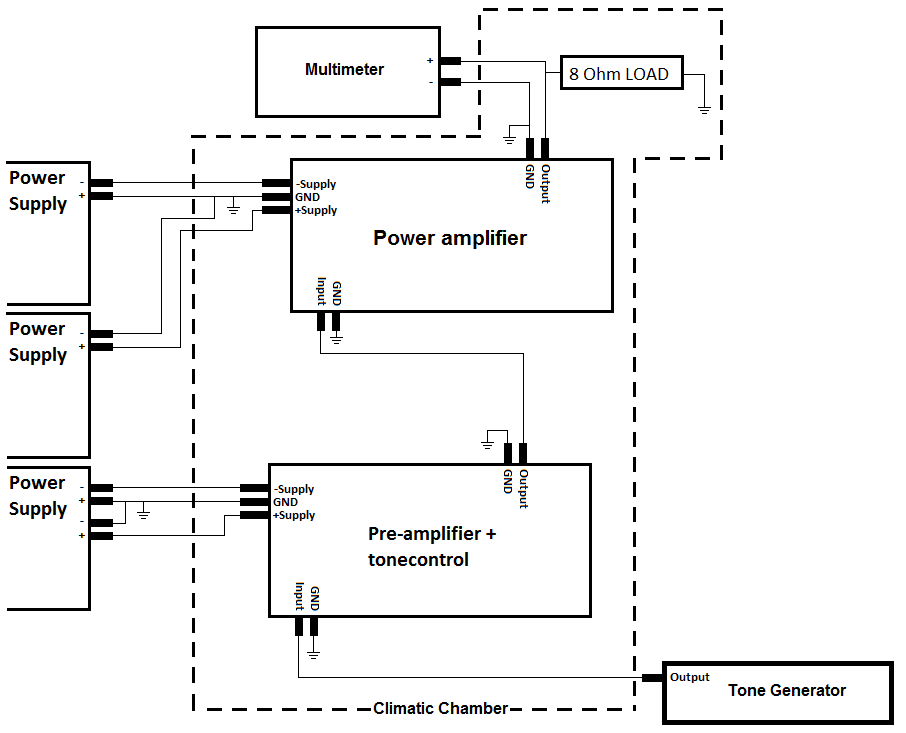
\includegraphics[width=.4\textwidth]{figures/filename}  %<--but is not needed.
  \caption{This image is clearly too small, remember to scale appropriately \fxnote{Remember source}}
  \label{fig:FigureLABEL}  %<--give the figure a label, so you can reference!
\end{figure}               %   For the label to work it must be under the caption.

% Fxnotes will not compile properly inside the figure, only in the caption.
% When \fxnote{} is used in caption, it does not show in a footnote as it normally 
% would, it does however appear in list of corrections.

\autoref{fig:FigureLABEL} $\leftarrow$ use autoref, unless you are referring to multiple pictures, then do like this: \autoref{fig:HbridgeClokwise4Q} and \ref{fig:HbridgeCounterClokwise4Q}.

%Do NOT use \vspace{length}, \hspace{length} or \noindent etc. unless exceedingly necessary - LaTeX is a markup language, let it do its job.
\vspace{.5cm}
\noindent
%
%--------- BIBLIOGRAPHY REF EKSAMPLE -----------------------------------
This reference only represents this line since it is before the punctuation mark\cite{YDing}. This next reference however represents the entire section. That is, all of the preceding sentences in the entire section. This is due to the fact that it is now after the punctuation mark in the end of the section (this is not used in the middle of a section!).\cite{YDing}

%>>PLEASE ALSO READ THE NOTE IN bibliography/bibliography.bib<<

Here is a way to make two images appear on the side of each other. Also, if you modified an image, this is how you properly refer to its original source:

\begin{figure}[H]
    \subcaptionbox  %<--use captionbox instead if no global caption is needed
    {               %                                \%-%-%-%-%-%-%\
      Clockwise 4Q operation.\newline                              %\
      \emph{Edited from image by Biezl.\cite{Biezl}}                %\
      \label{fig:HbridgeClokwise4Q}                                  %\
    }                                                                 %\
    {                                                                  %\
      \includegraphics[width=.46\textwidth]{HbridgeClockwise4Q}         %\
    }                                                                    %\
    \hspace{5pt}                                                          %\
    \subcaptionbox  %<-----------------------------------------------------%\
    {                                                                       %\
      Counterclockwise 4Q operation.\newline                                 %\
      \emph{Edited from image by Biezl.\cite{Biezl}}                          %\
      \label{fig:HbridgeCounterClokwise4Q}                                     %\
    }                                                                           %\
    {                                                                            %\
      \includegraphics[width=.46\textwidth]{HbridgeCounterClockwise4Q}            %|
    }                                                                             %|
    \caption{The 4 quadrant H-bridge configuration shown in both directions.}%<-%-/
    \label{fig:Hbridges}
\end{figure}

As seen \autoref{fig:HbridgeCounterClokwise4Q} can be referred to on its own, or you can use \autoref{fig:Hbridges} to refer to both \autoref{fig:HbridgeClokwise4Q} and \autoref{fig:HbridgeCounterClokwise4Q}.

If the figures are not directly related you might not want to use \textbf{(a)} and \textbf{(b)}, but instead give each figure their own label, here is an example:

\begin{figure}[H]
    \captionbox
    {
      Clockwise 4Q operation.\newline
      \emph{Edited from image by Biezl.\cite{Biezl}}
      \label{fig:HbridgeClokwise4Q2}
    }
    {
      \includegraphics[width=.46\textwidth]{HbridgeClockwise4Q}
    }
    \hspace{5pt}
    \captionbox
    {
      Counterclockwise 4Q operation.\newline
      \emph{Edited from image by Biezl.\cite{Biezl}}
      \label{fig:HbridgeCounterClokwise4Q2}
    }
    {
      \includegraphics[width=.46\textwidth]{HbridgeCounterClockwise4Q}
    }
\end{figure}

In this case \autoref{fig:HbridgeClokwise4Q2} can be referred to without involving \autoref{fig:HbridgeCounterClokwise4Q2}.

\pagebreak			 %|||||||
%			 \section{Table Sample} %to view this sample properly in the code, the screen must be
                       %wide enough, or you have to disable word-wrap in your editor.
\begin{table}[H]
\begin{tabular}{|l|p{5cm}|l|l|l|}
  \hline %-----------------------------------------------------------------------------------
  \textbf{No.} &\textbf{Description} &\textbf{Min} &\textbf{Max} &\textbf{Requirements}    \\
  \hline %-----------------------------------------------------------------------------------
  1            & Some Text           & Some Text   & Some Text   & Some Text               \\
               &                     &             &             & Some More Text          \\
               &                     &             &             & Text Text               \\
               &                     &             &             & Text Text Text          \\
  \hline %-----------------------------------------------------------------------------------
  2            & Some Text           & Some Text   & Some Text   & Some Text               \\
  \hline %-----------------------------------------------------------------------------------
  3            & By specifying the
                 width of a column
                 (|p\{5cm\}|) the
                 cells in that column
                 will not exceed the
                 specified width but         %Extra whitespace is used only for clarity
                 instead expand              %and will not affect the compiled output.
                 downward.
                                     & Some Text           & Some Text   & Some Text       \\
  \hline %-----------------------------------------------------------------------------------
  4            & Some Text           & Some Text   & Some Text   & Some Text               \\
  \hline %-----------------------------------------------------------------------------------
  \multicolumn{2}{|l|}{Some Text}    & \multicolumn{3}{l|}{Some Text}                      \\
  \hline %-----------------------------------------------------------------------------------
  \multicolumn{2}{|l|}{Text Text}    & \multicolumn{3}{l|}{Text = Text}                    \\
  \multicolumn{2}{|l|}{}             & \multicolumn{3}{l|}{Text = Text}                    \\
  \multicolumn{2}{|l|}{}             & \multicolumn{3}{l|}{Text = Text}                    \\
  \multicolumn{2}{|l|}{}             & \multicolumn{3}{l|}{Text = Text}                    \\
  \multicolumn{2}{|l|}{}             & \multicolumn{3}{l|}{Text = Text}                    \\
  \hline %-----------------------------------------------------------------------------------
  \multicolumn{2}{|l|}{Some Text}    & \multicolumn{3}{l|}{Teeeexxtt}                      \\
  \multicolumn{2}{|l|}{}             & \multicolumn{3}{l|}{\LaTeX}                         \\
  \hline %-----------------------------------------------------------------------------------
\end{tabular}
\caption{This Is a Table\label{table:TableLABEL}}
\end{table}

\autoref{table:TableLABEL} $\leftarrow$ use autoref, unless you are referring to multiple tables, then do like this: \autoref{table:TableLABEL} and \ref{table:TableLABEL}.

\pagebreak 		     %|||||||
%			 \section{Equation Sample} %<--In American English all Important Words in
                          %   Headlines are with Big Letters

% \unit is a macro. It uses SI units and aligns all the units neatly :)

\textbf{A normal equation:}
\begin{flalign}
  J_m \cdot \dot{\omega}_m(t) &= \tau_m(t) - B_m \cdot \omega_m(t) - r_m \cdot f_c(t)& \unit{N \cdot m}
  \label{eq:MotorGearNewtonSecLaw}
\end{flalign}
%
\begin{where}
  \va{ J_m               }{is the motor's inertia}                     {kg \cdot m^2}
  \va{ \omega_m(t)       }{is the angular velocity of the motor}       {rad \cdot s^{-1}}
  \va{ \dot{\omega}_m(t) }{is the angular acceleration of the motor}   {rad \cdot s^{-2}}
  \va{ \tau_m(t)         }{is the torque delivered by the motor}       {N \cdot m}
  \va{ B_m               }{is the motor's friction coefficient}        {N \cdot m \cdot s \cdot rad^{-1}}
  \va{ r_m               }{is the radius of the gear, $G_m$}           {m}
  \va{ f_c(t)            }{is the contact force between the two gears} {N}
\end{where}

\textbf{If you need to write something with numbers:} %<--Do not use \textbf{} as headlines, it is bad practice
                                                      %   use instead \chapter{}, \section{}, \subcaption{}, \subsubsection{}
                                                      %   in that order - never a \subsubsection{} directly under a \section{}
\begin{flalign}
  B      &= \num{2,2}\cdot 10^{-6}  \ \si{N\cdot m \cdot rad^{-1} \cdot s}& \label{eq:eq2} \\ %<-- if you want two equations to
  \tau_c &= \num{0.0016}            \ \si{N\cdot m}                       & \label{eq:eq3}    %    allign in one envirenment,
\end{flalign}                                                                              %    remember \\
%using \num{} ensures the same use of decimal point throughout the repport
%should you want to change it, the option is set in the preamble, just change 'period' to 'comma':
%\sisetup{decimalsymbol=period}

\autoref{eq:MotorGearNewtonSecLaw} $\leftarrow$ use autoref, unless you are referring to multiple equations, then do like this: \autoref{eq:eq2} and \ref{eq:eq3}.

\pagebreak		 %|||||||
%			 \section{TikZ Sample}

\textbf{TikZ is only for very patient people, I can recommend Inkscape with textext plugin: \url{https://pav.iki.fi/software/textext/}, difficult to install easy to use, and, if used carefully, nice results.}

%heavily commented example
\input{chapters/tikz/TikZblockDiagramSample.tex}

%way to keep the drawing code in a seperate file
\begin{figure}[H]
	\input{chapters/tikz/smallBlockDiagram.tikz}
	\centering
	\caption{Block diagram}
\end{figure}

%TikZ can also be used for circuits
\input{chapters/tikz/TikZcircuitSample.tex}


\pagebreak            %|||||||
%			 \section{Code Sample}

\begin{lstlisting}[ style=cstyle,
                    caption={C Code}, 
                    label=lst:cExample ]
#include "functions.h"

// Constant matrices
const float L[3] = { -11.0, -12.0, -13.0 };
const float B1[4] = { 0.0, -0.2396, 0.0, 0.2396 };
const float B2[4] = { 0.2396, 0.0, -0.2396, 0.0 };
const float B3[4] = { 0.0377, -0.0377, 0.0377, -0.0377 };
\end{lstlisting}

In \autoref{lst:cExample} is some C-code, and here is some in-line C-code: \inlinec{xTaskCreate();}.

\begin{lstlisting}[ style=pythonstyle,
                    caption={Python Code}, 
                    label=lst:pythonExample ]
# This parses the packets to identify messages and decodes them for the logs
class packetParser():
    def __init__(self,accelfile,gpsfile,measstate,fulllog,plog):
        self.GPS = {0: 'Latitude',
                    1: 'Longtitude',
                    2: 'Velocity'}
        self.IMU = {0: 'AccelerationX',
                    1: 'AccelerationY',
                    2: 'AccelerationZ',
                    3: 'GyroscopeX',
                    4: 'GyroscopeY',
                    5: 'GyroscopeZ',
                    6: 'MagnetometerX',
                    7: 'MagnetometerY',
                    8: 'MagnetometerZ',
                    9: 'Temperature'}
        self.MsgID = {0: self.GPS, 1: self.IMU}
        self.DevID = {0: 'GPS', 1: 'IMU'}
        self.accelburst = [0,0,0,0,0,0,0]
        self.accellog = accelfile
        self.fulllog = fulllog
\end{lstlisting}

In \autoref{lst:pythonExample} is some Python-code, and here is some in-line Python-code:\\ \inlinepython{self.plog.write(str(msgnr))}

\begin{lstlisting}[ style=matlabstyle,
                    caption={Matlab Code}, 
                    label=lst:matlabExample ]
  close all
  clear
  clc
  
  % Parameters
  mx=200;     % [kg] mass + added mass in xb direction
  my=250;     % [kg] mass + added mass in yb direction
  Iz=700;     % [kgm2]
  
  dx=70;      % [kg/s] 
  dy=100;     % [kg/s]
  dyaw=50;    % [kgm2/s]
\end{lstlisting}

In \autoref{lst:cExample}, \ref{lst:pythonExample} and \ref{lst:matlabExample} is some code, and here is some in-line matlab: \inlinematlab{randn(50)}            %|||||||
%|||||||                                                 ||||||||
%||||||||||||||||||||||||||||||||||||||||||||||||||||||||||||||||
%||||||||||||||||||||||||||||||||||||||||||||||||||||||||||||||||


%%% Prereport %%%
\setlength\cftaftertoctitleskip{2pt}
\setlength\cftafterloftitleskip{6pt}
\setlength\cftafterlottitleskip{6pt}
%\selectlanguage{danish}
%\title{Testing the performance of linear regressors using inertial information combined with sEMG to minimize the limb position effect in proportional and simultaneous control of lower arm prosthetics.}

%%% Frontmatter Settings %%%
\pagestyle{empty} %disable headers and footers
\pagenumbering{roman} %use roman page numbering in the frontmatter I II...
\fancyfoot[RE,LO]{17gr7404} %page number on all pages
\fancyfoot[LE,RO]{\thepage}
\fancyhead[LE,LO,RE,RO]{}

%%% Introductory Formalities %%%
%\includepdf[pages={1}]{formalities/frontpage.pdf}
\clearpage
\thispagestyle{empty}

\begin{figure}[H]
	\raggedleft
	
\includegraphics[width=0.2\textwidth]{figures/aaulogo-da.png}
\end{figure} 

\vspace{5 cm}

\begin{center}	
	\begin{Huge}
		\textbf{Simultaneous and proportional control of reaching and grasping}\\
		\vspace{5 mm}
		P$7$ Masterproject - Autumn $2017$\\
		\vspace{3 mm}
	\end{Huge}
	{\Large Gruppe $17$gr$7404$}
\end{center}
\vspace*{\fill}

\begin{center}
	\line(1,0){400}
\end{center}

			% <--- the frontpage
\pagestyle{fancy}
%{\small
\strut\vfill % push the content to the bottom of the page
\noindent Copyright \copyright{} Aalborg University 2015\par
\vspace{0.2cm}

\noindent This report is compiled in \LaTeX, originally developed by Leslie Lamport, based on Donald Knuth's \TeX. The main text is written in \emph{Latin Modern} pt 12, designed by Bogusław Jackowski and Janusz M. Nowacki. 
%The document is compiled via the website \url{www.overleaf.com}, an online collaborative based \LaTeX-editor with instant preview, which enables multiple persons to edit the document simultaneously.
Flowcharts and diagrams are made using Microsoft Visio. 
\clearpage
%\begin{document} 
\thispagestyle{empty}
\begin{titlepage}
\begin{nopagebreak}
{\samepage 

\begin{tabular}{r}
\parbox{\textwidth}{  \raisebox{-15mm}{
\includegraphics[height=3cm]{figures/aaulogo-en.png}}
\hfill \hspace{2cm} \parbox{8cm}{\begin{tabular}{l} %4.90
{\small \textbf{\textcolor{aaublue}{{7\textsuperscript{th} Semester, Master Project}}}}\\
{\small \textbf{\textcolor{aaublue}{School of Medicine and Health}}}\\
%{\small \textbf{\textcolor{aaublue}{Communication Technologies}}}\\ 
{\small \textbf{\textcolor{aaublue}{Biomedical Engineering and Informatics}}}\\
{\small \textcolor{aaublue}{Fredrik Bajers Vej 7A}} \\
{\small \textcolor{aaublue}{9220 Aalborg}} \\
%{\small \textcolor{aaublue}{\emph{http://www.sict.aau.dk/electronics-and-it}}}
\end{tabular}}}
\end{tabular}

\begin{tabular}{cc}
\parbox{7cm}{

\textbf{Titel:}

title:\\ 

\textbf{Theme:}

\small{
Biomedical signals and information\\
}


\parbox{8cm}{


\textbf{Project period:}\\
P7, Autumn 2017\\
01/08/2017 - 19/12/2017\\
   
\textbf{Project group:}\\
17gr7404\\ %\fxnote{Input group number}
  
\textbf{Collaborators:}\\
Irene Uriarte \\
Martin Alexander Garenfeld \\
Oliver Thomsen Damsgaard \\
Simon Bruun \\

\textbf{Supervisors:}\\
Strahinja Dosen \\
Jakob Lund Dideriksen \\
Lotte N.S. Andreasen Struijk \\
}\\


\textbf{Pages:} 0\\
\textbf{Appendixes:} b \\
%\textbf{Ekstra:} For projektkode: Se forord\\ %eks. en CD eller USB
\textbf{Afsluttet:} 19/12/2017\\

\vfill } &
\parbox{7cm}{
  \vspace{.15cm}
  \hfill
  \begin{tabular}{l}
  {\textbf{Abstract}}\bigskip \\
  \fbox{
    \parbox{6.5cm}{\bigskip
     {\vfill{\small \lipsum[15]
%write real thing
     \bigskip}}
     }}
   \end{tabular}}
\end{tabular}} %\vspace{1cm}


\centering
\textit{Publication of this report's contents, including source references, may only happen in agreement with the authors.}\\
%\textit{Offentliggørelse af rapportens indhold, med kildeangivelse, må kun ske efter aftale med forfatterne.}\\


\end{nopagebreak}
\end{titlepage}
%\end{document} 			 % <--- the titlesheet - contains the synopsis!!
%%% Preface %%%
\cleardoublepage
%abstract
\section{Abstract}

\textbf{Background:} Electromyography (EMG) is widely used as input to control scheme of myoelectric prosthetics. However, EMG signals change with limb position and thus lowers the accuracy in classification.% and very few studies has assessed this problem. 
Inclusion of the use of Inertial Measurement Units (IMU) has proved to raise the accuracy in pattern recognition methods. However, pattern recognition methods provides only control of one degree of freedom (DoF) at a time, and are computational costly. This study propose to use the combination of EMG recordings and accelerometer data in a linear regression model to overcome the slower reaction time of pattern recognition systems and to enable a simultaneous and proportional control scheme. 


\textbf{Methods:} In this study recordings from four able-bodied subjects has been collected, performing four hand movements at the wrist in three different limb positions. The data is evaluated through principal component analysis (PCA) and processed/trained with a linear model to classify the hand movements. Eight regressors are trained for each test subject; four with and without using IMU data. The regressors are tested in a real-time visual environment on PC measuring time to complete a target-reaching task of eight targets. The performance of the regressors are compared between using the IMU data and not using IMU data to determine the effect of including IMU data. 


modified Fitts' Law 


\textbf{Results:} bad


\textbf{Conclusion:} no


\textbf{Keywords:?} surface electromyography, inertial measurement unit, simultaneous and proportional myoelectric control, regression, hand motion classification, hand prosthetic
			 % <--- this is the abstract!!
%\clearpage
\chapter*{Preface}

\lipsum[9]

\pagebreak				% <--- the preface

\pdfbookmark[0]{Table of Contents}{label: tableOfCentents}
\tableofcontents
\cleardoublepage


%%% Mainmatter Settings %%%
\pagenumbering{arabic} %use arabic page numbering in the mainmatter
\fancyfoot[RO,LE]{\thepage \text{ of} \pageref{LastPage}}
\fancyfoot[RE,LO]{17gr7404}
\fancyhead[RE,LO]{}
\fancyhead[RE,LO]{\color{aaublue}\small\nouppercase\leftmark} %even page - chapter title
\pagestyle{fancy}


%---------------------------INPUTS-------------------------------

%%%%%%%%%%%%%%%%%%%%%%%%%%%%%%%%%%%%%%%%%%%%%%%%%%%%%%%%%%%%%%%%%%%%%%%%%%%%%%%%%
%2345678901234567890123456789012345678901234567890123456789012345678901234567890
%        1         2         3         4         5         6         7         8

%\documentclass[letterpaper, 10 pt, conference]{ieeeconf}  % Comment this line out
% if you need a4paper
%\documentclass[a4paper, 10pt, conference]{ieeeconf}      % Use this line for a4
% paper



% The following packages can be found on http:\\www.ctan.org
%\usepackage{graphics} % for pdf, bitmapped graphics files
%\usepackage{epsfig} % for postscript graphics files
%%\usepackage{mathptmx} % assumes new font selection scheme installed
%%\usepackage{times} % assumes new font selection scheme installed
%%\usepackage{amsmath} % assumes amsmath package installed
%%\usepackage{amssymb}  % assumes amsmath package installed
%\usepackage{subfigure}
%\usepackage{float}
%
%\restylefloat{figure}

\title{\LARGE \bf
	The effect of limb position on myoelectric prosthetic control using linear regression
}%final name

%\author{ \parbox{3 in}{\centering Huibert Kwakernaak*
%         \thanks{*Use the $\backslash$thanks command to put information here}\\
%         Faculty of Electrical Engineering, Mathematics and Computer Science\\
%         University of Twente\\
%         7500 AE Enschede, The Netherlands\\
%         {\tt\small h.kwakernaak@autsubmit.com}}
%         \hspace*{ 0.5 in}
%         \parbox{3 in}{ \centering Pradeep Misra**
%         \thanks{**The footnote marks may be inserted manually}\\
%        Department of Electrical Engineering \\
%         Wright State University\\
%         Dayton, OH 45435, USA\\
%         {\tt\small pmisra@cs.wright.edu}}
%}

\author{Simon Bruun, Oliver Thomsen Damsgaard, Martin Alexander Garenfeld, Irene Uriarte}% <-this % stops a space

%\begin{document}

\setcounter{topnumber}{6}
\setcounter{bottomnumber}{6}
\setcounter{totalnumber}{10}
\renewcommand{\topfraction}{1}
\renewcommand{\bottomfraction}{1}
\renewcommand{\textfraction}{0}
\renewcommand{\floatpagefraction}{1}
		
	\maketitle
	\thispagestyle{empty}
	\pagestyle{empty}
	
	\begin{multicols}{2}

	%%%%%%%%%%%%%%%%%%%%%%%%%%%%%%%%%%%%%%%%%%%%%%%%%%%%%%%%%%%%%%%%%%%%%%%%%%%%%%%%
	\begin{abstract}
%		Electromyography (EMG) is widely used for controlling functional prosthetics. However, EMG signals for the same movements change with variations in limb position and lowers the accuracy in control schemes \cite{fougner2012}. Most of the previous studies have utilized classification for pattern recognition when changing limb position, with a negative effect in performance. %Linear regression is a newer method in control of myoelectric prosthetics, which has proven to yield robust simultaneous and proportional control \cite{hanhe2014}. %Only the RMS feature was previously tested in variations of limb positions in regression-based control \cite{hwang2017}. 
This study investigated the effect of limb position in a linear regression-based control scheme, when using 
%the commonly used 
Mean Absolute Value (MAV) and Logarithmic Variance (LogVar) as features. %where the latter has shown linear properties \cite{hanhe2014}.
Seven (more now) able-bodied subjects were recruited for data acquisition, performing four wrist movements in three different limb positions. One regression model was build to recognize the different wrist movements under study, taking into account both features. %One regression model %(regressor) 
%was build for each wrist movement for each test subject: four for each feature. 
The regressors were tested online in a virtual environment. %where the time to complete a target-reaching task of sixteen targets was measured. %The performance (time per reached target) of the online test was compared between the different limb positions of the same feature and between all limb positions of the two features through statistical analysis. 
%Using a Friedman's test the performance scores between the three limb positions prove not to be significantly different 
%(p = 0.5647), 
%when applying the LogVar trained regressors %in the online test. For the MAV trained regressors the performance score between all limb positions cannot be proven significantly different either (p = 0.1561). 
%There was no difference in the time to reach the targets across the two features %(LogVar: 6.5 s, MAV: 5.5 s; p = 0.13).
The results showed that changes in limb position do not affect the control when linear regression model is trained with the %MAV or LogVar 
features extracted. This is opposed to previous studies using classification as control scheme. Linear regression has the potential to be used in future control schemes for myoelectric prosthetics for use in daily life tasks.\\


\textit{\textbf{Keywords---}}surface electromyography, inertial measurement unit, simultaneous and proportional myoelectric control, regression, hand motion classification, hand prosthetic


Electromyography (EMG) is widely used for controlling functional prosthetics. However, EMG signals for the same movements change with variations in limb position and lowers the accuracy in control schemes \cite{fougner2012}. Most previous studies testing the effect of limb position, have utilized classification for pattern recognition with a negative effect in performance. This study investigated the effect of limb position in a linear regression-based control scheme, when using Mean Absolute Value and Logarithmic Variance as features, and including IMU data to improve the performance of the regression models. 12 able-bodied subjects were recruited for data acquisition, performing four wrist movements in three different limb positions. One regression model was build to recognize the different wrist movements under study, taking into account both features. The regressors were tested online in a virtual environment. The results showed that changes in limb position do not affect the control when linear regression model.
This is opposed to previous studies using classification as control scheme. Linear regression has the potential to be used in future control schemes for myoelectric prosthetics for use in daily life tasks.\\
		
\textit{\textbf{Keywords---}}surface electromyography, inertial measurement units, simultaneous and proportional myoelectric control, linear regression, lower arm prosthetics.
	\end{abstract}
	
	%%%%%%%%%%%%%%%%%%%%%%%%%%%%%%%%%%%%%%%%%%%%%%%%%%%%%%%%%%%%%%%%%%%%%%%%%%%%%%%%
	
\section{INTRODUCTION}%%%%%%%%%%%%%%%%%%%%%%%%%%%%%%%%%%%%%%%%%%%%%%%%%%%%%%%%%%%%%%
		
%		%What has been done in the EMG-prosthesis area?
In recent years the development of EMG controlled lower arm prosthetics has advanced considerably, due to an increased interest in the area along with higher demands for better prosthetics and more precise control. \cite{Fougner2012} In the early years most EMG prosthetics functioned by controlling one degree of freedom (DOF) with on-off control, mainly by linking antagonistic muscles to one DOF. This kind of prostheses change between states due to a switching impulse which cause a state machine to shift its present state. Usually a strong and fast muscle contraction from the users is employed to generate the switching signals. \cite{amsuess2014}
This type of control provided users a way to control more than one DOF, but never simultaneously. The switch-control functioned on a cycle, so users would have to go through all the movements of the prosthesis to find the one they wanted to perform. However, as demands rose, more complex methods was introduced to the EMG prosthetics scene. Classification methods effectively enabled users to use DOF's more freely because the switching was now replaced by direct recognition of different muscle contractions linked to specific prosthetic movements. This also effectively enabled proportional control of movements, but gave rise to new problems: a wider range of control would give less accurate movements, and training the classifiers proved difficult, as the training could over-fit, causing extended use of the prosthetics to degrade in performance. \cite{Ison2016}

%Regression
Introducing regression as a new mapping method in myoelectric prosthetics provided a way to enable both simultaneous and proportional control of multiple DOF's. Regression is able to provide a continuous value for each DOF based on the recorded EMG signal, while a classifier only decides upon a certain class. \cite{hahne2014, jiang2010}
This means that classification can only translate a recorded EMG signal to one movement of the prosthetic at a time. It can do so proportionally but the handling still lacks natural control, since movements by able-bodied individuals very rarely only happen in one DOF at a time. Regression methods constantly provide a value, and since several regressors can be used at a time, several values can be used in the recognition of movements. This is what enables regression methods to perform simultaneous and proportionally. 

Applying regression as a mapping method in proportional and simultaneous control of multiple DOF's has been shown to perform well in recognition of movements and doing so with a low computation time. \cite{hahne2014} However, very few studies have tested the regressor performance in daily life tasks outside the clinical training environment. \cite{jiang2012} A study by Fougner et al. \cite{Fougner2011} has addressed the problem that most studies test their method on only one limb position. This means that the actual performance of regression methods has not yet been properly addressed when recognizing movements, where the arm changes position during daily life tasks. 

%Which issues are there in the EMG-prosthesis area?(decreasing quality of control of hand gestures when the arm is placed in different positions)
When recording EMG signals it has been shown that some muscles are activated based on joint angles, even though the muscles are not involved in the movement of that joint \cite{Fougner2011}. This provides a problem, but can be explained by muscle-synergies \cite{DeRugy2013}. These muscle-synergies are created by the Central Nervous System (CNS) and coordinated into activation of different muscles at varying times. This enables the CNS to control the muscle-synergies instead of controlling each muscle individually to perform movements \cite{jiang2009}. This means that muscles in the lower arm can be activated when muscles in the upper arm are activated, in a level that will be detectable in EMG recordings, and enough to alter recognition of movements, when the arm is active in limb positions other than those tested in a clinical environment. 

%What would be novel to add to this area?(adding IMU’s to a regressor, since it has been done with a classifier)
In order to overcome the problem of muscles-synergies, Fougner et al. \cite{Fougner2011} has suggested to combine recordings of EMG signals with inertial information to provide limb position data. This could be beneficial in increasing the accuracy of EMG controlled prosthetics for use in daily life tasks. 
Even though the combination of EMG and Inertial Measurement Unit (IMU) data has been proposed as a valid way to improve the performance and accuracy of EMG based prosthetics, it has only been investigated in few studies. \cite{Roy2010, Imtiaz2014, jiang2012}

To the authors knowledge the combination of EMG recordings and IMU data has only been done with classification methods. A novel approach to further investigate the usability of combining EMG and IMU is to build a regression based control scheme for myoelectric prosthetics. This would enable both proportional and simultaneous control of several DOF's, where the inclusion of IMU data should provide more information on limb position to counter the effect of limb position.






%In recent years the development of EMG controlled prosthesis have advanced due to an increased interest in the area as well as a higher demand of better control of this prosthesis.\cite{fougner2012}
%In the early years most EMG prosthetics functioned by only controlling one DOF by \textit{on-off control}, mostly by linking antagonistic muscles to one DOF. %This along with \textit{mode switching} provided users a way to control more than one DOF, but not in a simultaneous way. 
%This control provided a way to control more than one DOF, but not simultaneously. However, as demands would rise, more complex methods were introduced to the EMG scene. Classification methods enabled simultaneous control of more than one DOF, but gave rise to new problems; a wider range of control would give less accurate movements, and training the pattern recognition methods proved difficult, as the training could over-fit, causing extended use of the prosthetics to degrade in performance. \cite{Ison2016}.
% 
%It has been proved that regression techniques can be apply as a new mapping method to achieve simultaneous and proportional control of multiple DOFs\cite{hanhe2014}. Regression methods provide a continous value for each DOF based on the recorded EMG signal, while classification methods only decides upon a certain class. However there are still difficulties when prosthesis perform outside the clinical training environment\cite{jiang2012}.
% Fougner et al.\cite{Fougner2011} noticed that majority of studies only take in account one limb position. It has been shown that some muscles are activated based on joint angles \cite{reference}, even though the muscles are not involved in the movement of that joint, which can be explained by muscle-synergies existed between muscles.
%% which becomes a problem since muscles create muscle-synergies to perform movements. 
%Variations in limb positions can have an impact on the robustness of EMG pattern recognition. %To be able to offer a good perform of the prosthesis, these should be able to execute with the same accuracy diverse hand gestures in different limb positions. 
%In order to overcome this problem it has been suggested to combine EMG data as well as IMU data, to provide limb position information. Nevertheless this combination of data have only been investigated for classification methods. 
%In this study we test the performance of linear regression methods combining EMG and IMU data for a simultaneous and proportional control of two DOFs in a lower-arm prothesis while the arm is located in different limb positions.
%% in the training sesions of the regressor to obtain simultaneous and proportional control of EMG prosthesis. 
%%Hypotheses
%%Simultaneous and proportional control of two  DOF's of the wrist in different limb positions, can be achieve trough the use of linear regression as control system. Combining EMG and IMU's can minimize the limb position effect when using regression as control system.
In recent years the development of EMG controlled lower arm prosthetics has advanced considerably, due to an increased interest in the area along with higher demands for better prosthetics and more precise control. \cite{Fougner2012} In the early years most EMG prosthetics functioned by controlling one degree of freedom (DOF) with on-off control, mainly by linking antagonistic muscles to one DOF. This kind of prostheses change between states due to a switching impulse which cause a state machine to shift its present state. Usually a strong and fast muscle contraction from the users is employed to generate the switching signals. \cite{amsuess2014}
This type of control provided users a way to control more than one DOF, but never simultaneously. The switch-control functioned on a cycle, so users would have to go through all the movements of the prosthesis to find the one they wanted to perform. However, as demands rose, more complex methods was introduced to the EMG prosthetics scene. Classification methods effectively enabled users to use DOF's more freely because the switching was now replaced by direct recognition of different muscle contractions linked to specific prosthetic movements. This also effectively enabled proportional control of movements, but gave rise to new problems: a wider range of control would give less accurate movements, and training the classifiers proved difficult, as the training could over-fit, causing extended use of the prosthetics to degrade in performance. \cite{Ison2016}

Introducing regression as a new mapping method in myoelectric prosthetics provided a way to enable both simultaneous and proportional control of multiple DOF's. Regression is able to provide a continuous value for each DOF based on the recorded EMG signal, while a classifier only decides upon a certain class. \cite{hahne2014, jiang2010}
This means that classification can only translate a recorded EMG signal to one movement of the prosthetic at a time. It can do so proportionally but the handling still lacks natural control, since movements by able-bodied individuals very rarely only happen in one DOF at a time. Regression methods constantly provide a value, and since several regressors can be used at a time, several values can be used in the recognition of movements. This is what enables regression methods to perform simultaneous and proportionally. 

Applying regression as a mapping method in proportional and simultaneous control of multiple DOF's has been shown to perform well in recognition of movements and doing so with a low computation time. \cite{hahne2014} However, very few studies have tested the regressor performance in daily life tasks outside the clinical training environment. \cite{jiang2012} A study by Fougner et al. \cite{Fougner2011} has addressed the problem that most studies test their method on only one limb position. This means that the actual performance of regression methods has not yet been properly addressed when recognizing movements, where the arm changes position during daily life tasks. 

When recording EMG signals it has been shown that some muscles are activated based on joint angles, even though the muscles are not involved in the movement of that joint \cite{Fougner2011}. This provides a problem, but can be explained by muscle-synergies \cite{DeRugy2013}. These muscle-synergies are created by the Central Nervous System (CNS) and coordinated into activation of different muscles at varying times. This enables the CNS to control the muscle-synergies instead of controlling each muscle individually to perform movements \cite{jiang2009}. This means that muscles in the lower arm can be activated when muscles in the upper arm are activated, in a level that will be detectable in EMG recordings, and enough to alter recognition of movements, when the arm is active in limb positions other than those tested in a clinical environment. 

In order to overcome the problem of muscles-synergies, Fougner et al. \cite{Fougner2011} has suggested to combine recordings of EMG signals with inertial information to provide limb position data. This could be beneficial in increasing the accuracy of EMG controlled prosthetics for use in daily life tasks. 
Even though the combination of EMG and Inertial Measurement Unit (IMU) data has been proposed as a valid way to improve the performance and accuracy of EMG based prosthetics, it has only been investigated in few studies. \cite{Roy2010, Imtiaz2014, jiang2012}

To the authors knowledge the combination of EMG recordings and IMU data has only been done with classification methods. A novel approach to further investigate the usability of combining EMG and IMU is to build a regression based control scheme for myoelectric prosthetics. This would enable both proportional and simultaneous control of several DOF's, where the inclusion of IMU data should provide more information on limb position to counter the effect of limb position.		
	
\section{METHODS}%%%%%%%%%%%%%%%%%%%%%%%%%%%%%%%%%%%%%%%%%%%%%%%%%%%%%%%%%%%%%%%%%%%
	
%		\subsection{Experimental Setup}
EMG data was collected from (define number) able-bodied subjects. The subjects performed four different hand gestures. This study is only focus on two DOF, which are, flexion, extension, radial and ulnar deviation of the wrist. The order in the execution of the movements was the same for each subject. EMG signals were recorded with Myo armband, positioned in the right forearm of the subjects (all subjects right handed). The procedure was performed in three different limb positions. In order to avoid shoulder fatigue a relaxation period was given between trials. The subjects were instructed not to move the fingers during the data acquisition. The process was performed in a standing position. \\ %figure hand and limb positions
 Myo armband counts with eight medical grade stainless steel surface EMG sensors. %It is capable of pulling EMG data at a sample rate of 200 Hz. 
 Furthermore its nine axis IMU provides information about position and orientation of the arm combining three axis accelerometer, three axis gyroscope and three axis magnetometer.\\   
 In order to acquire the training data necessary to build the regressor, a graphical user interface (GUI) was implemented in MATLAB. %Firstly baseline was meassure holding the forearm relaxed and the wrist in a neutral position for the corresponding limb position. This measure was substracted from the signal afterwards to be able to remove the present artefacts. Subsequently maximum voluntary contraction (MVC) was meassure. The MVC  was calculated as a mean of the maximum values in each of the eight cannels, and was set as a normalized reference point of 1.
 %The data acquisition was depicted through a trapeze. MVC was set as the desired value before data acquisition. Consequently each hand gesture was performed as a fraction of the MVC. At the begining of the training data collection two second resting phase was given followed by two seconds ascending slope to reach the plateau phase, with a duration of three seconds. Afterwards a descending phase of two seconds and a resting phase of one second finalized the data acquisition. The total acquisition time was ten seconds per hand movement.

	%\subsection{Maintaining the Integrity of the Specifications}
	
	%The template is used to format your paper and style the text. All margins, column widths, line spaces, and text fonts are prescribed; please do not alter them. You may note peculiarities. For example, the head margin in this template measures proportionately more than is customary. This measurement and others are deliberate, using specifications that anticipate your paper as one part of the entire proceedings, and not as an independent document. Please do not revise any of the current designations
	
	\subsection{Preprocessing}
	For this study the EMG data acquired were filtered using a second-order Butterworth high-pass filter, cutoff frequency ($f_c$=10Hz), to avoid low frequency movement artefacts in the recorded signal.\\
	%review two states part trapeze!!
	%The EMG signal is the result of the addition of different motor unit action potential trains (MUAPTs). Through the data acquisition phase EMG signal can be divided into two main states. The transient state, related with the beginning phase of the muscle contraction and the steady state which is the stable phase of the muscle contraction when a constant position is held \cite{mobarak2014}. Although the steady state only contains a short temporal structure of the patterns involved in the contraction of the muscle \cite{mobarakm2014}, studies has shown that it is possible to achieve online continuous control using steady state EMG signals.This could be due to the fact that a larger amount of meaningful data is contained in this muscle contraction phase \cite{mobarakm2014}. For the training of the control system in this project the steady signal was then used.
	
	\subsection{Feature extraction}
	The features were extracted creating a sliding-window of 40 samples. % with an overlapping of the 50\%. 
	Two different time domain features were extracted, MAV as well as LogVar. MAV represent the amplitud of the signal. It is defined as the average of the absolute values of the EMG signal and expresed as:
	\begin{equation}
	MAV = \frac{1}{N}\sum\limits_{i=1}^N|x_i|
	\end{equation}
	where N is the length of the signal, and $x_i$ is the signal of $i$ samples.
	The LogVar is a nonlinear transformation of the variance, which has been shown to behaves more linear than other time domain features. \cite{hanhe2014}
	\begin{equation} \label{eq:logvar}
	log(\sigma^2) = log(\frac{\sum\limits_{i=1}^N(x_i - \mu)^2}{N})
	\end{equation}
	where N expresses the length of the signal, $x_i$ is the $i^th$ sample of the signal and $\mu$ is the mean.
	\subsection{Separability of data}
Principal Component Analysis (PCA) was applied to be able to evaluate the quality of the features extracted from the EMG signals.
	%This analysis tool express a set of correlated variables into non-correlated components. In that way, the data set can be expressed in a reduced dimensionality hyperspace using less but most representative variables which are the principal components. Through PCA is  possible to see significant outliers or if the clusters formed by the features can be easily distinguishable. This was done to avoid inaccurate training of the regressors. PCA was performed for each movement in each limb position. %and represented in three dimensional space.figure? 
	\subsection{Data exclusion}
	Some of the subjects were not able to perform through the study properly. In order to ensure constant data those subjects were exclude.
	\subsection{Regression models}
	The acquired data was used to built the different regressors that had been implemented, one for each movement under study and for both features. Multivariate linear regression as an extension of simple linear regression had been applied as is shown in \ref{reg}:
\begin{equation}
	\hat{Y} = \alpha + \beta_1 X_{1} + \beta_2 X_{2} + ... + \beta_i X_{i} + \epsilon_i
		\label{reg}
\end{equation}
	where $Y$ is the dependent variable, $X_i$ are the independent variables, $\beta_i$ is the regression coefficient in the sampled population, $\alpha$ is the predicted value of $Y$ at $X = 0$ and $\epsilon$ is the error.
	
	\subsection{Regressor accuracy}
	Superimposition\\
	In order to examine the performance of the regressors the estimations of the regressor and the actual data for the two different features extracted had been superimposed. Thereby the behave of the regressor can be shown at different intensities and movements. Consequently whether other regression methods should be considered to obtain a lower error.\\
	RMSE\\
	To meassure the accuracy of the regressor, Root Mean Squared Error (RMSE) was calculated. RMSE is a calculation of the standard deviation of the residuals, that is, the difference between the estimated and the actual values.
	%equation
	\begin{equation}
	RMSE = \sqrt{\frac{\sum\limits_{i=1}^N(y_i - \hat{y_i})^2}{N}}
	\end{equation}
	Where N is the length of the signal, $y_i$ is the $i^th$ variable of the actual data and $\hat{y_i}$ is the $i^th$ output of the regressor. The RMSE will be done for the regressor of each movement.\\
	
	%Fitts Law\\
	%A modified version of Fitts' Law had been used to quantify the performance of the trained regressors. Fitts' Law describes that, the time it takes to do a rapid movement to reach a target area, is dependent on the distance to the target area, and the size of the target area. The law demonstrates that the information of any human motor tasks, is finite and only limited by the capabilities of the control system. The control exhibit a negative correlation between speed and accuracy. \cite{Kamavuako2014}
	%Fitts' Law calculates an \textit{Index of Difficulty} (ID) by \ref{eq:Fitts}
	
%	\begin{equation} \label{eq:Fitts}
	%ID = log_{2} \cdot (\frac{2D}{W})
	%\end{equation}
	
	%where D is distance to the targets and W is width of target area. The system in this study does not provide a reasonable scale for distance and target width, for this reason Fitts' Law cannot be apply as usual. Instead, the time it takes a subject to reach the targets as well as the number of targets reached will be noted to calculate a performance score as shown in \ref{eq:ourScore}.
	
	%\begin{equation} \label{eq:ourScore}
	%Score = \frac{time}{targets\ reached}
	%\end{equation}
	%Consequently low score results represent the best performance.
	%To accomplish the modified Fitts' Law test a compass-plot was implemented in the GUI Fig.\ref{figurelabel}. The subjects had to reach 16 targets distributed around the origin in two different radius. This allows to test the proportional control. The targets were fixed in the diagonals of the compass-plot to be able to test simultaneous control. The amount of targets reached in each quadrant gives important information about the regressor performance as well as, providing the weak directions.
	
	
	

\subsection{Subjects}
For the experiment 12 able-bodied subjects were recruited (10 male, 2 female - 11 right-handed, 1 left-handed) by contacting fellow undergraduate biomedical engineering students at Aalborg University. All subjects participated in the entire experiment, and were initially informed of the research aim, and instructed about the procedures during the experiment. Entire data sets from three subjects were excluded. The cause for exclusion for one subject was due to data that did not correspond with the instructed movements, and the remaining two was due to baseline data being similar in amplitude compared to EMG amplitude of high contraction movements. All subjects participated voluntarily, and did not receive any monetary reimbursement. 

\subsection{Data acquisition}
EMG signals and inertial information were recorded with the Myo armband from Thalmic Labs - an 8 channel dry electrode armband with 200 Hz EMG sampling rate and 50 Hz IMU sampling rate. Only accelerometer data from the IMU was acquired for data processing. The Myo armband has been suggested as a suitable data acquisition system for pattern classification \cite{Mendez2017}, but not yet for a regression-based control scheme. 
The armband was placed around the thickest part of the dominant forearm, approximately 1/4 of the length towards the wrist distal of the elbow. For a close contact between the forearm and armband, clips were used to tighten the fit if necessary. All data acquisition, processing, data analysis and testing was performed in MATLAB and MATLAB's Graphical User Interface Development Environment.

In the training data acquisition the subjects were instructed to perform four different wrist movements of 2 DOF's depicted in figure \ref{fig:wristmovement} in three different limb positions depicted in figure \ref{fig:limbpositions}. Each movement was performed with four different EMG intensities of the Maximum Voluntary Contraction (MVC) in each limb position (baseline, 30\%, 50\% and 80\%). To ensure that correct fractions of the EMG intensity were recorded, a Graphical User Interface (GUI) was build to provide real-time feedback for the subject. Initially the MVC was recorded and set as reference point for the following trials. A trapeze was drawn for each data acquisition trial, where the plateau depicted the desired fraction of the MVC. A cursor visualized the EMG signal, and moved horizontally and continuously with time. The vertical position of the cursor was calculated as the mean of the absolute EMG signal across all channels in a 200 ms window, and scaled between 0 and 1 according to the MVC. The subject adjusted the height of the cursor by varying the contraction intensity, and was instructed to follow the trapeze as precise as possible. Only the plateau of the trapeze was used in data processing. A study have shown that it is possible to achieve online continuous control using steady-state EMG signals \cite{mobarak2014}. The duration of each data acquisition trial was 10 s, where the plateau phase was 3 s. To avoid fatigue the subjects had a 10 s break between trials of different intensities. Between limb position trials subjects were given a 5 min rest. Accelerometer data was additionally recorded in each trial. All trials were performed while standing.
Additional 50\% of MVC EMG data was acquired for each wrist movement in all limb positions for offline testing.

The recorded EMG data was filtered using a $2^{nd}$ order Butterworth high-pass filter with a 10 Hz cut-off to remove movement artefacts. 

\begin{figure}[H]
	\centering
	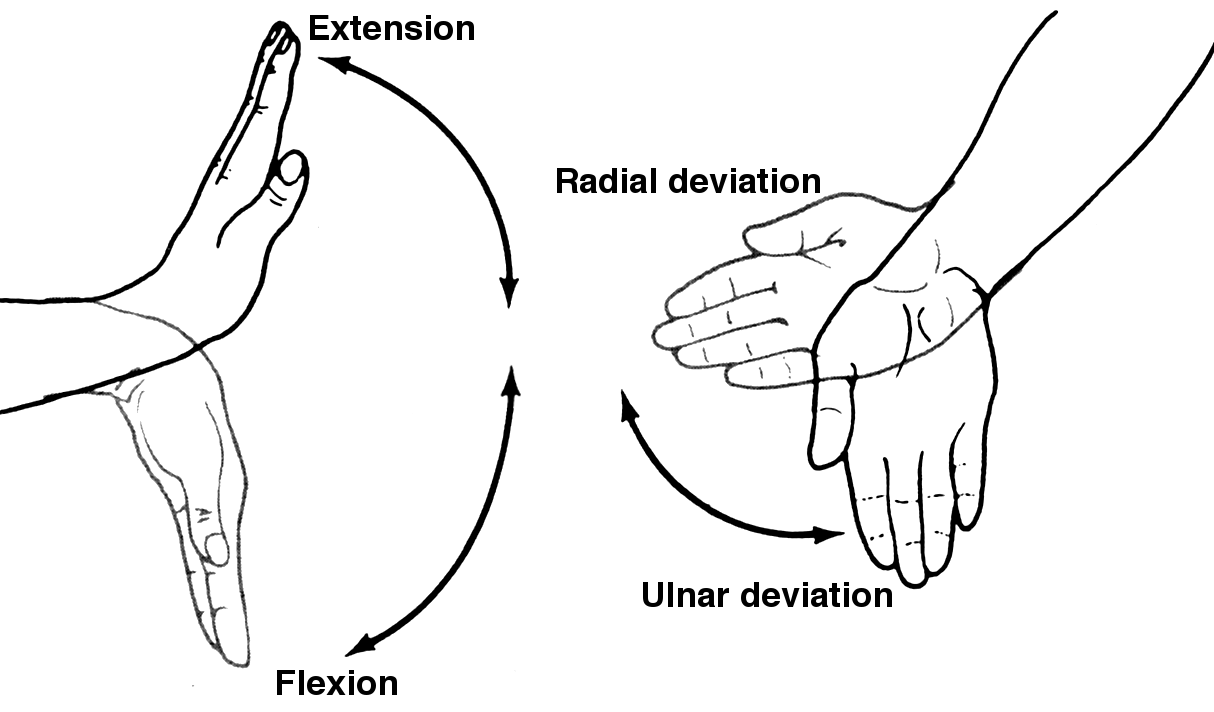
\includegraphics[width=0.4\textwidth]{figures/paperFigures/wristmovement}  %<--but is not needed.
	\caption{Illustration of the two DOF's used in the study (P1: flexion, P2: extension and P3: radial deviation, P4: ulnar deviation)}
	\label{fig:wristmovement}  %<--give the figure a label, so you can reference!
\end{figure}

\begin{figure}[H]
	\centering
	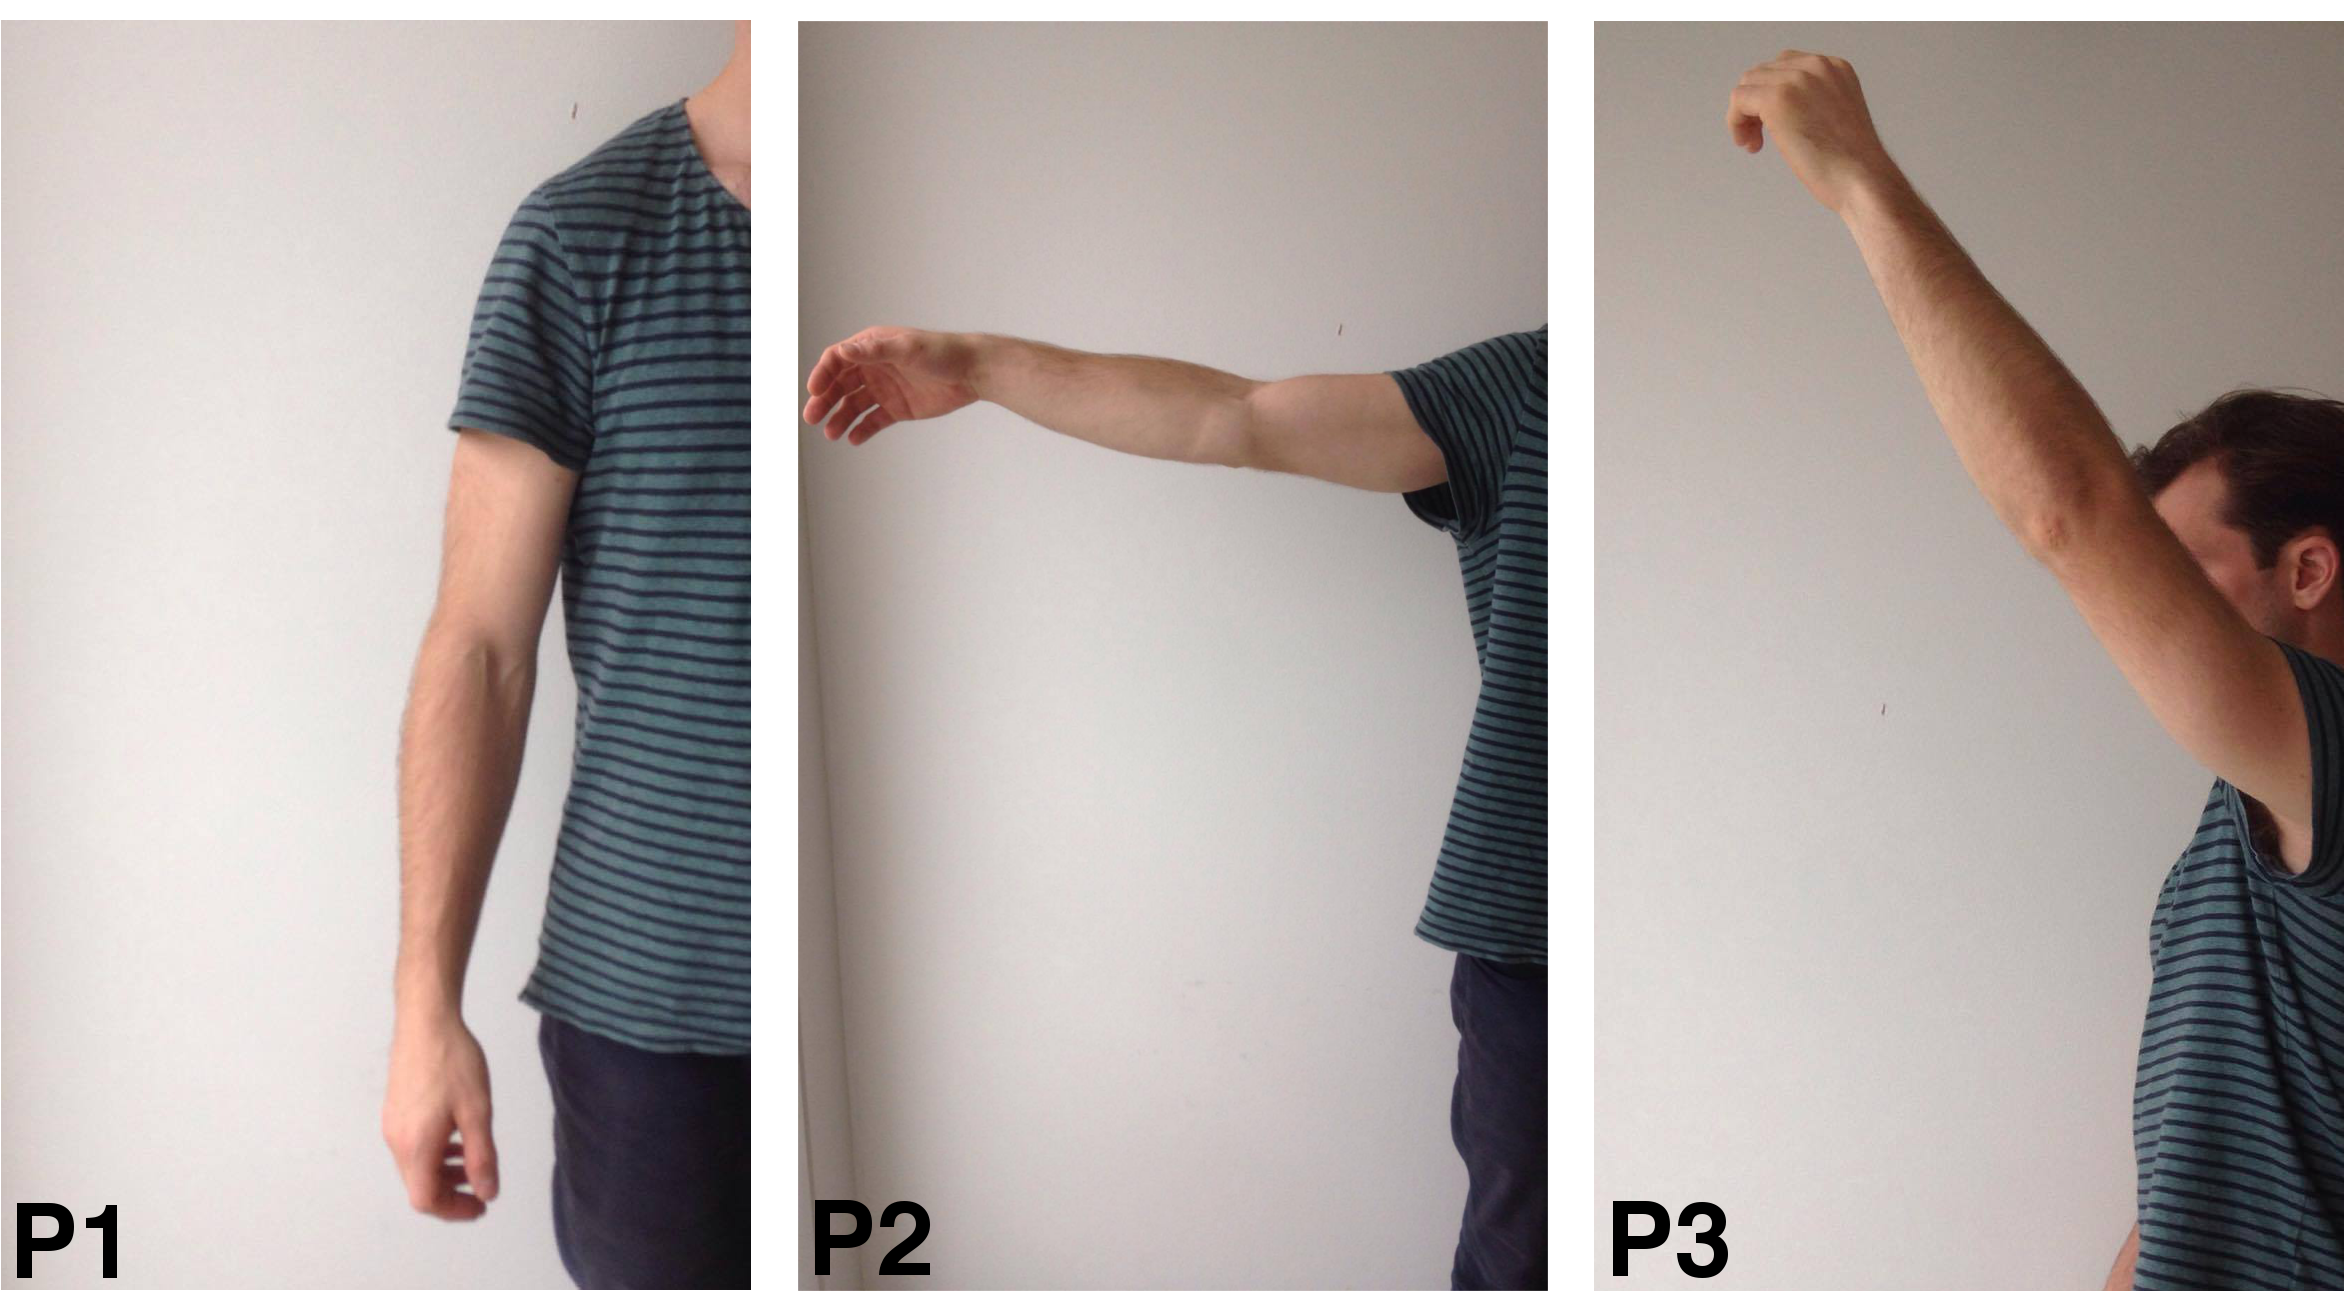
\includegraphics[width=0.4\textwidth]{figures/paperFigures/limb_pos}  %<--but is not needed.
	\caption{Illustration of the limb positions performed. P1: relaxed along the torso, P2: 90 degrees horizontally of the side of torso and P3: 135 degrees vertically in front of the torso}
	\label{fig:limbpositions}  %<--give the figure a label, so you can reference!
\end{figure}

\subsection{Feature extraction}
Features were extracted in a 200 ms window with a 50\% overlap, which is an acceptable segmentation for preserving information of the signal in static contractions \cite{Farfan2010}.
The commonly used Mean Absolute Value (MAV) feature was additionally extracted, and calculated as given by equation \ref{eq:mav}: \cite{Zecca2002} 

\begin{equation} \label{eq:mav}
MAV = \frac{1}{N}\sum\limits_{i=1}^N|x_i|
\end{equation}
where N is the length of the window, and $x_i$ is the EMG signal of $i$ samples.

MAV is directly correlated with change in EMG amplitude. No study has examined whether MAV contains linear properties, but EMG signals has heteroscedastic properties \cite{rasool2012} and the MAV feature might therefore not contain direct linear properties.

In a previous study \cite{hahne2014} it was shown that logarithmizing the variance of EMG the variance linearises, and has yielded robust control of wrist movements in a relaxed limb position when used in linear regression. The Logarithmic Variance (LogVar) was therefore extracted as a feature, and was calculated as given by equation \ref{eq:logvar}:

\begin{equation} \label{eq:logvar}
log(\sigma^2) = log(\frac{\sum\limits_{i=1}^N(x_i - \mu)^2}{N})
\end{equation}
where N expresses the length of the window, $x_i$ is the $i^{th}$ sample of the EMG signal and $\mu$ is the mean.

The Mean Value (MV) was extracted from the accelerometer data, similarly to a previous study \cite{Krasoulis2015} testing the effect of limb position using classification as control scheme. 

The extracted EMG features for the individual wrist movements were examined through a Principal Component Analysis, to evaluate, whether the different movements were distinguishable or new training data should be acquired.

\subsection{Regression model}
As applied in a study by Hwang et al. \cite{hwang2017} to achieve robust performance across variations in limb positions linear regression was used as control scheme. One regressor was trained for each wrist movement for both features; four regressors trained for each feature, and four for each feature where accelerometer data was included. Each regressor was trained based on multivariate linear regression and calculated as given by equation \ref{eq:linearregression}:

\begin{equation} \label{eq:linearregression}
\hat{Y} = \alpha + \beta_1 X_{1} + \beta_2 X_{2} + ... + \beta_i X_{i}
\end{equation}
where $\hat{Y}$ is the estimated value, $X_i$ are the predictors, $\beta_i$ are the regression coefficients in the sampled population, and $\alpha$ is the predicted value of $Y$ at $X_{i} = 0$. $\beta_i$ and $\alpha$ were fitted for each regressor using the extracted feature data for each channel as predictors. The mean of the absolute values of the actual EMG across all channels scaled in relation to the MVC is set as estimator values. The features for all wrist movements in all limb positions were included as predictors in the training of each regressor. However, only the desired wrist movement the regressor was fitted for, was trained with the actual estimated values. The remaining predictors were given 0 as estimated values. This procedure was applied for the regressors to more precisely recognize the performed movement.

\subsection{Offline testing}
The accuracy of the regressors was examined both qualitatively and quantitatively when using both training and test data. A qualitative test was performed by superimposing the regressor output on the actual data. The superimposition illustrated whether the right regressor reacted on the performed movement, and how accurate it responded compared to the actual data. For the quantitative analysis the Root Mean Square Error (RMSE) was calculated to compare through statistical analysis, which feature had the lowest error, and whether the regressors were overfitted when tested with new input data. Furthermore, the accuracy of the regressors trained with inclusion of accelerometer data were compared to the regressors trained only using EMG feature data. The RMSE was calculated as given by equation \ref{eq:rmse}:

\begin{equation} \label{eq:rmse}
RMSE = \sqrt{\frac{\sum\limits_{i=1}^N(y_i - \hat{y_i})^2}{N}}
\end{equation}
where N is the length of the window, $y_i$ is the $i^{th}$ variable of the actual data and $\hat{y_i}$ is the $i^{th}$ output of the regressor.

It was decided, which statistical analysis to apply, through a Kolmogorov-Smirnov test that assesses whether the data populations were normal distributed. An ANOVA test was applied if the data population belonged to a normal distribution, if not a Friedman's test was applied, which is the non-parametric correspondent to an ANOVA test.

\subsection{Online testing}
To investigate the effect of limb position in the regression control scheme an online virtual environment was developed, depicted in figure \ref{fig:targets}

\begin{figure}[H]
	\centering
	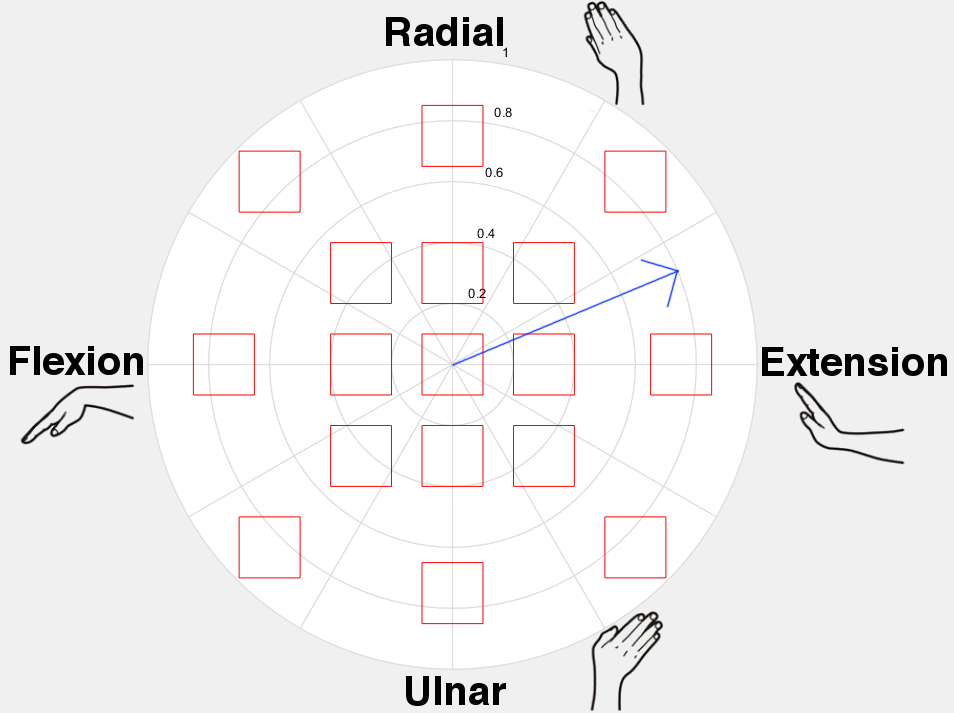
\includegraphics[scale=0.25]{figures/paperFigures/Target}
	\caption{A vector originated from origo depicted the EMG signal, where the length of the vector represented the EMG intensity, and direction was based on the movement performed. The wrist flexion-extension DOF was mapped to the x-axis, and the radial-ulnar deviation DOF was mapped to y-axis. The vector returned to the target located around origo when no contraction was made. For the subject to reach the targets in the diagonals, a simultaneous movement had to be performed. One target was shown at a time. When a target was reached, the vector had to return to the centred target for a new to appear. This gave the subject the same starting point when reaching each outer target. The procedure was performed until all targets had appeared. If a target was not reached within 30 s, it would disappear, and the vector had to return to the centred target.}
	\label{fig:targets}
\end{figure}

The time to complete a target-reaching task of sixteen targets was measured. 12 tests were performed by each subject; one in each limb position for each feature for the regressors trained with and without included accelerometer data. The performance score was calculated as the mean of time per reached target. Time to reach the centred target was not included in the performance score. Performance scores of the online test was compared between the different limb positions of the same feature, between all limb positions of the two features and between performance score obtained when using regressors trained with and without inclusion of accelerometer data. The same comparison was additionally applied for the amount of targets reached. The statistical analysis applied was again based on whether the populations were normal distributed or not. 

\newpage
\clearpage
\end{multicols}

\section{RESULTS}%%%%%%%%%%%%%%%%%%%%%%%%%%%%%%%%%%%%%%%%%%%%%%%%%%%%%%%%%%%%%%%%%%%

\begin{figure}[H]
	\centering
	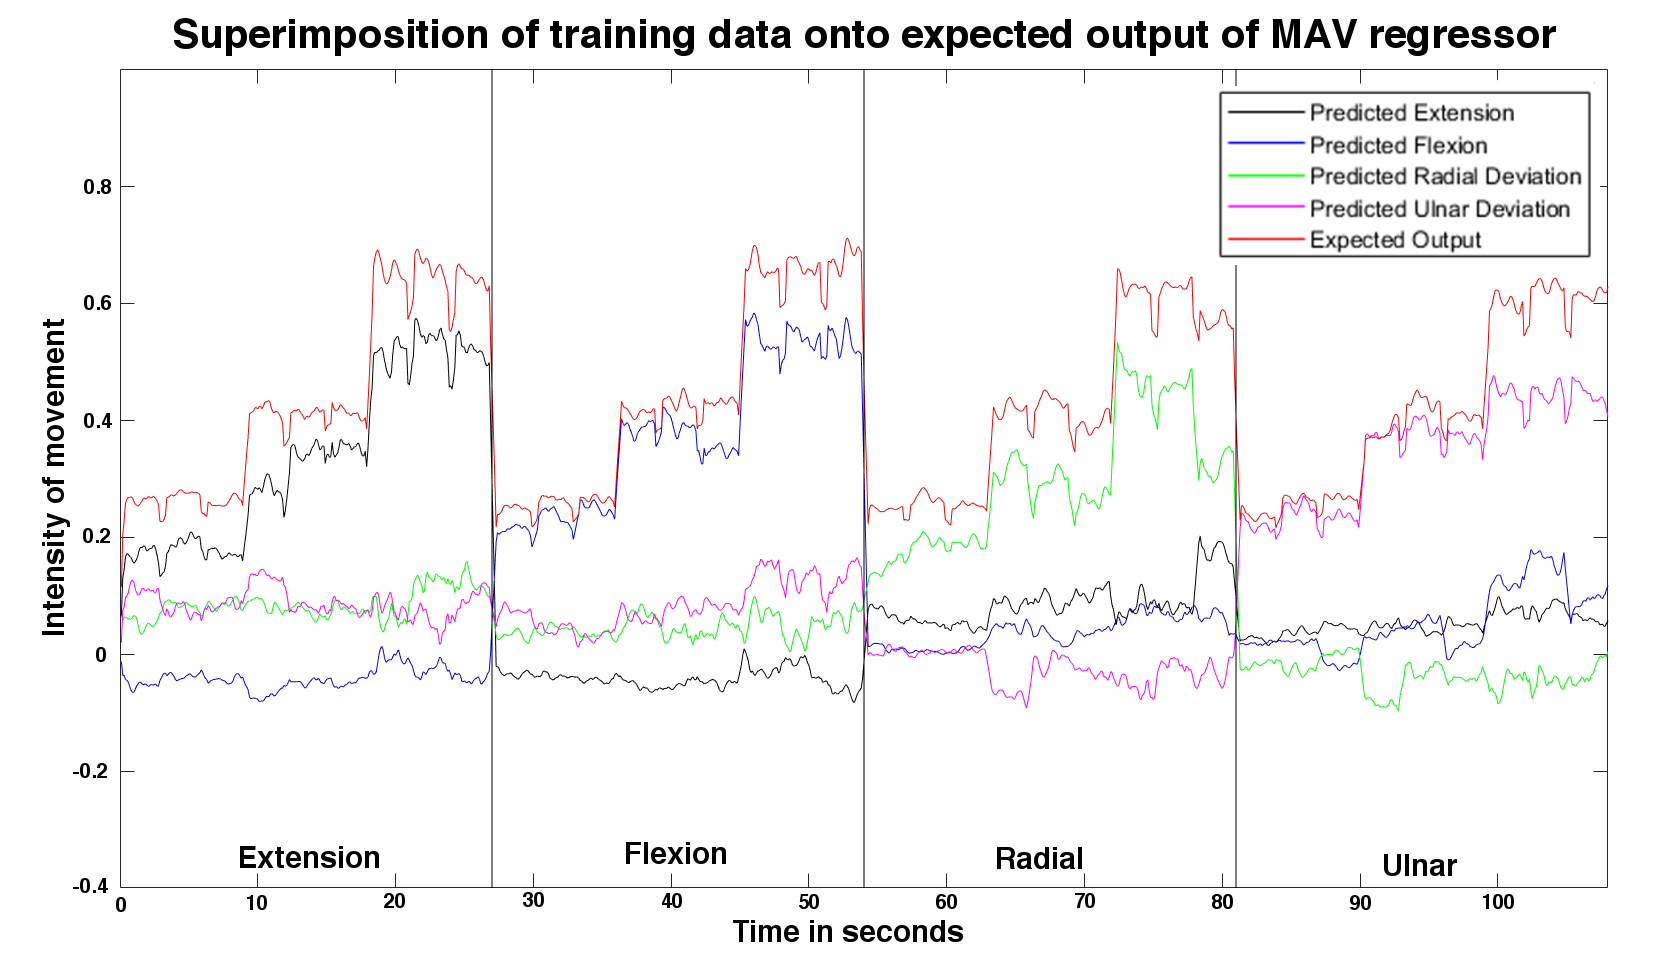
\includegraphics[width=0.6\textwidth]{figures/paperFigures/NewSuperPositionTestDataMAV}  %<--but is not needed.
	\caption{Plot of the actual data, red plot, superimposed on the output of the regressors trained with the MAV features. The plot is divided into four segments, where each segment shows a different movement performed. Each segment has the same sample size.}
	\label{fig:SuperPositionTrainingMAV}  %<--give the figure a label, so you can reference!
\end{figure}

\begin{figure}[H]
	\centering
	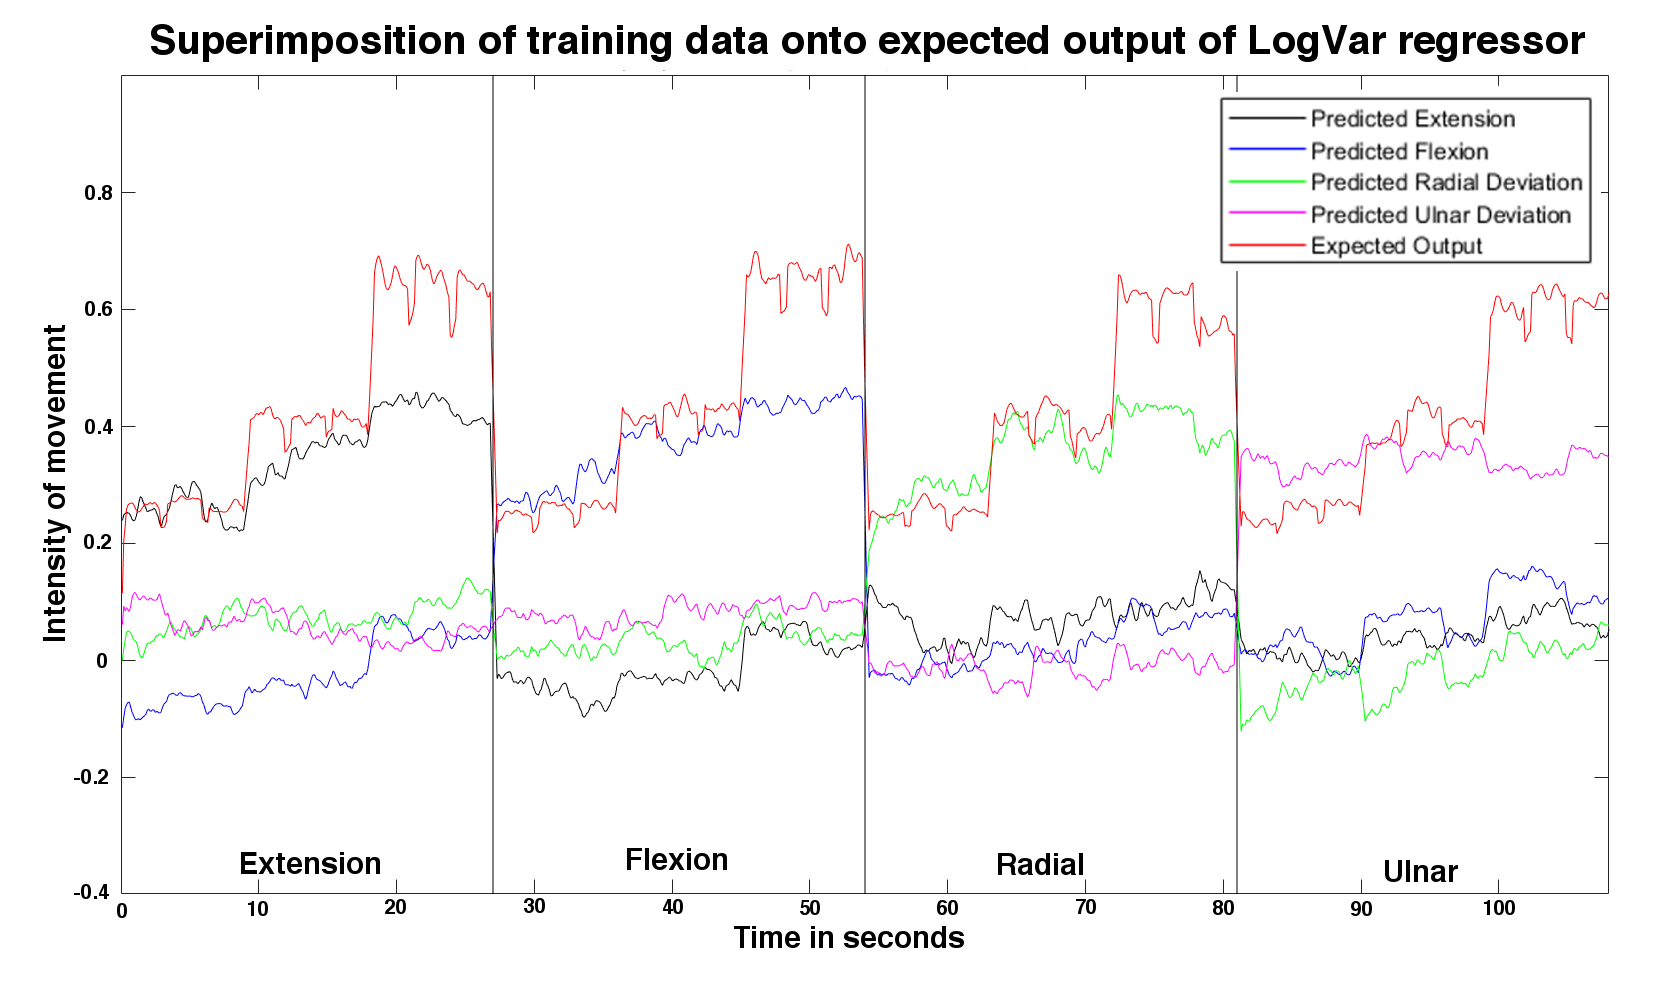
\includegraphics[width=0.6\textwidth]{figures/paperFigures/NewSuperPositionTestDataLogVar}  %<--but is not needed.
	\caption{Plot of the actual data, red plot, superimposed on the output of the regressors trained with the LogVar features. The plot is divided into four segments, where each segment shows a different movement performed. Each segment has the same sample size.}
	\label{fig:SuperPositionTrainingLogVar}  %<--give the figure a label, so you can reference!
\end{figure}

\begin{figure}[H]
	\centering
	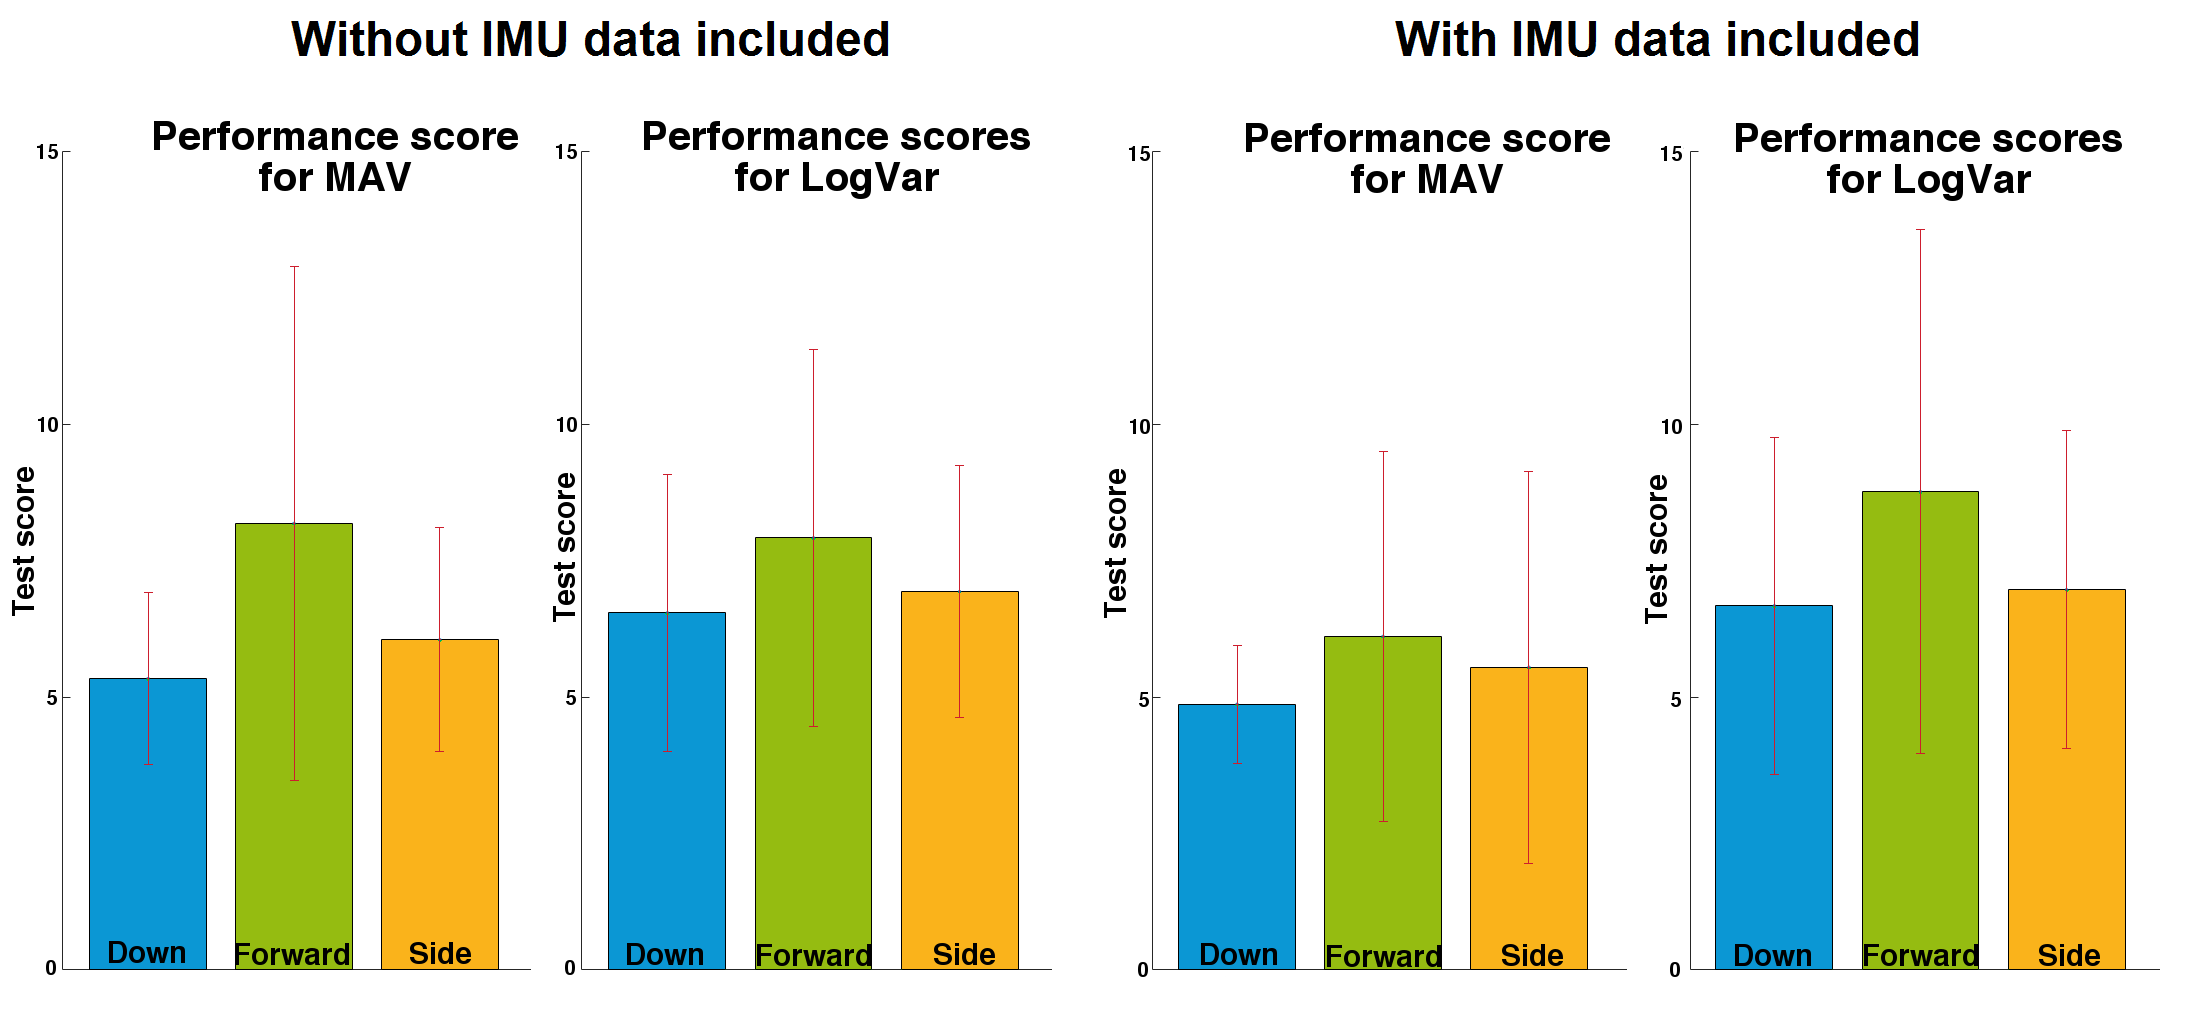
\includegraphics[width=0.4\textwidth]{figures/paperFigures/GotItTimeCol}  %<--but is not needed.
	\caption{Plot of the actual data, red plot, superimposed on the output of the regressors trained with the MAV features. The plot is divided into four segments, where each segment shows a different movement performed. Each segment has the same sample size.}
	\label{fig:GotItTimeCol}  %<--give the figure a label, so you can reference!
\end{figure}
	
\begin{figure}[H]
	\centering
	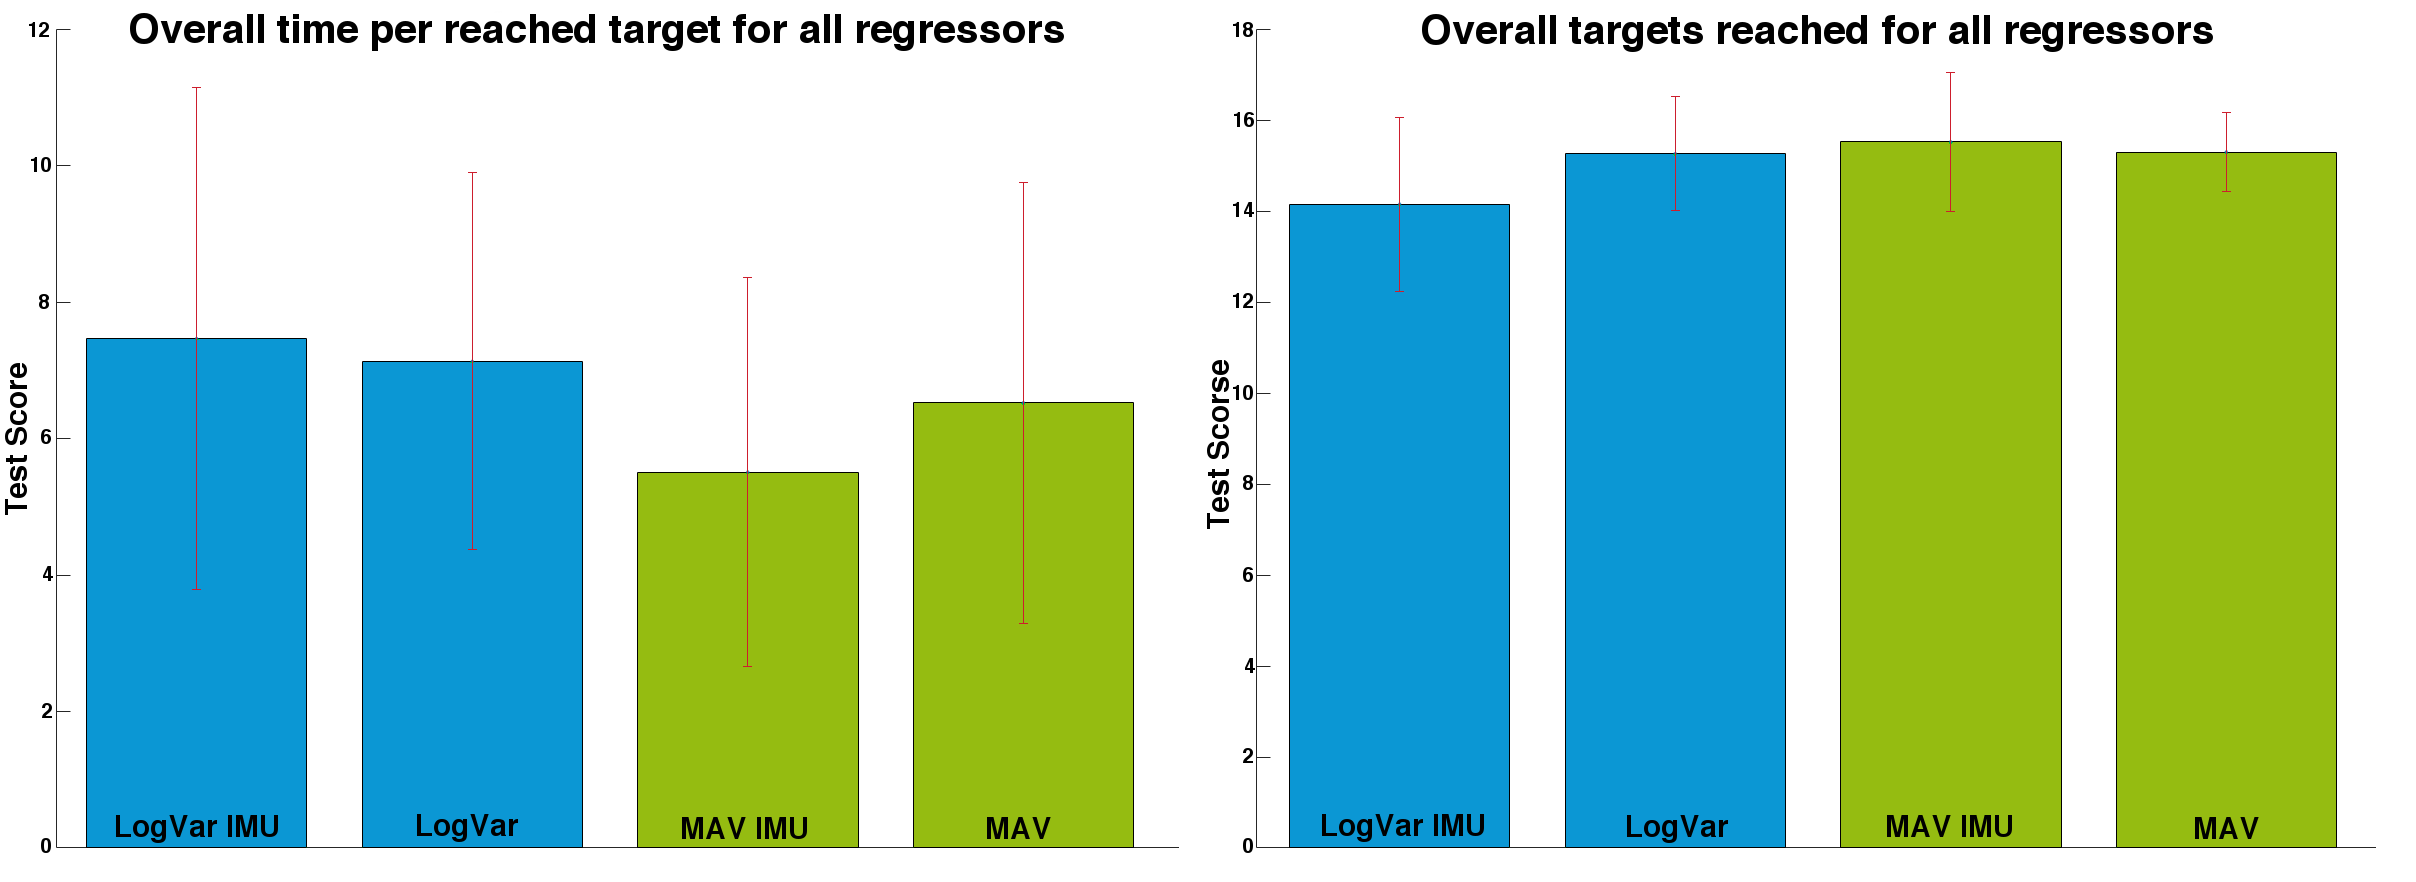
\includegraphics[width=0.4\textwidth]{figures/paperFigures/allRegressorBarzTimeScoreForTargetTestCol}  %<--but is not needed.
	\caption{Plot of the actual data, red plot, superimposed on the output of the regressors trained with the MAV features. The plot is divided into four segments, where each segment shows a different movement performed. Each segment has the same sample size.}
	\label{fig:TargetScoresTargetsCol}  %<--give the figure a label, so you can reference!
\end{figure}
	
\begin{multicols}{2}
	\begin{table}[H]
		\begin{center}
			\begin{tabular}{l l l}
				\hline
				\textbf{Feature} & \textbf{Overall mean error} & \textbf{Standard deviation}\\
				\hline
				Extension & 0.1030 & $\pm 0.0210$ \\
				Flexion & 0.1102 & $\pm 0.0296$ \\
				Radial Deviation & 0.1206 & $\pm 0.0298$ \\
				Ulnar Deviation & 0.1143 & $\pm 0.0334$ \\
				Overall & 0.1059 & $\pm 0.0306$ \\
				\hline
			\end{tabular}
			\caption{RMSE for the implemented MAV regressor}
		\end{center}
	\end{table}
	
	\begin{table}[H]
		\begin{center}
			\begin{tabular}{l l l}
				\hline
				\textbf{Feature} & \textbf{Overall mean error} & \textbf{Standard deviation}\\
				\hline
				Extension & 0.1157 & $\pm 0.0469$ \\
				Flexion & 0.1102 & $\pm 0.0241$ \\
				Radial Deviation & 0.1142 & $\pm 0.0256$ \\
				Ulnar Deviation & 0.1312 & $\pm 0.0310$ \\
				Overall & 0.1178 & $\pm 0.0272$ \\
				\hline
			\end{tabular}
			\caption{RMSE for the implemented LogVar regressor}
		\end{center}
	\end{table}
	
	Analysing the RMSE of the regression models' response to the training data, it was found that there's a significant difference (p = 0.0044) between MAV and LogVar, where it was shown that LogVar (mean = 0.1178, std = 0.0272) has a higher mean than MAV (mean = 0.0159, std = 0.0306).
	
	\begin{table}[H]
		\begin{center}
			\begin{tabular}{l l l}
				\hline
				\textbf{Feature} & \textbf{Overall mean error} & \textbf{Standard deviation}\\
				\hline
				Extension & 0.1646 & $\pm 0.0753$ \\
				Flexion & 0.1391 & $\pm 0.0841$ \\
				Radial Deviation & 0.2018 & $\pm 0.0424$ \\
				Ulnar Deviation & 0.1743 & $\pm 0.0905$ \\
				Overall & 0.1700 & $\pm 0.0759$ \\
				\hline
			\end{tabular}
			\caption{RMSE for the implemented MAV regressor}
		\end{center}
	\end{table}
	
	
	\begin{table}[H]
		\begin{center}
			\begin{tabular}{l l l}
				\hline
				\textbf{Feature} & \textbf{Overall mean error} & \textbf{Standard deviation}\\
				\hline
				Extension & 0.1552 & $\pm 0.0514$ \\
				Flexion & 0.1680 & $\pm 0.0508$ \\
				Radial Deviation & 0.1681 & $\pm 0.0540$ \\
				Ulnar Deviation & 0.2078 & $\pm 0.0621$ \\
				Overall & 0.1748 & $\pm 0.0563$ \\
				\hline
			\end{tabular}
			\caption{RMSE for the implemented LogVar regressor}
		\end{center}
	\end{table}
	
	\begin{table}[H]
		\begin{center}
			\begin{tabular}{l l}
				\hline
				\textbf{Compared features} & \textbf{P-Value}\\
				\hline
				LogVar, MAV & 0.0044 \\
				LogVar test data, MAV test data & 0.1138 \\
				LogVar test data, LogVar & 0.0001 \\
				MAV test data, MAV & 0.000002 \\
				\hline
			\end{tabular}
			\caption{P-Values for comparison of the features}
		\end{center}
	\end{table}
	
	It was found that there is a significant difference (p = 0.0001) between the RMSE for test data (mean = 0.1748, std = 0.0563) and training data (mean = 0.1178, std = 0.0272) for LogVar. A significant difference (p = 0.000002) was also found for the test data (mean = 0.1700, std = 0.0759) and training data (mean = 0.1059, std = 0.0306) for the MAV based regression models. No significant difference (p = 0.1138) was found between MAV (mean = 0.1700, std = 0.0759) and LogVar (mean = 0.1748, std = 0.0563) regression models with test data.
	
	\begin{table}![H]
		\begin{center}
			\begin{tabular}{l l l}
				\hline
				\textbf{Limb position, feature} & \textbf{Overall mean error} & \textbf{Standard deviation}\\
				\hline
				Down, MAV & 5.3377 & $\pm 1.5696$ \\
				Forward, MAV & 8.1791 & $\pm 4.7145$ \\
				Side, MAV & 6.0490 & $\pm 2.0490$ \\
				Down, LogVar & 6.5404 & $\pm 2.5315$ \\
				Forward, LogVar & 7.9123 & $\pm 3.4572$ \\
				Side, LogVar & 6.9325 & $\pm 2.3036$ \\
				\hline
			\end{tabular}
			\caption{Test scores for the different limb for MAV and LogVar regressors}
		\end{center}
	\end{table}
	\begin{table}[H]
		\begin{center}
			\begin{tabular}{l l}
				\hline
				\textbf{Feature} & \textbf{P-Value}\\
				\hline
				MAV & 0.8948 \\
				LogVar & 0.2359 \\
				\hline
			\end{tabular}
			\caption{P-Values for comparison of the score in different limb positions with MAV and LogVar}
		\end{center}
	\end{table}
	
	When comparing the score for different limb positions, no significant difference was found for either MAV (p = 0.8948) or LogVar (p = 0.2359).
	
	\begin{table}[H]
		\begin{center}
			\begin{tabular}{l l l}
				\hline
				\textbf{Limb position, feature} & \textbf{Overall mean error} & \textbf{Standard deviation}\\
				\hline
				Down, MAV & 15.5556 & $\pm 0.7265$ \\
				Forward, MAV & 15.1111 & $\pm 1.0541$ \\
				Side, MAV & 15.2222 & $\pm 0.8333$ \\
				Down, LogVar & 15.4444 & $\pm 0.7265$ \\
				Forward, LogVar & 15 & $\pm 1.8020$ \\
				Side, LogVar & 15.3333 & $\pm 1.1180$ \\
				\hline
			\end{tabular}
			\caption{Targets reached in the target test with the MAV and LogVar regressors.}
		\end{center}
	\end{table}
	
	\begin{table}[H]
		\begin{center}
			\begin{tabular}{l l}
				\hline
				\textbf{Feature} & \textbf{P-Value}\\
				\hline
				MAV & 0.0212 \\
				LogVar & 0.4220 \\
				\hline
			\end{tabular}
			\caption{P-Values for comparison of the number of reached targets in different limb positions with MAV and LogVar}
		\end{center}
	\end{table}
	
	It was shown that there is a significant difference (p = 0.0212) between the number of targets reached in the different positions for MAV, where the limb pointed forward yielded worst results (mean = 15.1111, std = 1.0541). No significant difference (p = 0.4220) was found between the limb positions for LogVar.
	
	
	
	\begin{table}[H]
		\begin{center}
			\begin{tabular}{l l l}
				\hline
				\textbf{Limb position,feature} & \textbf{Overall mean error} & \textbf{Standard deviation}\\
				\hline
				Down, MAV & 4.8661 & $\pm 1.0839$ \\
				Forward, MAV & 6.1094 & $\pm 3.3852$ \\
				Side, MAV & 5.5442 & $\pm 3.5847$ \\
				Down, LogVar & 6.6691 & $\pm 3.0798$ \\
				Forward, LogVar & 8.7595 & $\pm 4.7969$ \\
				Side, LogVar & 6.9652 & $\pm 2.9144$ \\
				\hline
			\end{tabular}
			\caption{Test scores for the different limb for MAV and LogVar regressors with IMU included.}
		\end{center}
	\end{table}
	
	\begin{table}[H]	
		\begin{center}
			\begin{tabular}{l l}
				\hline
				\textbf{Feature} & \textbf{P-Value}\\
				\hline
				MAV & 0.0319 \\
				LogVar & 0.4594 \\
				\hline
			\end{tabular}
			\caption{P-Values for comparison of the score in different limb positions with MAV and LogVar with IMU data included}
		\end{center}
	\end{table}
	
	A significant difference (p = 0.0319) was found between the test score in different limb positions for MAV with IMU included, where the worst performance was found with the arm pointed forward (mean = 6.1094, std = 3.3852). No significant difference (p = 0.4594) was found between limb positions for the LogVar regression model with IMU data included.
	
	\begin{table}[H]
		\begin{center}
			\begin{tabular}{l l l}
				\hline
				\textbf{Limb position,feature} & \textbf{Overall mean error} & \textbf{Standard deviation}\\
				\hline
				Down, MAV & 15.8889 & $\pm 0.3333$ \\
				Forward, MAV & 15.1111 & $\pm 2.3154$ \\
				Side, MAV & 15.5556 & $\pm 1.3333$ \\
				Down, LogVar & 14.7778 & $\pm 1.7159$ \\
				Forward, LogVar & 13.5556 & $\pm 2.1858$ \\
				Side, LogVar & 14.1111 & $\pm 1.8333$ \\
				\hline
			\end{tabular}
			\caption{RMSE for the implemented LogVar regressor}
		\end{center}
	\end{table}
	
	\begin{table}[H]
		\begin{center}
			\begin{tabular}{l l}
				\hline
				\textbf{Compared Features} & \textbf{P-Value}\\
				\hline
				MAV & 0.2957 \\
				LogVar & 0.0037 \\
				\hline
			\end{tabular}
			\caption{P-Values for comparison of the number of targets reached in different limb positions with MAV and LogVar with IMU data included}
		\end{center}
	\end{table}
	
	There was no significant difference found for the MAV regressor with IMU data included (p = 0.2957). The number of targets reached in different limb positions was proven significantly different (p = 0.0037) for the LogVar feature with IMU data included, where the lowest number of targets reached was found with the arm pointed forward (mean = 13.5556, std = 2.1858).
	
	
	\begin{table}[H]
		\begin{center}
			\begin{tabular}{l l l}
				\hline
				\textbf{Feature} & \textbf{Mean score} & \textbf{Standard deviation}\\
				\hline
				MAV & 6.5219 & $\pm 3.2253$ \\
				MAV w. IMU & 5.5066 & $\pm 2.8477$ \\
				LogVar & 7.1284 & $\pm 2.7619$ \\
				LogVar w. IMU & 7.4646 & $\pm 3.6740$ \\
				\hline
			\end{tabular}
			\caption{Average score of the target test for the four regressor designs}
		\end{center}
	\end{table}
	
	\begin{table}[H]
		\begin{center}
			\begin{tabular}{l l}
				\hline
				\textbf{Compared features} & \textbf{P-Value}\\
				\hline
				LogVar w/ IMU, MAV w/ IMU & 0.5637 \\
				LogVar, MAV & 0.0833 \\
				LogVar w/ IMU, LogVar & 0.5637 \\
				MAV w/ IMU, MAV & 0.1779 \\
				\hline
			\end{tabular}
			\caption{P-Values for comparison of the overall scores of the target tests}
		\end{center}
	\end{table}
	
	A significant difference (p = 0.5637) could not be proven between the scores of the target test for LogVar with IMU data and MAV with IMU data. There was no significant difference (p = 0.0833) between the score of LogVar without IMU data and MAV without IMU data. It was also found that there is no significant difference between regression models with and without IMU data for both MAV (p = 0.1179) and LogVar (p = 0.5637).	
	
	\begin{table}[H]
		\begin{center}
			\begin{tabular}{l l l}
				\hline
				\textbf{Feature} & \textbf{Overall mean error} & \textbf{Standard deviation}\\
				\hline
				MAV & 15.2963 & $\pm 0.8689$ \\
				MAV w/ IMU & 15.5185 & $\pm 1.5285$ \\
				LogVar & 15.2593 & $\pm 1.2586$ \\
				LogVar w/ IMU & 14.1481 & $\pm 1.9156$ \\
				\hline
			\end{tabular}
			\caption{Average number of targets reached in the target test for the four regressor designs}
		\end{center}
	\end{table}
	
	\begin{table}[H]
		\begin{center}
			\begin{tabular}{l l}
				\hline
				\textbf{Compared Features} & \textbf{P-Value}\\
				\hline
				LogVar w/ IMU, MAV w/ IMU & 0.0017 \\
				LogVar, MAV & 1 \\
				LogVar w/ IMU, LogVar & 0.0016 \\
				MAV w/ IMU, MAV & 0.0124 \\
				\hline
			\end{tabular}
			\caption{P-Values for comparison targets reached in the target tests}
		\end{center}
	\end{table}
	
	A significant difference (p = 0.0017) was found between targets reached when IMU was included, where LogVar (mean = 14.1481, std = 1.9156) was proven worse than MAV (mean = 15.5185, std = 1.5285). There was a significant difference (p = 0.0016) between LogVar with (mean = 14.1481, std = 1.9156) and without (mean = 15.2593, std = 1.2586) IMU data. The same significant difference (p = 0.0124) between MAV with (mean = 15.5185, std = 1.5285) and without (mean = 15.2963, std = 0.8689) IMU data. There was no difference (p = 1) between targets reached with LogVar and MAV when IMU was not included.
	
\section{DISCUSSION}%%%%%%%%%%%%%%%%%%%%%%%%%%%%%%%%%%%%%%%%%%%%%%%%%%%%%%%%%%%%%%%%
	
%		%discussion points
The present paper had as porpuose to study the performance of linear regression methods for myoelectric prostheses control taking in acount the limb position effect. Along the process different aspects have been exposed that are important to mention.\\
%subdivide in sections??
%Potential outliers were discoverd during this study. Even though the final results present that is possible to achieve simultaneous and proportional control using Myo armband, it had been shown that the sampling rate of this device could affect the acquisition of sEMG data. This could be due to the fact that sEMG signals  rate is between 10-500Hz, however the sampling rate of the Myoarmband is 200Hz, which casuses important information in raw data to be eliminated.
%Based on prevoius studies two different features were extracted in order to tran the regressors MAV and LogVar.
%A study by Hanhe \cite{hanhe2014} et al. showed that LogVar presented linear properties and outperformed the other different features extracted for that particular research. However the obtained results in our study illustrates that MAV performance outperformed the LogVar results. 
%Futhermore online results were not siginificant different depending on the limb position as other studies had shown for classification control scheme. This findings agree with a recently published study by Hwang et al. \cite{Hwang2017}. In their study different limb position were tested using Root Mean Square (RMS) as feature to train the regressors.
%During the results examination it was found that there is no correlation between the offline and online results. On the one hand the offline outcomes illustrates overfitting of the regression models. On the other hand the online test yielded robust control of the wrist movements performanced in the three different limb positions. This could be owing to the subjects$'$ ability to compensate for a poorer fitting model when visual feedback is provided.
%It have been proved that is possible to achieve simultaneous and proportional control in myoelectric prosthesis using linear regression techniques. 
%\begin{itemize}
	%\item inclusion of more subjects
%	\item sample rate of the myo armband - exclusion of test subjects
	%\item even though LogVar shows linearity in a previous study, it does not perform better in linear regression than a presumably non-linear feature
	%\item Both features does not show significant difference in control in different limb positions
%	\item Whatever the inclusion of IMU shows 
	
%	\item It is possible to use regression as control method to yield no significantly different performance in variations of limb positions
	%\item Use other regression methods and other features to analyse if it will result in better performance
	%\item why does the inclusion of IMU improve the performance
%	\item No connection between offline and online tests, which also is shown in previous studies
%	\item reasonable control can be archived when donning/doffing(we train the regressors with data, take of the myo armband, and do the testing with the myo armband placed slightly elsewhere)
	
%\end{itemize}
	\subsection{Offline and online training}
	Offline and online training was done for both MAV and LogVar without IMU data included, with a significant difference between the two features when testing with training data (p = 0.0044) but no difference when testing with new data (p = 0.1138). Overall it was found that there were no apparent correlation between offline and online testing. This could be caused by the subjects ability to adjust to a poor fitted model when given the visual feedback while performing the target test. This finding corresponds to the findings in other studies \cite{jiang2010}.
	
	\subsection{Comparison of features}
	In the results it was found that there was no significant difference between the performance of LogVar and MAV when it comes to the scores for the target test both with (p = 0.5637) and without (p = 0.0833) IMU data included. Based on previous studies showing LogVar as a feature with linear properties, it would be expected that this feature would perform better in a linear regression model, than a feature which to the authors knowledge has not been proven to be linear. On the contrary it was shown that a significantly higher number of targets was reached with a linear regression models based on the MAV feature with IMU included, compared to the LogVar regression model with IMU included (p = 0.0017). When IMU data wasn't included, there was no difference between the number of targets reached in the test (p = 1).
	
	Further studies within this field should consider examining other features, while studying the effect of combining several features in order to yield better performance independent of the limb position.
	
	\subsection{Inclusion of IMU data}
	The IMU data included in this study was based on a single accelerometer, where it was expected that the Myo band would give a similar output as long as the subjects were performing both training and testing from the same starting position. Inclusion of the IMU data was shown to yield the same results when it comes to the test score, with no significant difference for either MAV (p = 0.1779) or LogVar (p = 0.5637) when comparing regression models build with and without accelerometer inputs. It was found that the inclusion of the IMU data yielded significantly worse results for the LogVar regression model (p = 0.0016), while it led to a significant improvement of the MAV regression model (p = 0.0124) when examining the number of reached targets. The inclusion of IMU data could be a subject of further investigation, as the results might be improved by implementing a system capable of measuring the angles of the joints, in order to create a more versatile and usable regression model outside the clinical environment.  
	
	\subsection{Stability in limb positions}
	When excluding IMU data, there was no significant difference between the target score for either LogVar (p = 0.2359) or MAV (p = 0.8948) in the different limb positions, while there was a difference between the number of reached targets for MAV (0.0212) but no difference for LogVar (p = 0.4220). This outcome shows that both MAV and LogVar yields rather stable performance in different limb positions when used to create linear regression based control schemes.
	
	When including IMU data the MAV based regression model was shown to have a significant difference between the score of different limb positions (p = 0.0319), while LogVar did not show any difference (p = 0.4594). While the time taken to reach targets were shown to be different depending on limb positions when using MAV, the number of targets reached was improved, so that the number of reached targets with MAV were not shown to be significantly different (p = 0.2957). The LogVar feature based regression models were shown to have a difference between reached targets when using IMU data (p = 0.0037).
	
	Overall the LogVar regression models were observed as being the most unstable in the different limb positions when looking at the test subjects performance in the target test. This might be a result of the LogVar feature being based on the change of the signal, as this could lead to problems with crosstalk when the arm is not in a relaxed state. The MAV was observed as being more stable, with the subjects being able to create more controlled movements as well as having the possibility to adjust the position of the arrow when trying to get back to the middle of the test GUI. Based on the findings of this study, it would be recommended to examine features based on the amplitude rather than the variance in future studies within this area.
	
	\subsection{Limitations of the study}
	This study was based on data from 12 test subjects, where three had to be excluded. One subject was excluded due to misunderstanding the given instructions and thereby creating an unusable set of training and test data, which limited the control of the regression models giving him a mean score above 25 seconds per target and average number of reached targets below 10 for all tests.
	
	Two other subjects were excluded as the recorded intensities were not high enough to differ between the baseline and the intended movement. This caused the regression models to interpret the baseline in the target test as movements being performed at between 30\% and 70\% of the MVC.
	
	To improve the validity of the study more test subjects should be included in further studies within this field. Subjects with transradial amputations should also be taken into consideration if the regression based control schemes were to be considered for future use in myoelectric prosthetic devices. 
	
	Using the Myo band for data acquisition led to certain limitations in the sample rate, as the device is only capable of recording signals between 0 and 200Hz. This leads to the final signal being recorded between 0 and 100Hz, where everything above 100Hz is affected by aliasing. Along with frequency limitations, the Myo band restricted the number and placement of electrodes to eight channels placed at the same distance from the elbow, where it might be possible to yield better results with a different electrode placement and number. Further studies should implement regular EMG electrodes in order to obtain a more usable and clear signal, that represents the entire frequency band of EMG signals.
	
	
%	\begin{table}[h]
%		\caption{An Example of a Table}
%		\label{table_example}
%		\begin{center}
%			\begin{tabular}{|c||c|}
%				\hline
%				One & Two\\
%				\hline
%				Three & Four\\
%				\hline
%			\end{tabular}
%		\end{center}
%	\end{table}
	


	
	
	%Figure Labels: Use 8 point Times New Roman for Figure labels. Use words rather than symbols or abbreviations when writing Figure axis labels to avoid confusing the reader. As an example, write the quantity ÒMagnetizationÓ, or ÒMagnetization, MÓ, not just ÒMÓ. If including units in the label, present them within parentheses. Do not label axes only with units. In the example, write ÒMagnetization (A/m)Ó or ÒMagnetization {A[m(1)]}Ó, not just ÒA/mÓ. Do not label axes with a ratio of quantities and units. For example, write ÒTemperature (K)Ó, not ÒTemperature/K.Ó
\textbf{Comparison of features.}
The online results indicated no significant difference between LogVar and MAV in the performance scores both with (p = 0.5637) and without (p = 0.0833) IMU data included. Based on a study \cite{hahne2014} showing LogVar as a feature with linear properties, it would be expected that this feature would perform better in a linear regression model, than a feature which to the authors knowledge has not been proven to be linear. On the contrary it was shown that a significantly higher number of targets was reached with a linear regression models based on the MAV feature with IMU included, compared to the LogVar regression model with IMU included (p = 0.0017). When IMU data was not included, there was no difference between the number of targets reached in the test (p = 1).

Further studies within this field should consider examining other features and studying the effect of combining several features in order to further improve performance independent of the limb position.

\textbf{Inclusion of IMU data.}
The IMU data included in this study was based on a single accelerometer, where it was expected that the Myo armband would give a similar output as long as the subjects were performing both training and testing from the same starting position. Inclusion of the IMU data was shown to yield the same results in the online test scores, with no significant difference for either MAV (p = 0.1779) or LogVar (p = 0.5637) when comparing regression models trained with and without accelerometer inputs. Inclusion of the IMU data yielded significantly poorer results for the LogVar regression model (p = 0.0016), while it led to a significant improvement of the MAV regression model (p = 0.0124) when examining the number of reached targets. The inclusion of IMU data could be a subject of further investigation, as the results might be improved by implementing a system capable of measuring the angles of the joints, in order to create a more versatile and usable regression model outside the clinical environment. Including IMU data could additionally be used to select specific regression models, if a system was build with models fitted for each limb position instead of the same regressors for all positions. 

\textbf{Stability in limb positions.}
When excluding IMU data, there was no significant difference between the performance score for either LogVar (p = 0.2359) or MAV (p = 0.8948) in the different limb positions, while there was a difference between the number of reached targets for MAV (0.0212) but no difference for LogVar (p = 0.4220). This outcome shows that both MAV and LogVar yields stable performance in different limb positions in a linear regression-based control scheme. This finding agrees with Hwang et al. \cite{Hwang2017}, who equivalently found stable online performance across limb positions in a linear regression-based control scheme applying RMS as feature.

When including IMU data the MAV based regression model was shown to have a significant difference in scores between limb positions (p = 0.0319), while LogVar did not (p = 0.4594). While the target reaching time were shown to be different depending on limb positions when using MAV, the number of targets reached was improved, as there was no significant difference (p = 0.2957) in the amount of targets reached. The LogVar feature based regression models were shown to have a difference between reached targets when using IMU data (p = 0.0037).

Overall the LogVar regression models were observed as being the most unstable in the different limb positions when examining the test subjects performance in the target-reaching test. This might be a result of the LogVar feature being based on the change of the signal, as this could lead to problems with crosstalk, when the arm is not in a relaxed state. MAV was observed as being more stable, with the subjects being able to create more smooth movements as well as being able to controllably return to the resting position. Based on the findings of this study, it would be recommended to examine features based on the amplitude rather than the variance in future studies within this area.

\textbf{Offline vs. online training.}
Offline testing was only done for MAV and LogVar without IMU data included. A significant difference between the two features when testing with training data (p = 0.0044) was archived in the offline test, but no significant difference when testing with new data (p = 0.1138). Comparing RMSE of LogVar with training data and RMSE of LogVar with new data there was a significant difference (P = 0.0001), where RMSE of the test with new data has the higher mean. Same results were yielded for the MAV trained regressors (P = 0.000005). This indicates that the regression models were overfitted when exposed to new data. The online results yielded robost control across all limb positions, and therefore no apparent correlation between offline and online testing. This could be caused by the subjects ability to adjust to a poor fitted model when given visual feedback while performing the target-reaching test. This observation corresponds to findings in another study \cite{jiang2010}.

\textbf{Limitations of the study.}
This study was based on data from 12 test subjects, where three had to be excluded. One subject was excluded due to misunderstanding the given instructions and thereby creating an unusable set of training and test data. This limited the control of the regression models giving the subject a mean score above 25 s per target reached and average number of reached targets below 10 for all tests.

Two other subjects were excluded as the recorded intensities were not high enough to differ between the baseline and the higher EMG intensity. This caused the regression models to interpret the baseline in the target-reaching test as movements being performed at between 30\% and 70\% of the MVC. 

To improve the validity of the findings more test subjects should be included in future studies within this field. Subjects with transradial amputations should also be taken into consideration if regression based control schemes were to be considered for future use in myoelectric prosthetic devices. 

Using the Myo armband for data acquisition limited the sampling rate to 200 Hz. Only the 0-100 Hz spectrum of the EMG was represented correctly, where frequencies above 100 Hz was affected by aliasing. Along with frequency representation limitations, the Myo armband restricted the number and placement of electrodes to eight channels placed at the same distance distal to the elbow joint, where it might be possible to yield better results with a different electrode placement and number of channels. Further studies should implement conventional EMG electrodes and an ADC with a sufficient sample rate, enabling the entire frequency band of EMG signals to be acquired correctly.		
	
\section{CONCLUSIONS}%%%%%%%%%%%%%%%%%%%%%%%%%%%%%%%%%%%%%%%%%%%%%%%%%%%%%%%%%%%%%%%
	
% 		Linear regression methods were applied for the two different features extracted. We compared both performance, training the regressor with EMG data as well as a combination of EMG data and IMU data.
	
	\addtolength{\textheight}{-12cm}   % This command serves to balance the column lengths
	% on the last page of the document manually. It shortens
	% the textheight of the last page by a suitable amount.
	% This command does not take effect until the next page
	% so it should come on the page before the last. Make
	% sure that you do not shorten the textheight too much.
In conclusion linear regression can be implemented as control scheme in myoelectric prosthetic control to yield performance with no significant difference across variations of limb position. This is opposed to previous studies using classification as control scheme.
 		
	
	%%%%%%%%%%%%%%%%%%%%%%%%%%%%%%%%%%%%%%%%%%%%%%%%%%%%%%%%%%%%%%%%%%%%%%%%%%%%%%%%
	
	
	
	%%%%%%%%%%%%%%%%%%%%%%%%%%%%%%%%%%%%%%%%%%%%%%%%%%%%%%%%%%%%%%%%%%%%%%%%%%%%%%%%
	
	
	
	%%%%%%%%%%%%%%%%%%%%%%%%%%%%%%%%%%%%%%%%%%%%%%%%%%%%%%%%%%%%%%%%%%%%%%%%%%%%%%%%
	\section*{APPENDIX}
	
	Appendixes should appear before the acknowledgment.
	
	\section*{ACKNOWLEDGMENT}
	
	The preferred spelling of the word ÒacknowledgmentÓ in America is without an ÒeÓ after the ÒgÓ. Avoid the stilted expression, ÒOne of us (R. B. G.) thanks . . .Ó  Instead, try ÒR. B. G. thanksÓ. Put sponsor acknowledgments in the unnumbered footnote on the first page.
	
\end{multicols}
	
	%%%%%%%%%%%%%%%%%%%%%%%%%%%%%%%%%%%%%%%%%%%%%%%%%%%%%%%%%%%%%%%%%%%%%%%%%%%%%%%%
	
	References are important to the reader; therefore, each citation must be complete and correct. If at all possible, references should be commonly available publications.
%	\begin{thebibliography}
%	\include{bibliography.bib}
%	\end{thebibliography}

	
%	\begin{thebibliography}{99}
%		
%		\bibitem{c1} G. O. Young, ÒSynthetic structure of industrial plastics (Book style with paper title and editor),Ó 	in Plastics, 2nd ed. vol. 3, J. Peters, Ed.  New York: McGraw-Hill, 1964, pp. 15Ð64.
%		\bibitem{c2} W.-K. Chen, Linear Networks and Systems (Book style).	Belmont, CA: Wadsworth, 1993, pp. 123Ð135.
%		\bibitem{c3} H. Poor, An Introduction to Signal Detection and Estimation.   New York: Springer-Verlag, 1985, ch. 4.
%		\bibitem{c4} B. Smith, ÒAn approach to graphs of linear forms (Unpublished work style),Ó unpublished.
%		\bibitem{c5} E. H. Miller, ÒA note on reflector arrays (Periodical styleÑAccepted for publication),Ó IEEE Trans. Antennas Propagat., to be publised.
%		\bibitem{c6} J. Wang, ÒFundamentals of erbium-doped fiber amplifiers arrays (Periodical styleÑSubmitted for publication),Ó IEEE J. Quantum Electron., submitted for publication.
%		\bibitem{c7} C. J. Kaufman, Rocky Mountain Research Lab., Boulder, CO, private communication, May 1995.
%		\bibitem{c8} Y. Yorozu, M. Hirano, K. Oka, and Y. Tagawa, ÒElectron spectroscopy studies on magneto-optical media and plastic substrate interfaces(Translation Journals style),Ó IEEE Transl. J. Magn.Jpn., vol. 2, Aug. 1987, pp. 740Ð741 [Dig. 9th Annu. Conf. Magnetics Japan, 1982, p. 301].
%		\bibitem{c9} M. Young, The Techincal Writers Handbook.  Mill Valley, CA: University Science, 1989.
%		\bibitem{c10} J. U. Duncombe, ÒInfrared navigationÑPart I: An assessment of feasibility (Periodical style),Ó IEEE Trans. Electron Devices, vol. ED-11, pp. 34Ð39, Jan. 1959.
%		\bibitem{c11} S. Chen, B. Mulgrew, and P. M. Grant, ÒA clustering technique for digital communications channel equalization using radial basis function networks,Ó IEEE Trans. Neural Networks, vol. 4, pp. 570Ð578, July 1993.
%		\bibitem{c12} R. W. Lucky, ÒAutomatic equalization for digital communication,Ó Bell Syst. Tech. J., vol. 44, no. 4, pp. 547Ð588, Apr. 1965.
%		\bibitem{c13} S. P. Bingulac, ÒOn the compatibility of adaptive controllers (Published Conference Proceedings style),Ó in Proc. 4th Annu. Allerton Conf. Circuits and Systems Theory, New York, 1994, pp. 8Ð16.
%		\bibitem{c14} G. R. Faulhaber, ÒDesign of service systems with priority reservation,Ó in Conf. Rec. 1995 IEEE Int. Conf. Communications, pp. 3Ð8.
%		\bibitem{c15} W. D. Doyle, ÒMagnetization reversal in films with biaxial anisotropy,Ó in 1987 Proc. INTERMAG Conf., pp. 2.2-1Ð2.2-6.
%		\bibitem{c16} G. W. Juette and L. E. Zeffanella, ÒRadio noise currents n short sections on bundle conductors (Presented Conference Paper style),Ó presented at the IEEE Summer power Meeting, Dallas, TX, June 22Ð27, 1990, Paper 90 SM 690-0 PWRS.
%		\bibitem{c17} J. G. Kreifeldt, ÒAn analysis of surface-detected EMG as an amplitude-modulated noise,Ó presented at the 1989 Int. Conf. Medicine and Biological Engineering, Chicago, IL.
%		\bibitem{c18} J. Williams, ÒNarrow-band analyzer (Thesis or Dissertation style),Ó Ph.D. dissertation, Dept. Elect. Eng., Harvard Univ., Cambridge, MA, 1993. 
%		\bibitem{c19} N. Kawasaki, ÒParametric study of thermal and chemical nonequilibrium nozzle flow,Ó M.S. thesis, Dept. Electron. Eng., Osaka Univ., Osaka, Japan, 1993.
%		\bibitem{c20} J. P. Wilkinson, ÒNonlinear resonant circuit devices (Patent style),Ó U.S. Patent 3 624 12, July 16, 1990. 
%		
%		
%		
%		
%		
%		
%	\end{thebibliography}
%	
	
	
	
%\end{document}

\chapter{Introduction}
% INTRO
%Introduction

%Why prostheses are important?
Upper limb prostheses have the purpose of fulfilling the users demand, which consists of cosmetic and functional support. The utmost wish for the consumer is to regain full appearance and function of the missing biological upper limb. The functionality is the most challenging aspects to fulfil. Two types of functional prostheses exist: body-powered and electrical, where the electrical has the highest functionality, and therefore ideally has a higher similarity to a biological upper limb. The most common electric prosthesis is the myoelectric prosthesis, where EMG signals are used as the control signal. \cite{jiang2012}. 
%What is an EMG-prosthesis?
%The performance of myoelctric prosthesis is based on the surface EMG signals adquisition from the muscles for further processing in order to activate different functions in the prosthesis

%What has been done in the EMG-prosthesis area?
In recent years the development of EMG controlled prosthetics have advanced considerably, due to an increased interest in the area along with a higher demand for better prosthetics and more precise control. \cite{Fougner2012} In the early years most EMG prosthetics functioned by only controlling one DOF by \textit{on-off control}, mostly by linking antagonistic muscles to one DOF. This kind of prostheses changes between states due a switching impulse which cause a state machine to shift its present state. Usually a strong and fast muscle contraction from the users are employ to generate the switching signals. \cite{amsuess2014}}
This type of control provided users a way to control more than one DOF, but never simultaneously. The switch-control functioned on a cycle, so users would have to go through all the movements of the prosthesis to find the one they wanted to perform. However, as demands would rise, more complex methods was introduced to the EMG scene. Classification methods effectively enabled users to use DOF's more freely because the switching was now replaced by direct recognition of different muscle contractions linked to specific prosthetic movements. This also effectively enabled proportional control of movements, but gave rise to new problems; a wider range of control would give less accurate movements, and training the classifiers proved difficult, as the training could over-fit, causing extended use of the prosthetics to degrade in performance. \cite{Ison2016}

%More advanced prosthetics have also been developed making it possible to control several more DOF, especially for individual finger movements. However, no EMG-based control scheme has been able extract an adequate amount of information to effectively control these advanced prosthetics.
<<<<<<< Updated upstream
=======
<<<<<<< HEAD
Introducing regression as a new mapping method in myoelectric prosthetics provided a way to enable both simultaneous and proportional control of multiple DOF's. This is because regression is able to provide a continuous value for each DOF based on the recorded EMG signal, while classification function on a discrete approximation of the continuous parameter space of a muscle contraction. \cite{hahne2014, jiang2010} This means that classification can only translate a recorded EMG signal to one movement of the prosthetic at a time. It can do so proportionally but the handling still lacks natural control, because movements by able-bodied individuals very rarely only happen in one DOF at a time. Regression methods constantly provide a value, and since several regressors can be used at a time, several values can be used in the recognition of movements. This is what enables regression methods to perform simultaneous and proportionally. 

%In pattern recognition methods the patterns extracted from muscle contraction are used to obtain a discrete approximation of the continuous parameter space, however this leads to a lack of natural control. Simultaneous and proportional control is not possible due to the fact that one class is selected in each decision and proportional control is implemented after the classification phase \cite{jiang2010}. On the other hand regression methods are , in this way proportional and simultaneous control is achieved \cite{hahne2014}. }  

Applying regression as a mapping method in proportional and simultaneous control of multiple DOF's has been shown to perform well in recognition of movements and doing so with a low computation time. \cite{hahne2014} However, very few studies have tested their regressor performance in daily life tasks outside the clinical training environment. \cite{jiang2012} A study by Fougner et al. \cite{Fougner2011} has addressed the problem that most studies test their method on only one limb position. This means that the actual performance of regression methods has not yet been properly addressed when recognizing movements where the arm is in positions that is normally a part of daily life tasks. 
=======
>>>>>>> Stashed changes
\textbf{Strahinja coment:(explain a little bit more): On the one hand in classification methods the patterns extracted from muscle contraction are used to obtain a discrete aproximation of the continous parameter space, however this leads in a lack of natural control. Simultaneous and proportional control is not possible due to the fact that one class is selected in each decision and proportional control is implemented after the classification phase \cite{jiang2010}. On the other hand regression methods are able to provide a continous value for each DoF, in this way proportional and simultaneous control is achieved \cite{hahne2014}. }  
Applying regression as a new mapping method in proportional and simultaneous control of multiple DOF's has been shown to perform well and doing this with a low computation time. \cite{hahne2014} In spite of the proportional and simultaneous control systems performing decently, a problem still occurs when the prostheses are to mimic daily life tasks outside the clinical training environment. \cite{jiang2012}
%a hole here need to be linked to the next text
%the next text:
A study by Fougner et al. \cite{Fougner2011} has addressed the problem that most studies test their method on only one limb position.
>>>>>>> origin/master
%Which issues are there in the EMG-prosthesis area?(decreasing quality of control of hand gestures when the arm is placed in different positions)
When recording EMG signals it has been shown that some muscles are activated based on joint angles, even though the muscles are not involved in the movement of that joint \cite{Fougner2011}. This provides a problem, but can be explained by muscle-synergies, which have been shown to exist between muscles \cite{DeRugy2013}. These muscle-synergies are created by the Central Nervous System (CNS) and coordinated into activation of different muscles at varying times. This enables the CNS to control the muscle-synergies instead of controlling each muscle individually, to perform movements \cite{jinang2009}. This means that muscles in the lower arm can be activated when muscles in the upper arm are activated, enough so that it would be recordable on EMG recordings, and enough to alter recognition of movements when the arm is active in limb positions other than the one tested in a clinical environment. 
%and so a change can be seen in recorded EMG signals from muscles when the arm is positioned in different positions. \cite{Fougner2011, avella2006, DeRugy2013}

%What would be novel to add to this area?(adding IMU’s to a regressor, since it has been done with a classifier)
In order to overcome the problem of muscles activating, when movements other than those they are involved in are active, Fougner et al. \cite{Fougner2011} has suggested to combine recording of EMG signals with data from an accelerometer to provide limb position data. This could be beneficial in increasing the accuracy of EMG controlled prosthetics. 
Even though the combination of EMG and IMU data has been proposed as a valid way to improve the performance and accuracy of EMG based prosthetics, it has only been investigated in few studies. \cite{Roy2010, Imtiaz2014, jiang2012}
%Fougner et al. used linear discriminant analysis with four time domain features (mean absolute value, zero crossing, number of turns, waveform length) to analyse the EMG signals. They used the acquired position data to form feature vectors to represent different arm positions. They then classified the data in four different training schemes, with results showing improvement in classification, reducing average error from 18\% to 5\%. \cite{Fougner2011} 
%Adding inertial measurement units (IMU) to the mapping of hand gestures in different limb position has to our knowledge only been done with classification methods. \textbf{SOURCES} 
To the authors knowledge the use of the combination of EMG recordings and IMU data has only been done with classification methods. A novel approach to further investigate the usability of combining EMG and IMU is to build a regression based control scheme for myoelectric prosthetics. This would enable both proportional and simultaneous control of several DOF's, where the inclusion of IMU data should provide more information on limb position to counter the effect of muscle-synergies. 
This leads to the following hypothesis:
\begin{center}
	\textbf{check the hypothesis. if it is not a hypothesis is should be phrased as a research aim/question} It is possible to do proportional and simultaneous control of two DOFs in a lower-arm prosthesis, while having the arm in different positions, using simple/multiple linear regression on recorded surface EMG signals and inertial measurement data.
\end{center}



%the training of a regressor, as this to 

%improve upon the findings of improvement of performance and accuracy of control when combining EMG and IMU, 


 %findings would be to include data from IMU, to the recordings of EMG, to build a regression based control scheme for prosthetics. This the training of a regressor, as this to 
%Hypothesis
 % to something...?

%It is possible to control multiple DOF’s of a JACO robotic arm (Kinova) using quaternions, while also being able to control two DOF’s (wrist-rotations and open/close of hand) of the end-effector, which is a three-fingered hand, using multiple regression processing of EMG signals measured from the forearm using a MYOBAND (Thalmic Labs)



\chapter{Background}

% stuffs
\section{Anatomy of the lower arm}

%Anatomy of the arm 
%	Which muscles do we measure EMG from?
%	How does the muscles relate to movement of the arm/hand?

%head
%To understand how it is possible to use EMG to control robotics or prostheses, especially robotics or prostheses which %represent the human arm, it is necessary to know the anatomy of the human arm.
% --OR-- 
This project will focus on the lower arm as the Myo armband will be used to extract information from this part of the body. The anatomy of the lower human arm will briefly be described in this section along with a description of relation between lower arm muscles and hand movements for selected gestures. \\

The human arm is designed to give humans a manoeuvrability and dexterity to coordinate and execute complicated and precise hand and finger movements with ease. Each movement happens around an axis, and each axis denotes one DOF. The arm has seven DOFs, where the arm is defined as distal to the shoulder joint and proximal to the hand. This means DOFs of the hands and fingers and translation of the shoulder are not included. Thus the DOFs included in the arm are at the shoulder; abduction and adduction, flexion and extension, medial and lateral rotation. Extension and flexion at the elbow. Pronation and supination of the lower arm and at the wrist; extension and flexion, radial and ulnar deviation. \\
The number of DOFs is defined as the number of possible input parameters to a movable mechanism, where each input controls an independent movement in one axis. Several bodies can work together in relation to each other, but the total number of DOFs will be the number of possible independent movements that can be performed between the bodies. \cite{dicker2003} \\
The great dexterity of the human arm is achieved through the use of several muscles which intertwine and make synergies to perform all the different gestures of the hand \cite{jiang2009, avella2006}. Muscles in the lower arm is arranged in layers, having an outer, middle and inner layer. These muscles are used to rotate the forearm, flex and extend the hand at the wrist as well as performing ulnar and radial deviation. The muscles control extension and flexion of the fingers at each separate joint and the movements of the thumb, so that the hand can be opened and closed. This enables movement in seven DOFs of the arm and several more at the hand and fingers. \\
The aim for this project is to translate ulnar and radial deviation along with extension and flexion of the wrist via EMG signals to achieve proportional and simultaneous control in a virtual environment. These movements are depicted in \figref{fig:wristMove}. Therefore, only these muscles will be relevant to further investigate. The number of muscles involved in radial and ulnar deviation includes several muscles in the arm. Most of these muscles extend throughout the whole forearm as most of them originates from the distal lateral surfaces of humerus or the proximal portions of radius and ulnar, and extends towards the wrist and fingers to fixate on the metacarpal bones in the wrist and through tendons fixate on the different phalanges bones of the fingers and thumb. The two most important muscles in radial/ulnar deviation are the flexor and extensor carpi ulnaris and radialis muscles. 
%Radius and ulnar deviation is depicted in \figref{fig:wrist_move}.

\begin{figure}[H] 
	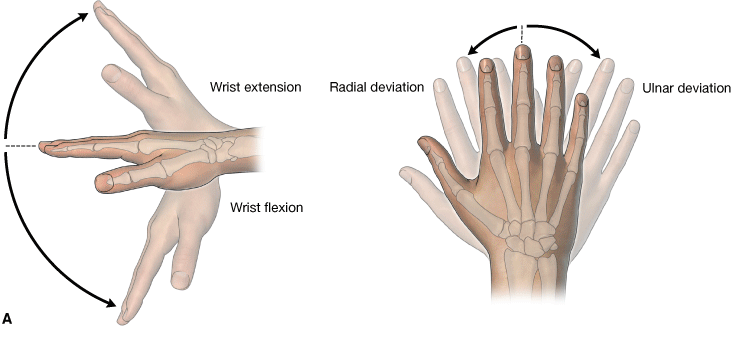
\includegraphics[width=0.5\textwidth]{figures/anatomy/flexexulradev}  %<--but is not needed.
	\caption{Flexion, extension and radial and ulnar deviation of the hand. Modified from \cite{zezo2016}}
	\label{fig:wristMove}
\end{figure}

Several more muscles in addition to those responsible for ulnar and radial deviation are involved with the flexion and extension of the wrist. Like the other muscles, the flexor and extensor muscles also extend through the whole forearm from the distal part of humerus and proximal parts of radius and ulnar to the metacarpal bones in the wrist. Many of these muscles are included in movements of both radial/ulnar deviation and flexion/extension, though flexion/extension have one muscle who is only used for flexion at the wrist, the palmaris longus muscle. This can be explained as more force is usually needed in flexion at the wrist than in extension or radial/ulnar deviation.\\
Though several of the same muscles are included in both types of movement, studies have shown that it is possible to differentiate between recorded EMG signals from these muscles when performing radial/ulnar deviation and flexion/extension at the wrist. \cite{hahne2014} In \figref{fig:ALL_THE_MUSCLES} the muscles in the forearm both involved with extension/flexion and radial/ulnar deviation is marked with boxes around the name of the muscles. 

\begin{figure}[H]
	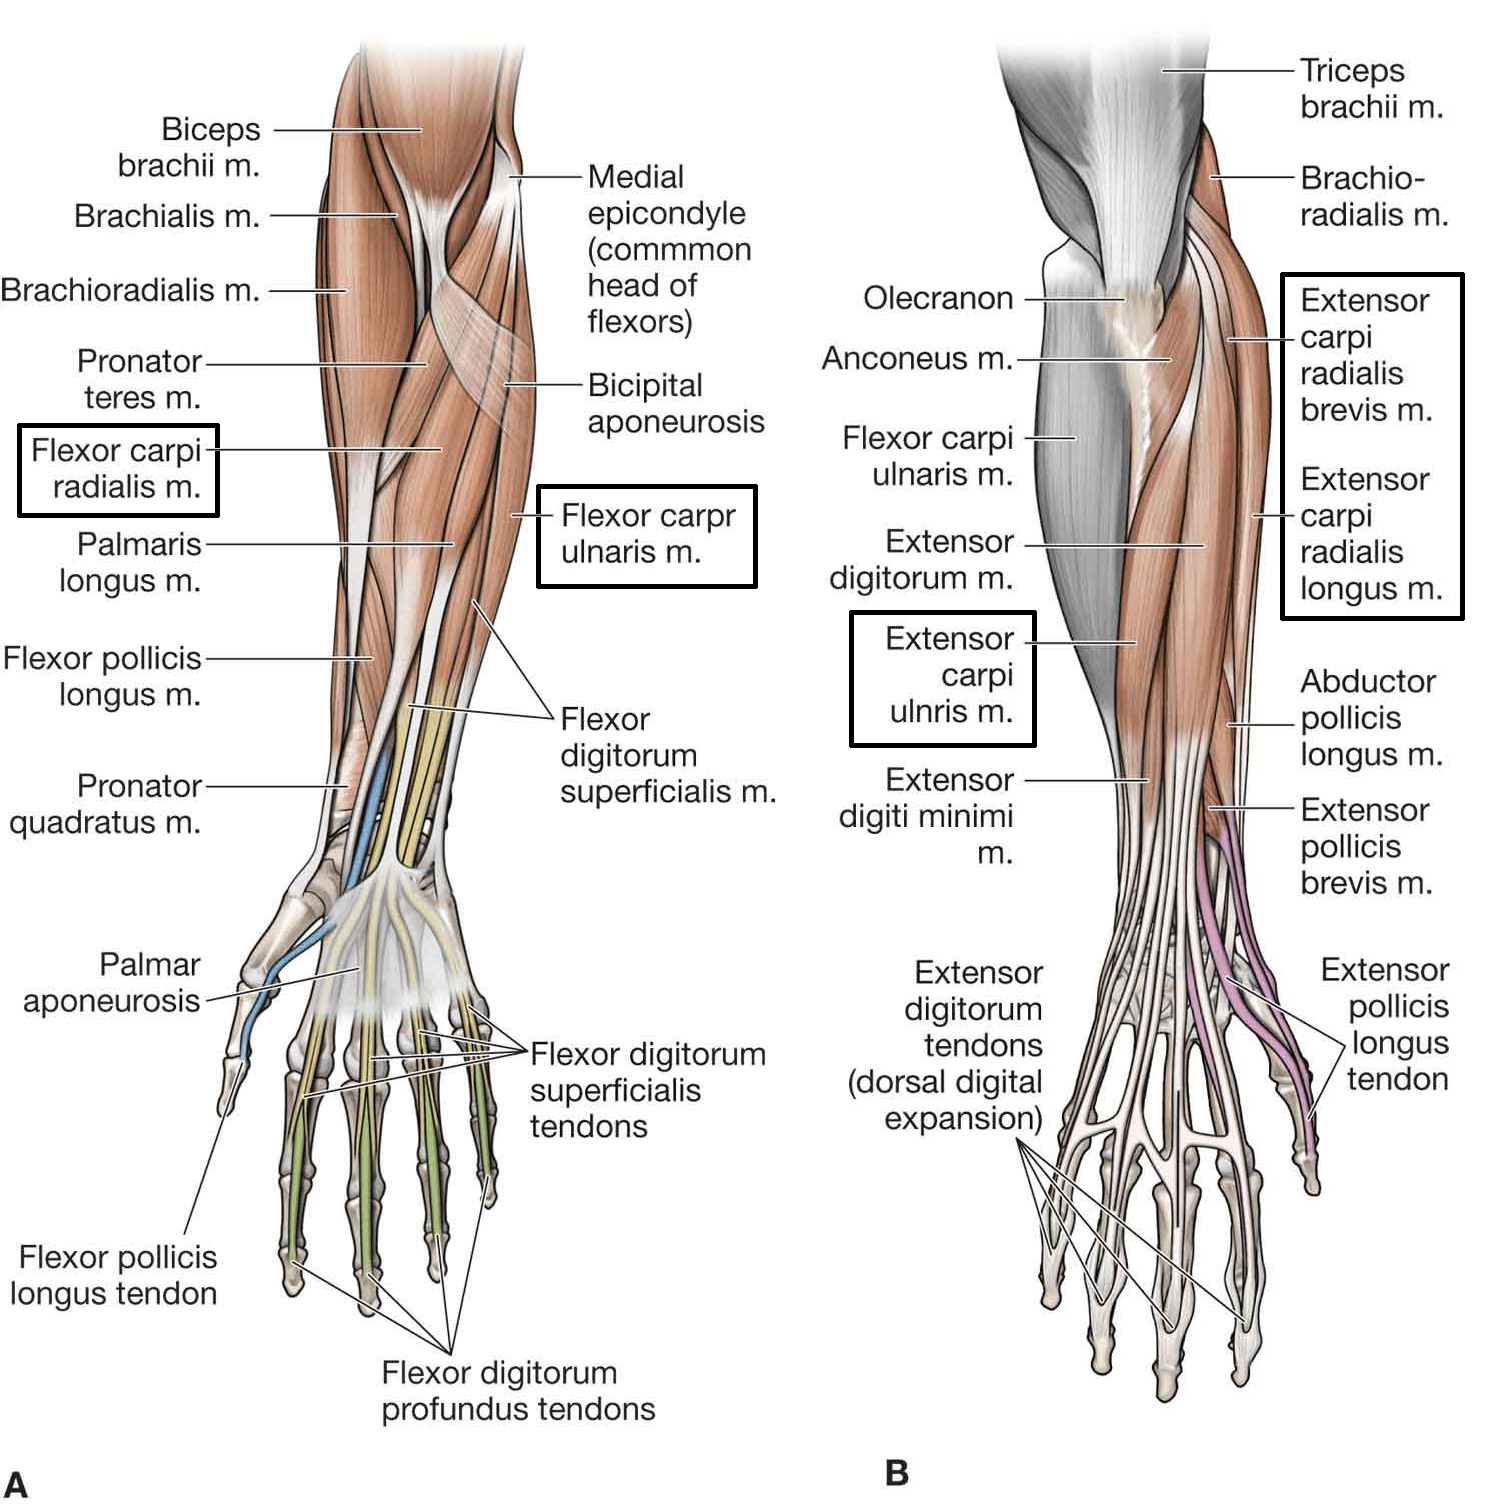
\includegraphics[width=0.7\textwidth]{figures/anatomy/all_the_muscles}  %<--but is not needed.
	\caption{\textbf{A)} anterior view of lower muscles. \textbf{B)} posterior view of lower muscles. The muscle names in the boxes are muscles which are included in both extension/flexion and ulnar/radial deviation at the wrist. Modified from \cite{zezo2016}.}
	\label{fig:ALL_THE_MUSCLES}  %<--give the figure a label, so you can reference!
\end{figure}

%Muscles involved with pronation of the wrist includes the pronator quadratus and pronator teres muscles. The pronator quadratus muscle is located near the wrist and is fixated on the distal portions of both ulna and radius, from where is forms a wide band across the gap of the two bones. The pronator teres is located near the elbow, where it originates  from the medial distal part of humerus and the medial lateral part of ulna, to reach across the anterior part of the forearm and fixate to the midlateral surface of radius. 
%There is only one muscle involved in the process of supination of the forearm, the supinator. The supinator muscle sits opposite the pronator teres muscle near the elbow, where it originates from the lateral distal part of humerus and the lateral proximal part of ulna and fixate on the anterolateral surface of radius. 
%These three are the only muscles responsible for pronation and supination of the forearm. Therein exists a problem in detecting viable EMG signals to properly detect pronation and supination gestures, since the muscles involved does not extend through the forearm as most other muscles in the forearm.

%Extension and flexion of the fingers include most of the muscles in the lower arm. Most of these muscles extend throughout the whole forearm as most of them originates from the lateral surfaces of humerus or the proximal portions of ulna and radius, and extends towards the wrist and fingers to fixate on the metacarpal bones in the wrist and through tendons fixate on the different phalanges bones of the fingers and thumb. See FIGURE \ref{fig:wrist} and \ref{fig:wristFingers} for a detailed overview of each muscles origin, insertion and action it performs. 
%
%\begin{figure}[H]
%	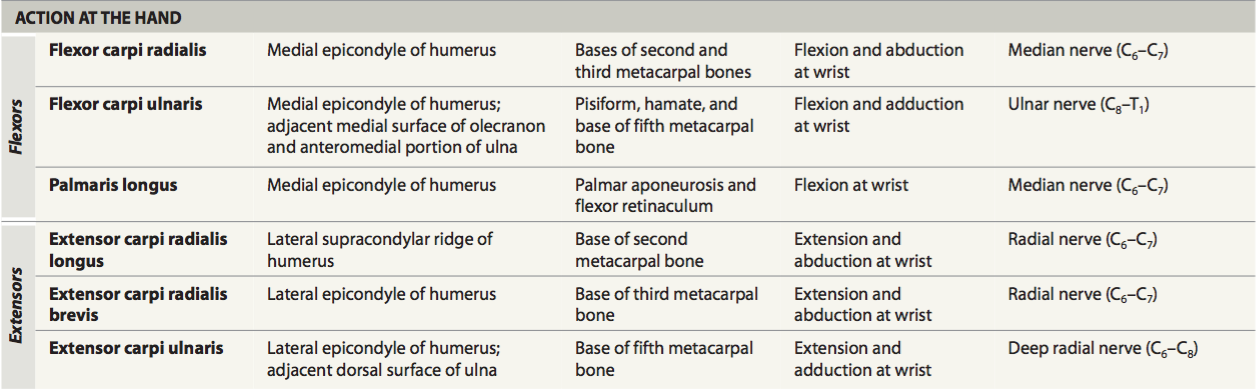
\includegraphics[width=.4\textwidth]{figures/Anatomy/wrist}  %<--but is not needed.
%	\caption{Table of the muscles in the forearm involved with movements of the wrist. \cite{martini}}
%	\label{fig:wrist}  %<--give the figure a label, so you can reference!
%\end{figure}
%
%\begin{figure}[H]                    
%	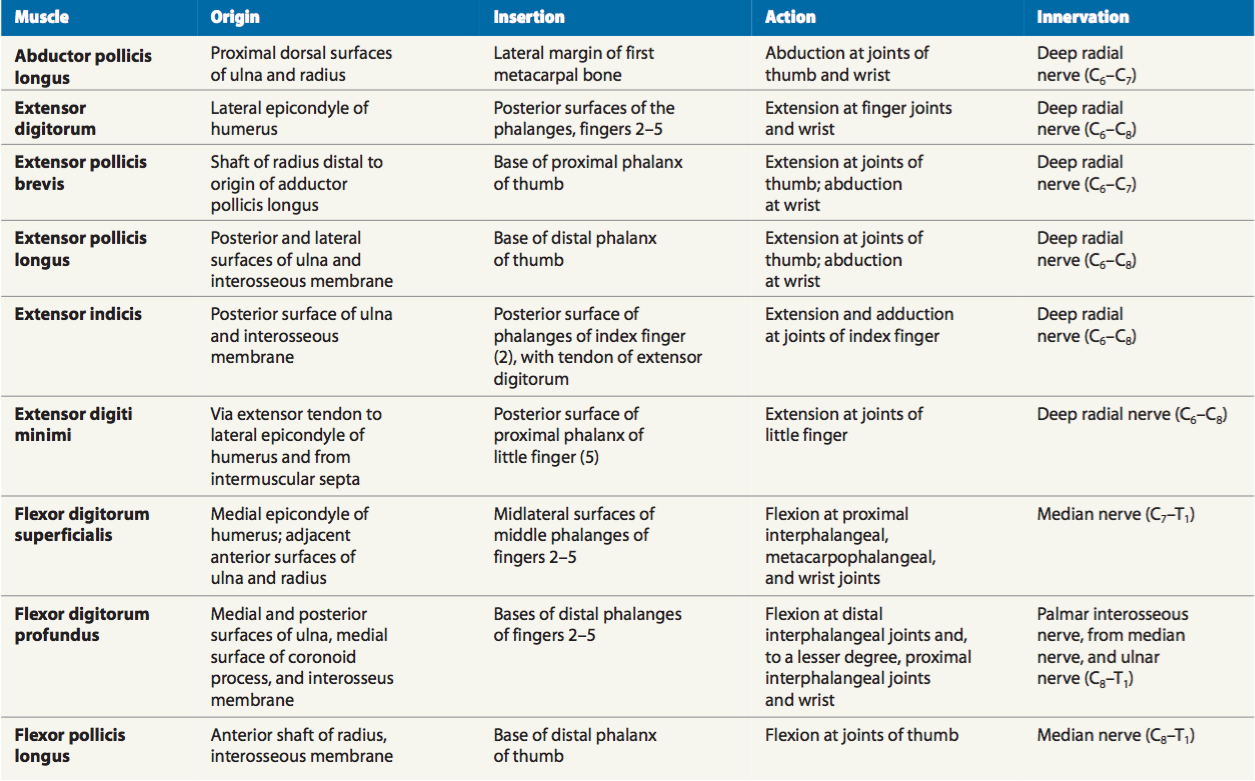
\includegraphics[width=.4\textwidth]{figures/Anatomy/wristFingers}  %<--but is not needed.
%	\caption{Tabel of muscles in the forearm involved with movements of the wrist and fingers. \cite{martini}}
%	\label{fig:wristFingers}  %<--give the figure a label, so you can reference!
%\end{figure}



%abductor pollicis longus
%extensor pollicis longus
%extensor pollicis brevis
%extensor indicis
%supinator
%anconeus
%extensor digitorum
%extensor digiti minimi
%pronator quadratus
%flexor digitorum superficialis
%brachialis
%flexor pollicis longus
%flexor digitorum profundus
%brachioradialis
%flexor carpi ulnaris
%pronator teres
%extensor carpi ulnaris
%extensor carpi radialis brevis
%extensor carpi radialis longus
%palmaris longus
%flexor carpi radialis




%tail


\section{Origin of electromyography} \label{sec:physiology}
This project will use EMG to map the hand gestures mentioned in the previous section. In this section it will be described how the EMG signal is generated.% and which problems that can occur in detecting it. 

The electric potential detected with electromyography is an action potential causing the muscle to contract. Certain mechanisms are involved for this to happen. The motor unit of the muscle needs to be activated alongside with its associated alpha motor system, which is the lower motor neuron, its axon, and the muscle fibres the motor unit innervates. The muscle fibre is an excitable cell with a resting potential of between -90mV and -70mV. A threshold of approximately -55mV needs to be reached for an action potential to be generated, this is visualised in \figref{fig:action_potential}. The sarcolemma, the membrane covering the muscle fibres, has sodium and potassium ion channels that maintains the resting potential, depolarize the muscle fibre if the threshold is exceeded or repolarize the muscle fibre. \cite{cram2012}


\begin{figure}[H]
	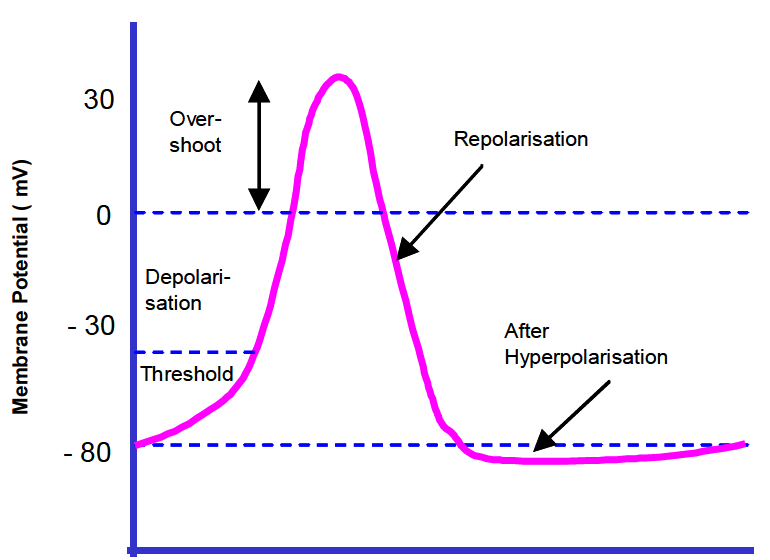
\includegraphics[width=0.5\textwidth]{figures/Anatomy/action_potential}  %<--but is not needed.
	\caption{Illustration of the action potential exceeding the threshold for it to be generated and the following depolarization and repolarization. \cite{konrad2005}}
	\label{fig:action_potential}  %<--give the figure a label, so you can reference!
\end{figure}

The lower motor axon is branching out so that it can attach to the muscle fibre at the motor end-plate and create neuromuscular synapses. The action potential traveling down the axon reaches the synapses and releases Acetylcholine (ACh). ACh raises the permeability of the cell membrane where sodium ions influx and causes the membrane to depolarize. Calcium ions are released and binds with troponin and expose the active sites on the thin filaments which allows the muscle to contract. The action potential travels along the whole muscle fibre through t-tubuluses, as depicted in \figref{fig:EMG_generation}. This happens in both directions from the motor end-plate to the tendinous attachment. When the peak of the depolarization of about 30mV is reached a rapid efflux of potassium ions causes the muscle fibre to repolarize and reach its resting potential again. \cite{cram2012}

\begin{figure}[H]
	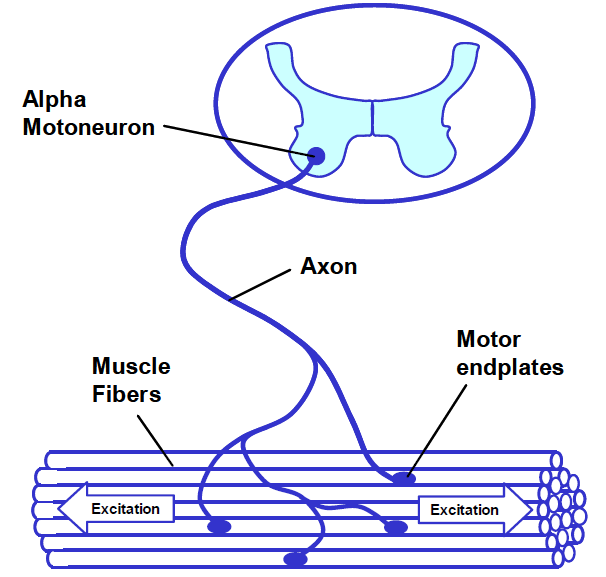
\includegraphics[width=0.4\textwidth]{figures/Anatomy/EMG_generation}  %<--but is not needed.
	\caption{Illustration of the action potential exciting the muscle fibre, which causes the release of calcium ions and the muscle to contract. \cite{konrad2005}}
	\label{fig:EMG_generation}  %<--give the figure a label, so you can reference!
\end{figure}

Depending on the force that needs to be applied for a given task more or less motor units are activated and therefore more or less muscle fibres are contracted. The bigger the force the more motor units are activated. Furthermore, the number of muscle fibres per motor unit varies between muscles in the human anatomy. The finer the movement the higher the innervation, e.g. the lower arm muscles have a higher innervation than those in the quadriceps. \cite{cram2012}

\subsection{EMG states}
Motor unit action potential (MUAP) can be easily decribed as the addition of the action potentials emerging from the muscle fibers comprising the motor unit. The EMG signal is the result of the inclusion of different MUAP.

 %JACOB COMENT:and can be divided into two main states, the transient state and the steady state.Before write is true for  ramp and hold contraction not for every contraction (training protocol related)
 The transient state is related to the beginning phase of the muscle contraction, while the steady state is the stable phase of the muscle contraction when a constant position is held. \cite{mobarak2014}

Although the steady state only contains a short temporal structure of the patterns involved in the contraction of the muscle \cite{mobarak}, studies has shown that it is possible to achieve online continuous control using steady-state EMG signals. A study by Englehart et al. \cite{} demonstrated that steady-state data classified more precisely than transient state data. This could be due to the fact that a larger amount of meaningful data is contained in this muscle contraction phase \cite{mobarak} For the training of the control system  in this project the steady signal will then be used. %However there are still limitations due the fact that the classifier can not deal with the transient EMG signals. Some clinical applications that combine both data have shown an increase in the recognition system.  

%the extraocular muscle has the highest innervation of 3:1 and the gastrocnemius muscles has one of 2000:1. \cite{cram2012}

%(Something about how the innervation is in certain muscles of the forearm. Also argue that humans can perform more dexterous movement when the ratio of muscle fibers to motor units is low) (maybe around 100:1)

%(something about how the EMG signal is affected when the limb is positioned differently)
% following section move to the "conclusion of the background" section
%As mentioned this project focuses on the mapping of different hand gestures. This mapping relies on that the generated EMG from the different hand gestures are differentiable. For a prosthetic user a good performing prosthesis must perform hand gestures as well in an elevated limb position as in a seated position to be able to support the user in daily tasks, e. g. taking a cup from a cupboard and pouring water into the cup. However, changes in the EMG occurs when performing the same hand gestures in different limb positions. These signal alternations can occur for different reasons. Changing the limb position can lengthen the muscles and result in a change in the signal source relative to the electrode from which the EMG signal is obtained, and even the lengthening of the muscles itself due to changing limb position will alter the EMG activity caused by a degree of overlap of the thick and thin filaments. Other findings has shown that the activity of certain muscles' is depending on angles of joints besides those primarily actuating the contraction of these muscles. \cite{Fougner2011} Thus, this limb position effect must be seen as an important aspect to take into consideration in the mapping of hand gestures to control a prosthesis for the user to receive a good performing support device. 
\section{Instrumentation} \label{sec:myoband}
	% former Myo armband -section
%What does the band consist of?
%Electrodes, gyroscope and accelerometer
%Build-in filters and stuff like that?
%Sampling frequency

%head
The following section will contain a presentation of the Myo armband from Thalmic Labs, which will be used for data acquisition in this study and an explanation of acquiring EMG signals using surface electrodes.

\subsection{Myo armband}

The Myo armband is a device developed by Thalmic Labs capable of identifying hand gestures and arm movements in order to interact and control different electronic devices. The system can be used with software provided by Thalmic Labs to control a limited range of devices using the data from the armband.
%However, standard use of the system does not provide use of the raw data, which is necessary for this project. The system does however allow data to be extracted from the armband, with without involving the software from Thalmic Labs. This enables to acquire data to process in Matlab. 
The Myo armband is illustrated in \figref{fig:armband}. 

\begin{figure}[H]                    
	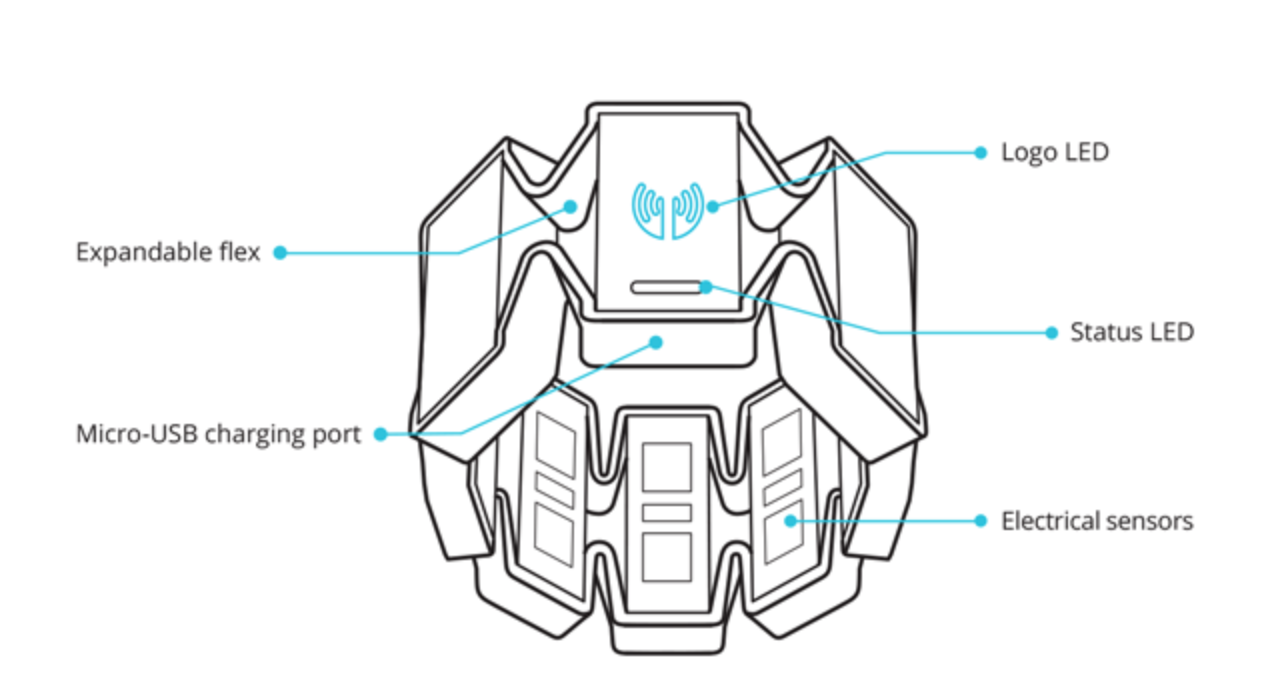
\includegraphics[width=.5\textwidth]{figures/myob/armband}  %<--but is not needed.
	\caption{Main components of the Myo armband. \textbf{SOURCE}}
	\label{fig:armband}  %<--give the figure a label, so you can reference!
\end{figure}


%The main components of the Myo armband illustrated in the figure \ref{fig:armband} are:
%\begin{itemize}
%\item The logo LED gives information about the sync state. The LED is solid when you perform the Sync Gesture successfully and
%the Myo armband is synced to your arm. The LED pulses when the armband is not synced.
%\item The status LED shows the state of the Myo armband. When it lights up in blue once the Myo armband is connected to a device. 
%\item The USB charging port allows to charge the Myo armband battery. 
%\end{itemize}
%The systems counts with sizing clips, these small pieces give a tighter grip which is more appropriated for smaller arms.

The Myo armband has eight medical grade stainless steel surface EMG sensors. %responsible of recognizing each gesture. 
These electrodes are dry and therefore not covered in silver chloride gel to reduce impedance between the electrode and skin. However, it has been shown by Mendez et al. \cite{Mendez2017} that the EMG recorded with the Myo armband is a suitable acquisition system for mapping hand gestures compared to conventional EMG acquisition. The only mapping method used in that study was linear discriminant analysis, and it is noted that other mapping methods should be investigated to further validate the quality of mapping the EMG obtained by the Myo armband. The Myo armband is sampling sEMG data at a sample rate of 200 Hz. A low sample rate could result in problems of aliasing later on in the data processing, since the range of the sEMG signal is 10-500 Hz. \cite{cram2012} 

In addition, it has a nine axis inertial measurement unit (IMU) which enable the detection of arm movement. An IMU is an electronic device that provides information concerning position and orientation for navigation and stabilization purposes. The IMU's in the Myo armband comprises a three axis accelerometer, a three axis gyroscope and a three axis magnetometer. The accelerometer measures the physical acceleration experienced by an object, where the object in this case is the body part where the Myo armband is placed. 
%It gives information about the acceleration experienced relative to free fall and expresses this in g-force. One g-force being when the accelerometer is at rest on the Earth's surface. That is since all points on the surface of the Earth is accelerating upwards relative to an object in free fall near the surface. For the g-force to change from one g-force the accelerometer must be exposed to motion. 
The gyroscope has the property of measuring angluar velocity. The magnetometer has the property of a compass, measuring the earth's magnetic field. This enables the armband to provide data on orientation. IMU data is sampled at a sample rate of 50 Hz. The Myo armband communicates through Bluetooth 4.0 to a computer.
%(something about the actual data the myoband provides and how many axes a magnometer actually has). \textbf{SOURCE}
%\textbf{more text on the data types we are going to get from the IMU's} 
% ... (It is equipped with an ARM Cortex-M4 microprocessor of low energy consumption.)

%\begin{figure}[H]                    
%	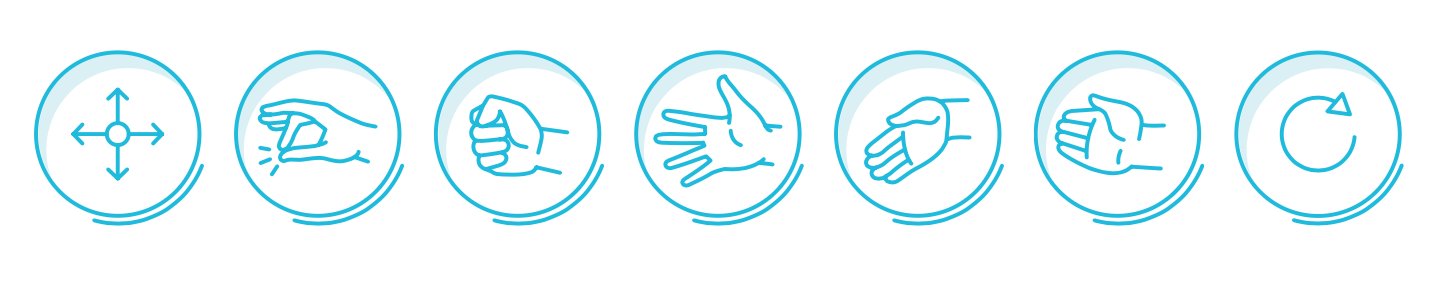
\includegraphics[width=.5\textwidth]{figures/myob/gestures}  %<--but is not needed.
%	\caption{Hand gestures and movements detected by the Myo armband using its own interface from Thalmic Labs. SOURCE}
%	\label{fig:gestures}  %<--give the figure a label, so you can reference!
%\end{figure}
%It offers five pre-defined gestures as showed in the figure \ref{fig:gestures}, it provides haptic feedback through short, medium or long vibrations to correct moves or activate the system.

%JACOVB COMENT:sample rate high enough


%This means that many high-frequencies of the sEMG signal will not be recorded, and aliasing could have an influence on the recorded signals due to not respecting the Nyquist Law of sample rate. 
%Thus, the Myo band arm supplies two kinds of data, the IMU data and EMG data. %which is spatial and gestural. 
%The IMU data add information about the orientation and movement of the user's arm. This information is provided through the accelerometer and the gyroscope. EMG recordings gives information about the users hand gestures. The recorded signals can be send to other devices using Bluetooth 4.0.


%/begin{figure}
%poner imagen del los gestos%
%/end{figure}

%How does it communicate with the computer?
%Connection
%Programs that can be used to interface with the arm
%What kind of data will be received from the myo band?


%it connecrs to a PC or tablet via bluetooth Low Energy and allows both raw data streaming and the use of a proprietary library for gesture recognition.The signal processing is performed on the host platform and the used algorithms are not documented (poner de otra manera)



%\section{JACO2 robotic arm}

In this section a briefly description of the JACO$^2$ robotic arm will be given. It is a 6 DOF robotic arm  with a three fingered hand developed by Kinova Robotics. It is lightweight $\left( 4.4 kg\right)$, which makes this machine specially usable in assistive and collaborative applications. It is designed to help people with upper body disabilities in order to gain more autonomy in ordinary daily tasks.\\

\begin{figure}[H]                    
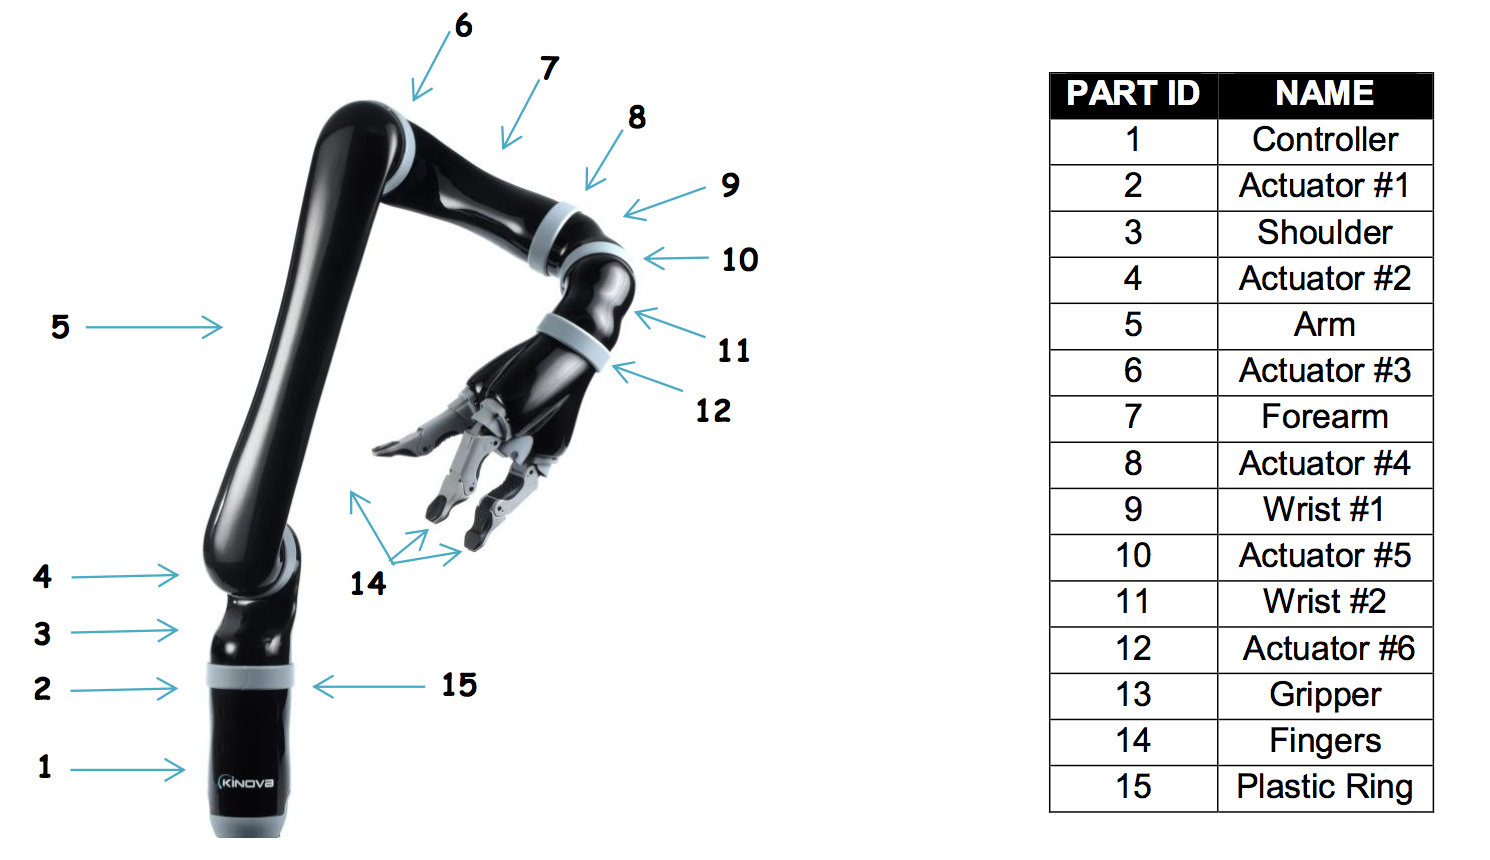
\includegraphics[width=.3\textwidth]{figures/Jaco/roboticarm}  %<--but is not needed.
\caption{6 DOF JACO$^2$ robotic arm from Kinova Robotics. \cite{kinova2017}}
\label{fig:roboticarm}  %<--give the figure a label, so you can reference!
\end{figure}
\textbf{new more exciting picture of the same thing}

The JACO$^2$ is a serial manipulator, which means that this kind of robotic arm is designed as a series of links connected by motor-actuated joints that extend from a base to an end-effector. Any movement in a joint affects all the following joints and links in the chain. The arm can by default be controlled with the help of a joystick, but it can be programmed in C++ to be controlled by other means, using the software development kit (SDK) provided by the manufacturer.\\

\textbf{include picture of JACO arm with all the names of things on/in it.}

%The control of the JACO$^2$ arm can be Angular and Cartesian. In Angular control each actuator moves separately. Cartesian robots called Gantry robots as well, are mechatronic devices which make linear movements in three axes, perpendicularly oriented to each other. It allows eight movements:
%\begin{itemize}
%\item Three translations
%\item Three rotations of the wrist
%\item Two movements of the fingers $\left( open/close\right) $
%\end{itemize}


\section{Preprocessing of EMG}

%HEAD
Before recorded EMG signals can be utilized in control of prosthetics, the signals must be processed. This section will provide information on preprocessing of the signal with filtering and noise reduction, following with feature extraction.

As mentioned in \secref{sec:myoband} sEMG is in a 10-500 Hz range. Thus it is recommended to implement a bandpass filter from $10$ to $500$ Hz in order to avoid low frequency movement artifacts in the recorded signal. 
%If the EMG is acquired from an area close to the heart, it would be preferable to filter from $100$ Hz in order to avoid recording artifacts from the heart. 
A downside to this bandwidth is that fatigued muscles will fire at a lower rate, which means the performance of the system will be affected when the subject gets tired. \cite{cram2012} %Due to the frequency spectrum of the Myo band, it isn't required to implement a bandpass filter. Instead the signal will be subjected to a highpass filter from $5$ Hz. (The frequency spectrum should be mentioned in the Myo band section and not here I think)

In order to achieve a higher signal to noise ratio (SNR) it is common practice to perform preprocessing of the signal%, including input impedance, differential amplification and filtering. 
The raw EMG signals has to be preprocessed due to them being sensible to noise elements from the surroundings, since the range of the signal is in the order of millivolts to microvolts. To acquire a high SNR, the input impedance of the amplifier has to be between $10$ and $100$ times the impedance at the skin-electrode interface \cite{cram2012}.

%Input impedance is determined by a simple rule in order to avoid defeating the common mode rejection of the EMG amplifier. The rule states that the input impedance of the EMG amplifier has to be between $10$ and $100$ times higher than the impedance of the skin-electrode interface. \cite{cram2012}

Differential amplification is used in EMG in order to amplify the original signal and remove common signals from two or more electrodes, in order to avoid common noise from more electrodes in the amplified signal. The amplifier must have a built in gain as well which determines the final strength of the signal, and both of these features are implemented in order to maximize the SNR. 
%Basic filtering should be implemented in order to avoid electrical noise. 
%This filter would be implemented as a notch filter, in order to reject the electrical noise and achieve a higher SNR. 
%The low-pass filtering will ensure avoiding aliasing in the signal, because is will filter out frequencies higher than the used samplings frequency. The high-pass filter will filter out movement artifact, and thus stabilizing the baseline. \cite{cram2012}

%This is done in order to make sure the final signal does not contain irrelevant high and low frequencies.\cite{cram2012}

%feature extraction follows here as a sbusection
\subsection{Feature extraction}

% Use 'Linear and non linear regression techniques for Simultaneus and prop...' + 'Feature reduction and selection for EMG signal classification'

%HEAD
%The following section will feature feature extracion, 

Following preprocessing of the recorded EMG signal, features can be extracted and used to map different hand gestures. Features are extracted from the signal to represent the signal using fewer data samples. This is also called dimension reduction and result in faster computation times. When analyzing EMG signals there will be three different signal components to be extracted, which are the frequency and time domains, as well as the time-scale representation. Frequency domain features require a Fourier transformation of the signal, which requires more processing than the direct extraction of time domain features. \cite{phiny2012}
%In order to extract the features which can be used to differ between the movements performed by the wearer, different features can  extraction can be implemented. In addition to highlighting important features within the signal, the implementation of feature extraction will be useful when it comes to removing unwanted signal features caused by noise sources such as the powergrid and movement of the electrodes. \cite{phiny2012}

The time domain features are extracted directly from the EMG signal, and these feature extraction methods are often used both for research and practices since they often require very little processing compared to frequency domain features. Time domain features are mainly focused on the amplitude of the signal, which means they have a disadvantage if the signal differs in amplitude due to muscle fatigue. \cite{phiny2012} Different features are visualized in \figref{fig:EMGfeatures}. 

\begin{figure}[H]                    
	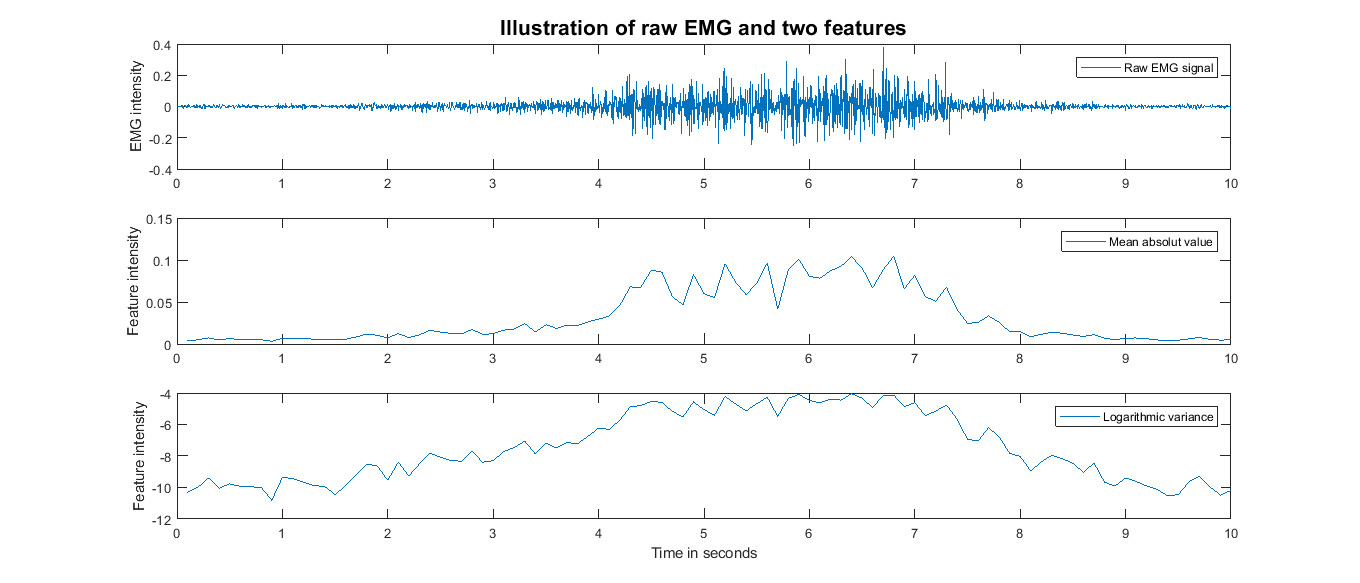
\includegraphics[width=.5\textwidth]{figures/background/EMG_features}  %<--but is not needed.
	\caption{Above a raw EMG signal. Below are different features extracted from the EMG signal presented.}
	\label{fig:EMGfeatures}
\end{figure}

%Based on the study af Hahne et al. \cite{hahne2014}, we will choose logarithmic variance as the feature to be extracted from the recorded EMG signal. Hahne et al. finds that the cross-validation performance improves significantly with the use of linear regression combined with logarithmic variance, compared to combining the linear regression with variance or RMS. \cite{hahne2014}. 

%Choice of feature will be based on previous studies of performance of different extracted features. 
%%, where the method will be chosen based on it's performance in the low frequency area and the processing time for the feature to be extracted. 
%This is a result of the Myo armband limiting the recordable signal to 100 Hz, and the intend of being able to control the JACO arm in real-time, where a long processing time would cause a delay between hand movement and movement of the JACO arm.
%This study will only implement time domain features, due to the low sampling rate of the Myo band, which means that an implementation of frequency domain features will not be useful, as the signal does not contain a lot of information in that domain. The feature chosen in this study will be the logarithmic variance of the signal, based on a previous study by \cite{hahne2014}, where they find that this feature is useful for methods based on the numerical range of the features. \cite{hahne2014} 
\section{Regression methods}

%Linear regression:
	%linear regression (how well the line fits the data can be decided with goodnes of fit or least squares)
	%multiple linear regression
	%principal components regression
	%bayesian linear regression
%non-linear regression:
	%kernel ridge regression
	%gaussian regression 
	

%head
Regression methods are widely used is statistics as a method to determine relationship between variables. It can be used to extract relations to predict future developments or tendencies in a given data set. It is also a commonly used method to evaluate EMG signals to determine different parameters. 
%There exist many regression methods, but overall to classes of methods can be defined; linear and non-linear, some of which will be covered in this section. 

The most basic form of regression is linear regression, which is a test for linear dependency between two variables. In simple linear regression it is investigated how one, dependent variable, is related to another, independent variable. The term \textit{simple} denotes that only two variables are being considered simultaneously. The equation for simple linear regression is: \cite{zar2009}
\begin{equation}
Y_i = \alpha + \beta X_i
\end{equation}

Performing simple linear regression finds the correlation between the tested variables, and is expressed by the correlation coefficient. This coefficient describes how the two variables relate to each other by how the development of one variable is dependent on the the other. Thus a positive correlation represent that a change in one variable will resolve in a similar change in the other variable as well. On the contrary, a negative correlation imply that change in one variable will resolve in an opposite change in the other variable. If no correlation is present between the two variables no change in either variable will resolve in change in the other, and it can therefore be determined that the two variables has no relation to each other. \cite{zar2009}
The simple correlation coefficient is calculated as: \cite{zar2009}
\begin{equation}
r = \frac{\sum xy}{\sqrt{\sum x^{2} \sum y^{2}}}
\end{equation}

Furthermore a coefficient of determination can be calculated to express how much of the variability of the dependent variable is accounted for when regressing upon the independent variable. This coefficient is denoted $r^{2}$ and can be calculated by simply squaring the correlation coefficient ($r$). 
Both $r$ and $r^{2}$ can be used to determine the strength of the relationship between the two tested variables. \cite{zar2009}


%fit of a straight line to best fit several data points. This regression method is widely used in studies where it is used to describe a simple relationship between a dependent and independent factor.

A variant of the linear regression is the multiple linear regression, which can be used in cases where the relationship between three or more variables is wished to be investigated. Here it is considered that one of the variables are dependent on two or more independent variables. 
Multiple linear regression can be used in cases where two or more variables are expected to have a linear correlation to a dependent variable and it is wished to find which of the independent variables who has the biggest influence on the dependent variable, so to say the highest correlation coefficient. 
Since multiple linear regression is based upon simple linear regression, it is modelled after the equation for simple linear regression. However, as $Y$ can be dependent on more than one other variable at times, another can be added to the equation: \cite{zar2009}
\begin{equation}
Y_i = \alpha + \beta_1 X_1i + \beta_2 X_2i + \epsilon_i \ \ \ \ ,
\end{equation}
, where the sum of the error ($\epsilon$) is zero and is assumed to be normally distributed.

When three variables are present in the equation, the visual representation of the regression is in the 3rd dimension, and will no longer be presented as a line in 2D, but as a plane in 3D. Having more than three variables will resolve in a regression in the $m$-dimension, where $m$ is the number of variables. This plane of regression is called the hyperplane. However, regression is not a perfect fit to every sample point, and thus the equation for three or more variables is only complete when the error is also calculated, denotes as $\epsilon$.

There exist ofcourse cases where the relationship between more than three variables is wished to be investigated. In such cases, each new variable can be added to the equation, and the final can be expressed in a summed up equation: \cite{zar2009}
\begin{equation}
Y_j = \alpha + \sum_{i=1}^{m} \beta_j X_ij + \epsilon_j \ \ \ \ ,
\end{equation}
where $m$ is the number of variables.

There exist no limit to the number of variables which can be tested, however there should always be at least two observations more than the number of variables, so that $n \geq m+2$. Otherwise multiple linear regression is not possible. \cite{zar2009}




%one dependent variable and several independent are to be described and a generalization of the relationship between the variables wish to be found. 

%Principal component regression is based on the principal component analysis, where a very large dataset can be compressed into a few of the most important components to further be analyzed upon. This means that in a dataset of many samples, the ones which are the most responsible or most correlated in a meaningful relationship between the dependent and independent variables, can be isolated to best describe which factors have a result on the relationship.







%tail

\section{Ik-State-of-the-Art}

%This project will focus on the mapping of different hand gestures while having the arm in different positions. This mapping relies on that the generated EMG from the different hand gestures are differentiable. 
For a prosthetic user a good performing prosthesis must perform hand gestures as well in an elevated limb position as in a seated position to be able to support the user in daily tasks, e.g. taking a cup from a cupboard and pouring water into the cup. However, changes in the EMG occurs when performing the same hand gestures in different limb positions \cite{Fougner2011, avella2006}. These signal alternations can occur for different reasons. Changing limb position can make muscles move under the skin, relative to the placement of the EMG electrodes, resolving in change of the signal source. Muscle contractions in them selves can also make changes to the recorded EMG due to change in the microscopic structure of the muscles caused by overlap of thick and thin filaments. \cite{martini}  
%can lengthen the muscles and result in a change in the signal source relative to the electrode from which the EMG signal is obtained, and even the lengthening of the muscles itself due to changing limb position will alter the EMG activity caused by a degree of overlap of the thick and thin filaments. 
Other findings have shown that the activity of certain muscles' is depending on angles of joints besides those primarily actuating the contraction of these muscles. \cite{Fougner2011} Thus, the effect of limb position must be seen as an important aspect to take into consideration in the mapping of hand gestures to control a prosthesis for the user to receive a good performing support device. %Several studies have investigated this effect. 
In 2010, Scheme et al. investigated the effect of different limb positions on pattern recognition based control. They tested eight different limb positions and processed the data using time-domain feature extraction and linear discriminant analysis. Here they found that for each limb position the classification using both EMG and accelerometer data, clearly outperformed using only EMG data. Thus, it might be insufficient to only train the control scheme in one position and expect it to translate to multiple positions. \cite{Fougner2010} 
Several studies have tried to address the problem of limb position and changes in classification accuracy in EMG controlled prosthetics, using pattern recognition. %different approaches. Patterns recognition has been used in many studies with success in classifying different movements with different limb positions. 

Fougner et al. combined EMG recordings and accelerometer data when classifying movements in five different arm positions during eight different hand gestures. Using pattern recognition they found a reduction in classification error from 18\% to 5\% when using both EMG and accelerometer data. \cite{Fougner2011} Jiang et al. used EMG data and recordings of 3D markers places on able-bodied and amputated subjects' arms when performing different hand movements in three different arm positions. They found a decrease in classification error when using training data across different arm positions. They also concluded that the limb position does have a significant effect on the estimation performance for both subject groups, but that results cannot be translated between able-bodied and amputees. \cite{Jiang2013} Krasoulis et al. used linear discriminant analysis to analyse recordings from 22 subjects (20 able-bodied, 2 amputees) performing 40 different movements at the wrist, hand and fingers. The recordings included EMG data along with accelerometer, gyroscope and magnetometer data. They found a significant increase in classification accuracy by 22.6\% when using both EMG and IMU data. \cite{Krasoulis2017} 

Based on previous studies it can be determined that a combination of EMG and IMU's can be used to achieve higher classification accuracy when classifying different hand movements in different limb positions. Thus, this project will focus on the mapping of different hand gestures while having the arm in different positions. As a novel approach this project will also investigate the possibility of using regression methods instead of recognitions methods.  



%short reviews of the papers that use patterns classification methods 


%review papers which have wokred with the problem of detecting different EMG signals with that arm in different positions. 
%also point out that the problem is known and have been addressed in several studies. 
	% use IMU: (imtiaz2014), roy2010, fougner2011, Jiang2013, Krasoulis2017, Blana2016, 
  	% propose use of IMU: jiang2012, fougner2010, 
  	
  	
  	
  	

\chapter{Methods}

\section{Training data acquistion protocol}

The inclusion criteria for the subjects is that they must be healthy and able-bodied. The subjects will perform four different hand gestures: ulnar deviation, radial deviation, flexion and extension of the wrist, as shown in \figref{fig:handgest}. The order of the execution of the movements will be the same for each subject.

\begin{figure}[H]
	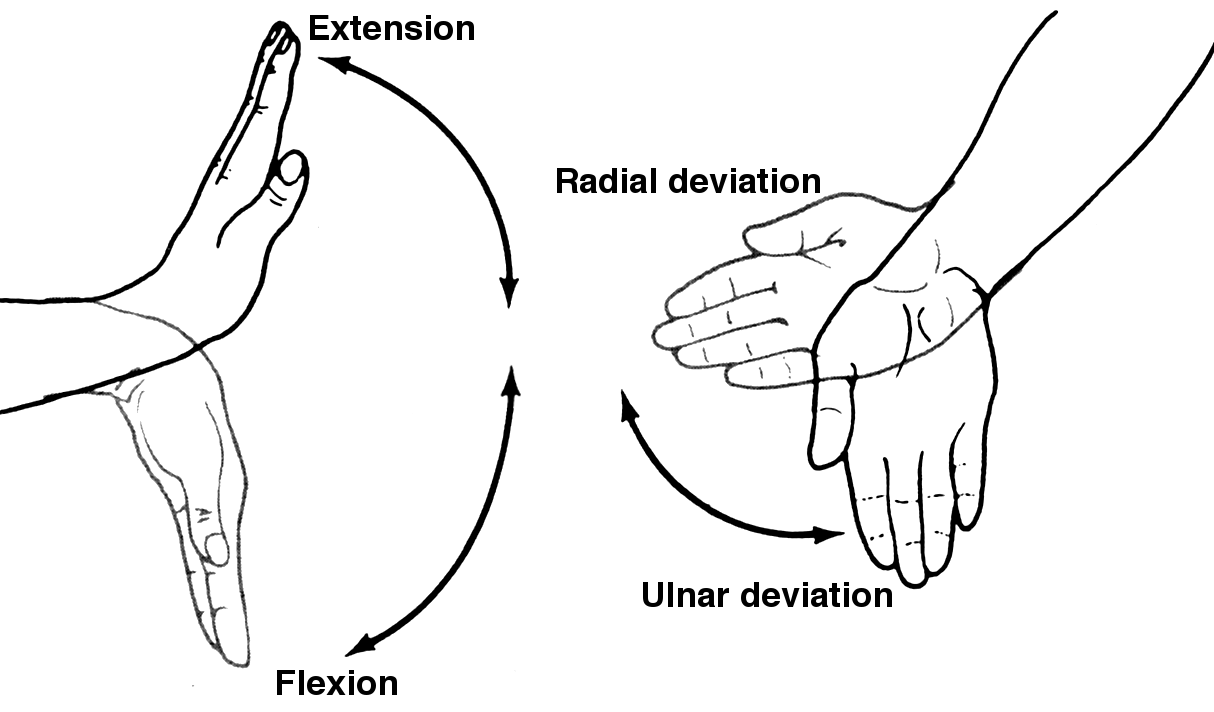
\includegraphics[width=.5\textwidth]{figures/Anatomy/wrist_move}  %<--but is not needed.
	\caption{Flexion, extension, radial and ulnar deviation of the hand. Modified from  \cite{hamilton2008}}
	\label{fig:handgest}  %<--give the figure a label, so you can reference!
\end{figure}

%In order to accomplish the study a Graphical User Interface $\left( GUI\right)$ had been created.The subjects of this study were familiar with the operation of the GUI.
At first the subject will have the baseline measured. The subject will have a relaxed forearm and hold the wrist in a neutral position. Afterwards each hand gesture will be performed as a fraction of the maximum voluntary contraction $\left( MVC\right)$ set as 30\% , 50\% and 80\%. The subjects will therefore initially be performing a MVC measure to be used as a reference measurement before the fraction of the MVC measures can be performed. The subjects will rest two minutes after the MVC measurement to avoid fatigue. This is done for each hand gesture. 

The acquisition of the fraction of the MVC of each hand gesture will consist of four chronological phases: a relaxed phase, a transition phase, a plateau phase and a relaxed phase, which will be depicted as a trapeze in a plot. The EMG of the subject will be depicted as a small circle in the plot, and the subject must follow the shape of the trapeze with the circle as best as possible. The recording of one fraction of MVC of one hand gesture will take ten seconds, where the phase with the highest contraction is four seconds. 
This procedure will be performed in three different limb positions, illustrated in the figure \figref{fig:limbpos}.

%maybe change the limb positions
\begin{figure}[H]                    
	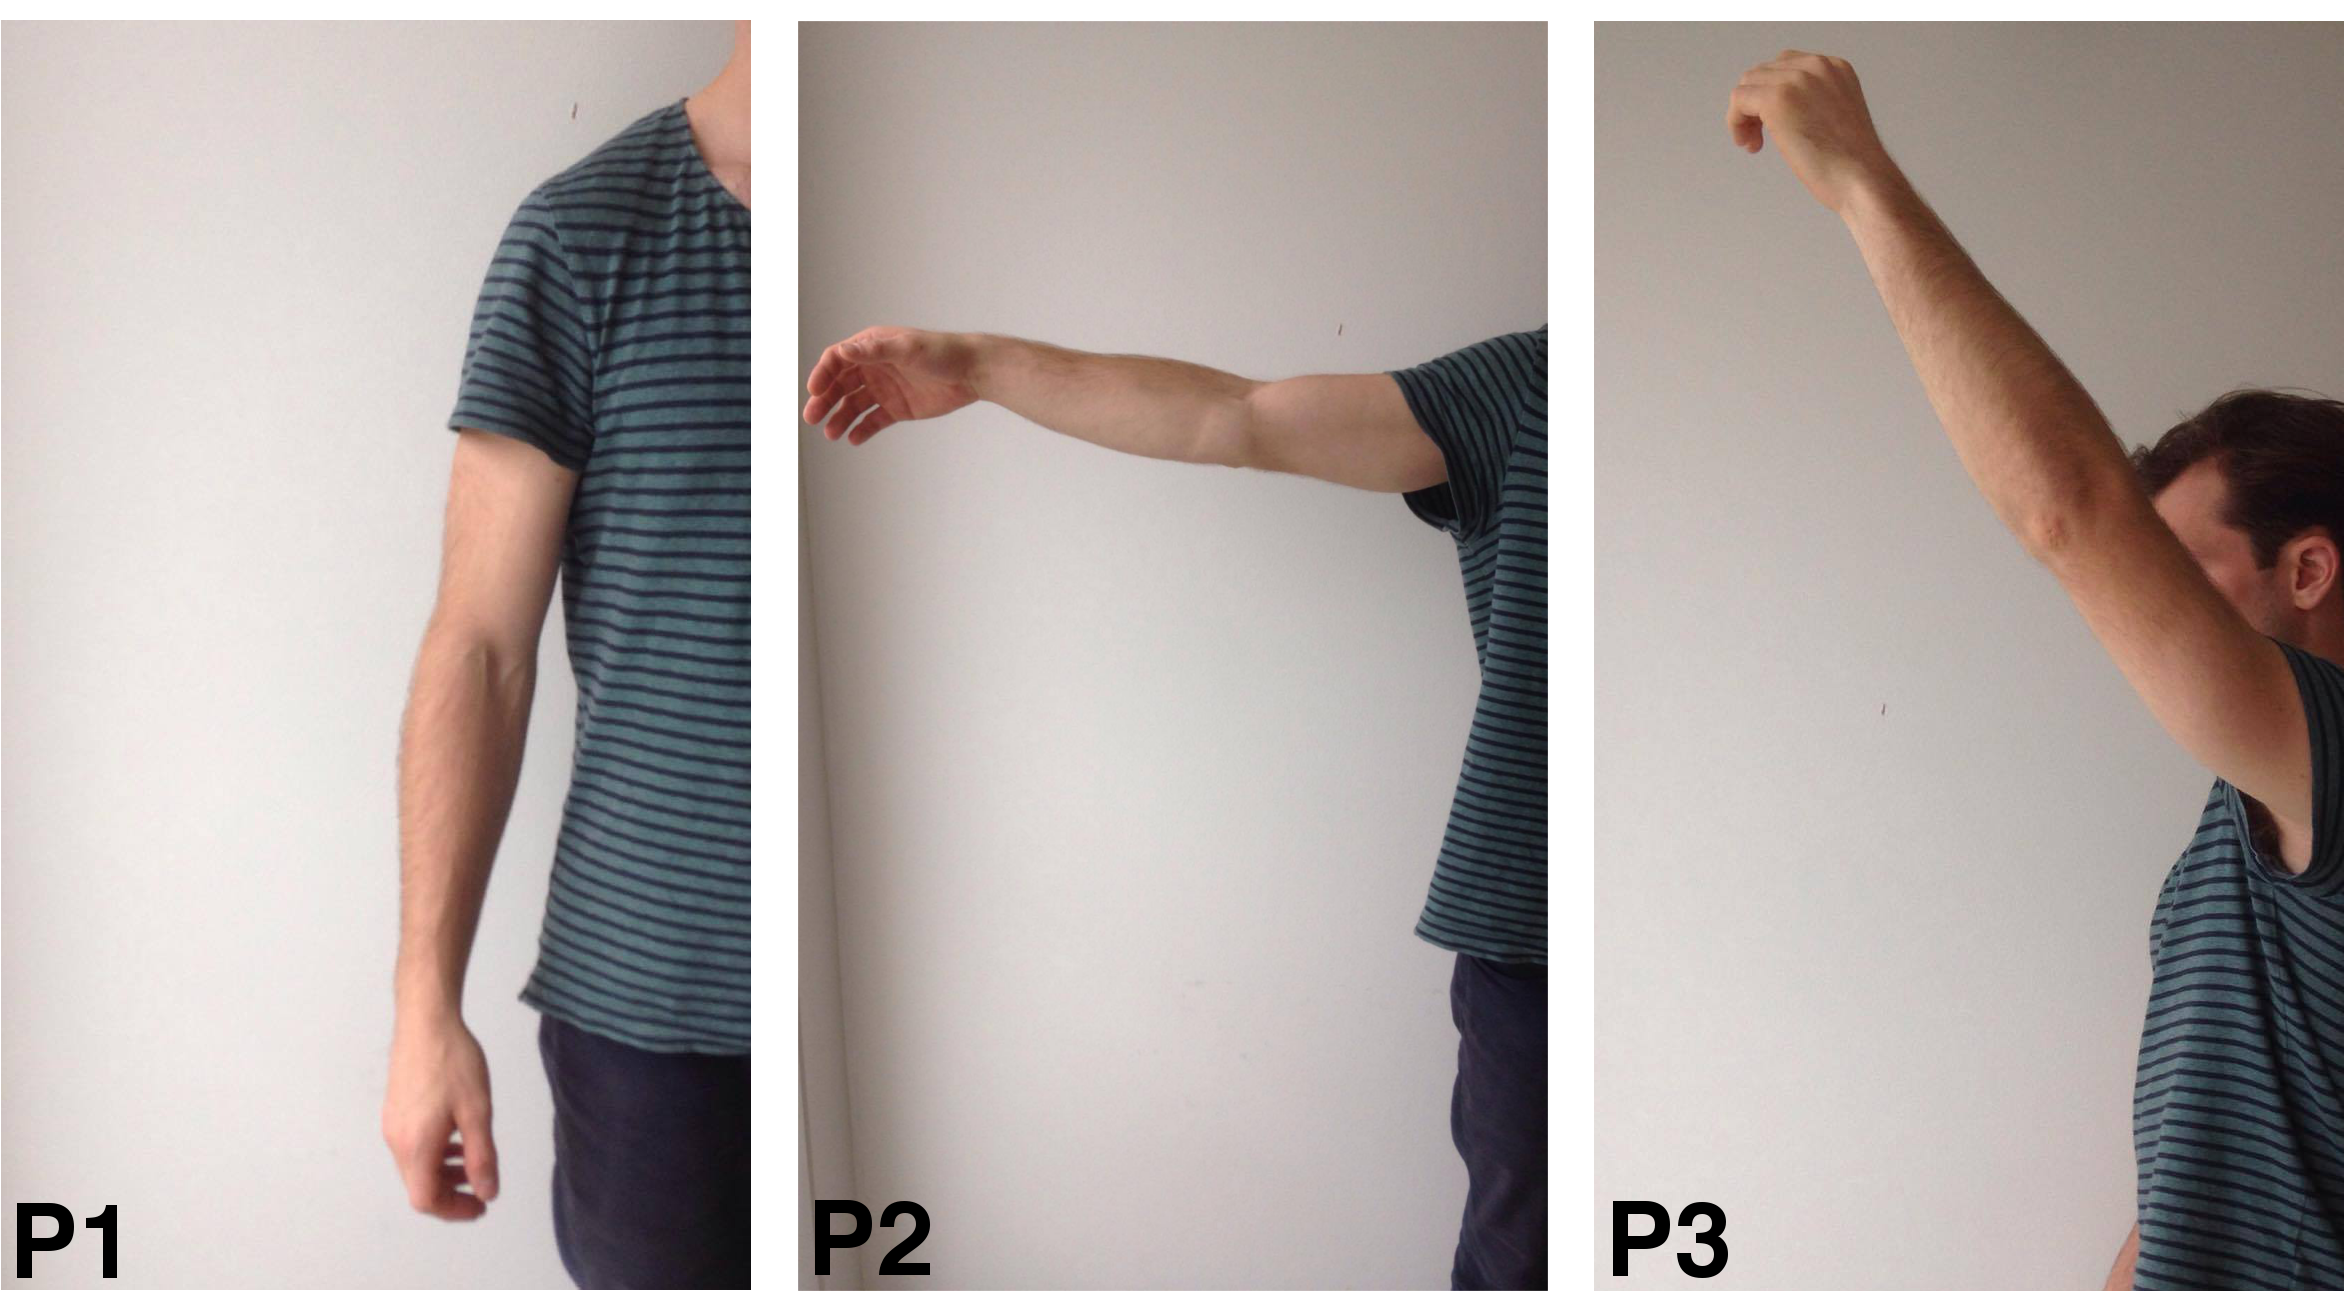
\includegraphics[width=1\textwidth]{figures/protocol/limb_positions}  %<--but is not needed.
	\caption{The limb positions consist of: 1) Relaxed arm hanging at the side of the torso, 2) straight arm reaching horizontally away from the torso and 3) straight arm reaching up 45 degrees from vertical.}
	\label{fig:limb_positions}  %<--give the figure a label, so you can reference!
\end{figure}

The subject will be given a relaxation period between trials in order to avoid shoulder fatigue.
Due to the fact that the hand gestures only consists of wrist movements, the subject must not move the fingers during the data acquisition.
The subjects will be in a standing position during the data acquisition procedure.
%time of rest?
Below is a table of the order at which each hand gesture will be performed, at which intensity and at which limb position. The table functions as a checklist for acquiring the training data.

%\begin{table}[h]
%	\centering
%\scalebox{.75}{
%		\begin{tabular}{|l|l|l|l|} 
%		\hline
%		& Limb 1 & Limb 2 & Limb 3  \\ \hline
%		\begin{tabular}[c]{@{}l@{}}Baseline\end{tabular} & & & & & \\ \hline
%		\begin{tabular}[c]{@{}l@{}}MVC\\ ulnar\end{tabular} & & & & & \\ \hline
%		\begin{tabular}[c]{@{}l@{}}25 \%\\ ulnar\end{tabular} & & & & & \\ \hline
%		\begin{tabular}[c]{@{}l@{}}50 \%\\ ulnar\end{tabular} & & & & & \\ \hline
%		\begin{tabular}[c]{@{}l@{}}75 \%\\ ulnar\end{tabular} & & & & & \\ \hline
%		\begin{tabular}[c]{@{}l@{}}MVC\\ radial\end{tabular} & & & & & \\ \hline
%		\begin{tabular}[c]{@{}l@{}}25 \%\\ radial\end{tabular} & & & & & \\ \hline
%		\begin{tabular}[c]{@{}l@{}}50 \%\\ radial\end{tabular} & & & & & \\ \hline
%		\begin{tabular}[c]{@{}l@{}}75 \%\\ radial\end{tabular} & & & & & \\ \hline
%		\begin{tabular}[c]{@{}l@{}}MVC\\ flex.\end{tabular} & & & & & \\ \hline
%		\begin{tabular}[c]{@{}l@{}}25 \%\\ flex.\end{tabular} & & & & & \\ \hline
%		\begin{tabular}[c]{@{}l@{}}50 \%\\ flex.\end{tabular} & & & & & \\ \hline
%		\begin{tabular}[c]{@{}l@{}}75 \%\\ flex.\end{tabular} & & & & & \\ \hline
%		\begin{tabular}[c]{@{}l@{}}MVC\\ ext.\end{tabular} & & & & & \\ \hline
%		\begin{tabular}[c]{@{}l@{}}25 \%\\ flex.\end{tabular} & & & & & \\ \hline
%		\begin{tabular}[c]{@{}l@{}}50 \%\\ flex.\end{tabular} & & & & & \\ \hline
%		\begin{tabular}[c]{@{}l@{}}75 \%\\ flex.\end{tabular} & & & & & \\ \hline
%		\begin{tabular}[c]{@{}l@{}}25 \%\\ ext.\end{tabular} & & & & & \\ \hline
%		\begin{tabular}[c]{@{}l@{}}50 \%\\ ext.\end{tabular} & & & & & \\ \hline
%		\begin{tabular}[c]{@{}l@{}}75 \%\\ ext.\end{tabular} & & & & & \\ \hline
%	\end{tabular}}
%
%	\caption{A checklist of the hand gestures each subject must perform and at which order.}
%	\label{tab:trainprotocol}
%\end{table}
\begin{table}[]
	\centering
	\caption{My caption}
	\label{my-label}
	\begin{tabular}{|l|l|l|l|}
		\hline
		& Limb 1 & Limb 2 & Limb 3 \\ \hline
		Baseline    &        &        &        \\ \hline
		MVC ulnar   &        &        &        \\ \hline
		25\% ulnar  &        &        &        \\ \hline
		50\% ulnar  &        &        &        \\ \hline
		75\% ulnar  &        &        &        \\ \hline
		MVC radial  &        &        &        \\ \hline
		25\% radial &        &        &        \\ \hline
		50\% radial &        &        &        \\ \hline
		75\% radial &        &        &        \\ \hline
		MVC flex.   &        &        &        \\ \hline
		25\% flex.  &        &        &        \\ \hline
		50\% flex.  &        &        &        \\ \hline
		75\% flex.  &        &        &        \\ \hline
		MVC ext.    &        &        &        \\ \hline
		25\% ext.   &        &        &        \\ \hline
		50\% ext.   &        &        &        \\ \hline
		75\% ext.   &        &        &        \\ \hline
	\end{tabular}
\end{table}
\section{Data Acquisition}

%head
The following section will include a description on how the data for the study have been acquired and processed. All data processing, along with GUI design and implementation, will be done in Matlab.

%presentaion of training GUI
To acquire data a training GUI has been designed and implemented in Matlab. The GUI has been designed to fulfil the specific needs for this project. An illustration of the GUI can be seen in \figref{fig:GUI_Training}. 

\begin{figure}[H]
	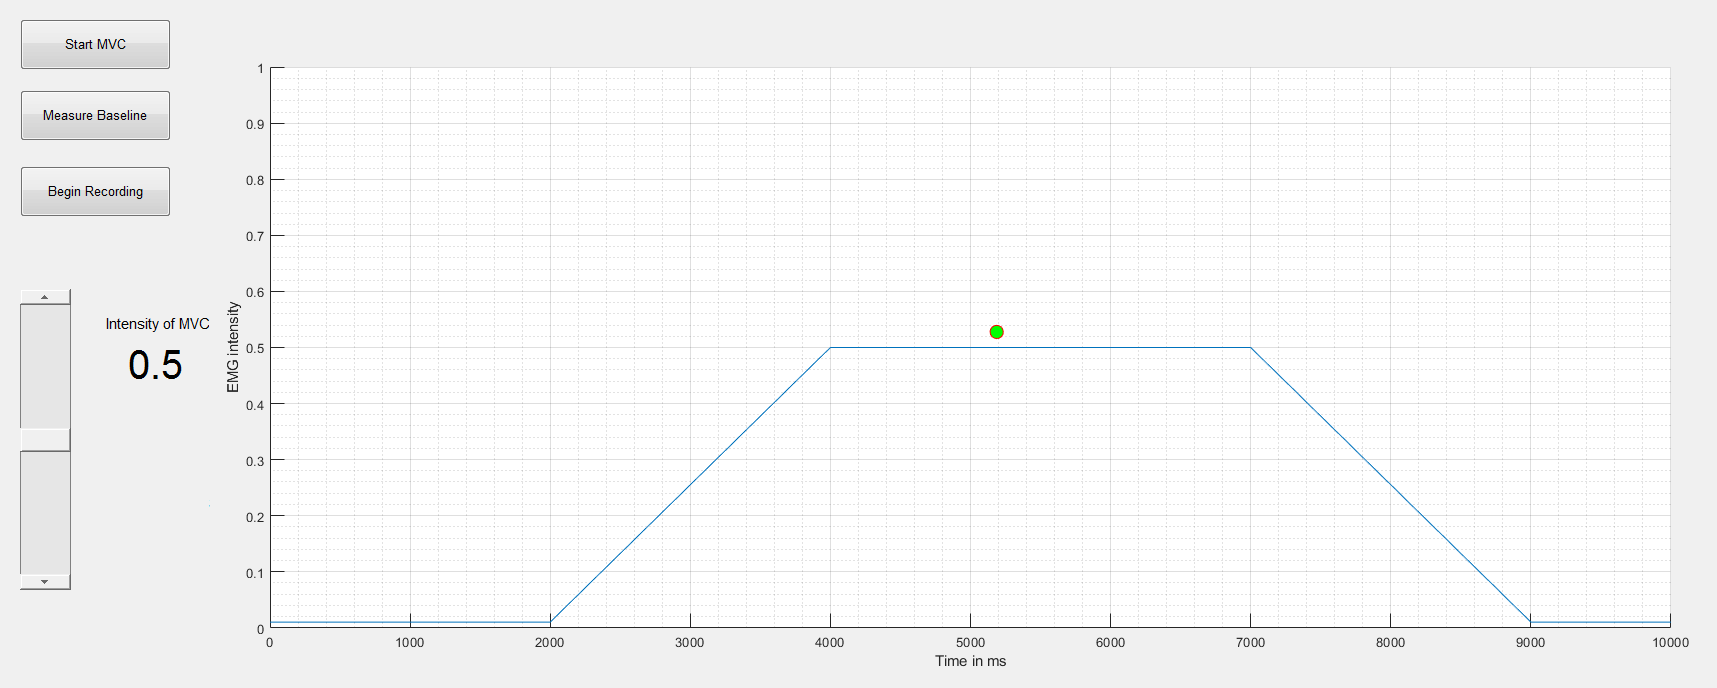
\includegraphics[width=.4\textwidth]{figures/GUI/GUI_Training.png}  %<--but is not needed.
	\caption{\textbf{WE GONNA NEED A NEW PIC OF THE GUI HERE} The training GUI implemented with Matlab GUI development environment. Control buttons to calculate MVC and perform MVC fraction recordings are placed on the left side. The trapezoid plot with the green dot controlled by the input EMG signal from the subject is shown on the right. The fraction of the MVC can be defined by the slider located under the control buttons.}
	\label{fig:GUI_Training}
\end{figure} 

The functions of the GUI consists of a baseline measurement button, a MVC measurement button, a data recording button and a fraction of MVC intensity slider. The baseline measurement is acquired for the purpose of being subtracted from the signal, in order to remove the signal artefacts that are present. At the baseline acquisition the subject is resting the lower arm in the given limb position. The MVC is calculated as a mean of the maximum values in each of the eight channels, and is set as a normalized reference point of 1. The MVC in a contraction at the intensity of which the subject can withhold for 15 seconds. The data recording contains the raw data of a fraction of the MVC. The slider must be set at the wanted fraction before the recording is started. The slider depicts a trapeze, where the plateau is the value the slider is set to. The trapeze depicts an initial resting phase of two seconds with the intensity of 0, a transition phase of two seconds with an ascending slope until the plateau phase is reached, which has a three second duration, and then a final descending transition phase of two seconds and resting phase of one second. Initialization of the recording will show a green dot, which moves with time on the x-axis and intensity on the y-axis normalized from 0 to 1. The green dot is calculated as the mean of the input EMG signal in a 200 ms window, where each window has an overlap of 100 ms. The signal is afterwards normalized with the MVC measurement as the reference point. From this acquired data features will be extracted and used to train regressors for each of the subjects for each of the hand gestures performed.



%presentation of acquired data

%maybe in the results section(?): differences between the regressors recognizing a movement when they have been trained using log-var and MAV





\section{Feature extraction}
In this section it will be explained which features that are extracted from the EMG data.\\
A commonly used feature in control of prosthetics is the MAV. The equation of MAV is as follows:

\begin{equation}
MAV = \frac{1}{N}\sum\limits_{i=1}^N|x_i|
\end{equation}

As the equation and name indicates MAV is the average of the absolute values of the EMG signal, where N is the length of the sample window, and $x_i$ is the $i^{th}$ sample of the signal. \\
According to a study by Hahne et al. \cite{hahne2014}, the variance of a signal has exponential properties, but taking the logarithm of it ($log(\sigma^2)$), gives it linear properties. This linearity might yield a better estimation in the recognition of the hand gestures since linear regression is used to as the mapping tool of the hand gestures. The LogVar feature is calculated as in \eqref{eq:logvar}:

\begin{equation} \label{eq:logvar}
log(\sigma^2) = log(\frac{\sum\limits_{i=1}^N(x_i - \mu)^2}{N})
\end{equation}

where $N$ is the length of the sample window, $x_i$ is the $i^{th}$ sample of the signal and $\mu$ is the mean. The logarithmic variance calculates the logarithm of the variance, which is the sum of the squared deviation of a variable from its mean. Thus, how spread the signal is from its average.

% for the logarithmic variance to be extracted as a feature in this project, along with the MAV. 

%Comparison of the linear properties of the features mean absolute value and logarithmic variance.
%Visualize it with a polynomial plot of the different hand gestures with the intensities in prolongation of each other. The x-axis will be the normalized EMG signal and the y-axis will be the ideal values(trapeze plateaus).
\subsection{Validation of data}

%collect data (described earlier)
%review data to evaluate if the acquired data is valid for training the regressors
%do PCA to validate data (qualitatively) -> t-test (only later if we are fast) to check if data clouds are significalnty different from each other
%if data is different: good. if data not different: bad, redo data acquisition
%do training of regressors (next section)

After features has been extracted from the data, the feature data is validated through Principal Component Analysis (PCA) to determine the quality of the recorded data in the sense of identify outliers and examining whether the data from the different hand gestures are distinguishable. Thus, the PCA will only be used as a qualitative tool to validate the data. %due to lack of time
%include if we are fast
%and t-test to decide if there are any significant outliers and if the features are significantly different from feature data of other movements. The PCA is used to determine the relation between the feature data and identifying data outliers. 
%What is PCA?
PCA is an analysis tool used to express a set of correlated variables into non-correlated components, such that the dataset can be expressed in a reduced dimensionality hyperspace using less variables, however more defining variables for the given data set. These variables are called the principal components. Each PC is orthogonal on the former, meaning that they each define the largest variance in an axis, different from axes described by other components. PCA also provides knowledge on which components are the most defining for the dataset, where the first vectors in the hyperspace being the ones with highest variance, so only the most important can be considered. When performing PCA it provides the coefficients of the principal components (PCC), which can be visualised in a plot. This plotting of the coefficients are what is used to evaluate the quality of the feature data. A threshold of 90\% for preserved information is used. 

PCA is performed for each movement in each limb position and plotted in a three dimensional space. If the PCC's of a movement has significant outliers, or the points are clustered, it will be identified shortly after the feature extraction, and a new recording session for the test subject can be executed to prevent inaccurate training of regressors and time delays. If the data is of high quality, meaning the clouds of data points are easily distinguishable from each other, it can be used further on to train the regressors.

\begin{figure}[H]
	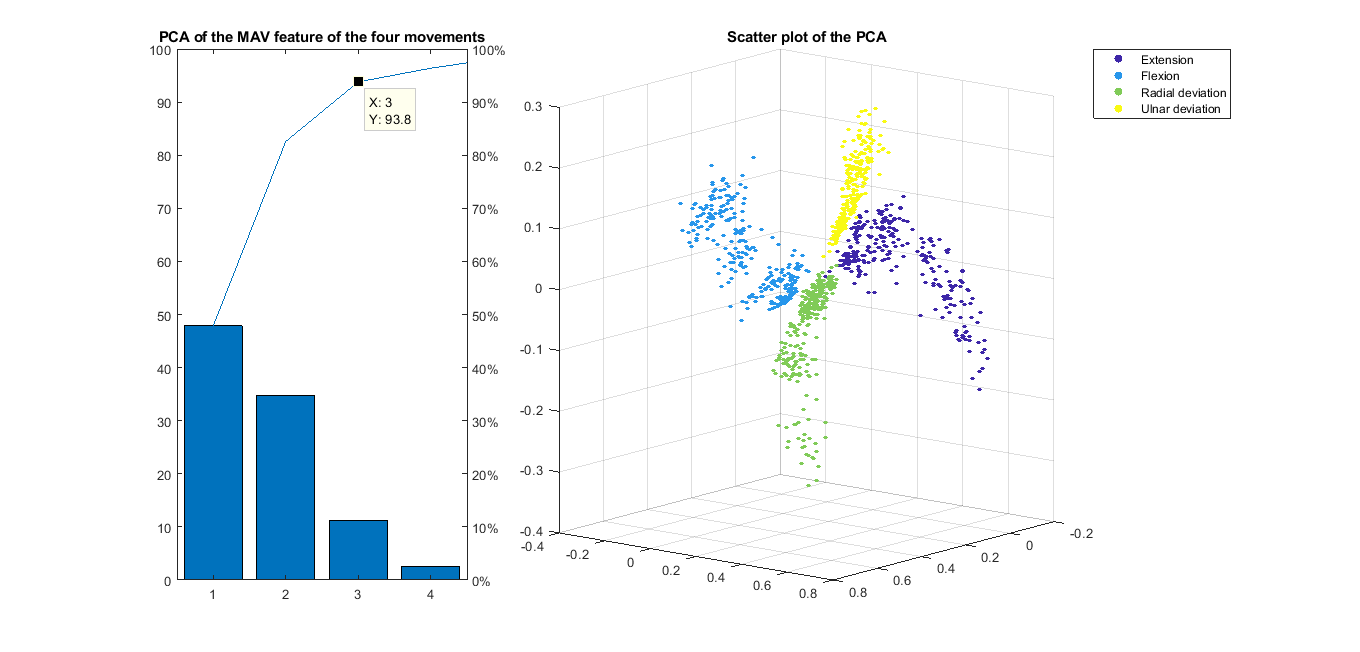
\includegraphics[width=.4\textwidth]{figures/Methods/pcasubplot.png} 
	\caption{Plot of PCA. To the left the first four principal components are visualised. The first three principal components account for describing $93.8\%$ of the data set. On the right the PCC's are plotted for each movement. The clusters for each movement are distinguishable from each other and have no noteworthy outliers, so the data is considered of high quality.} 
	\label{fig:pcasubplot}
\end{figure} 

In \figref{fig:pcasubplot} an example of a PCA performed on feature data from one test subject is shown. The left plot of the principal components describe the importance of each identified components, and how much of the variance in the data that is described. Using only the first three components, $93.8\%$ of the full dataset can be described. Only these principal components are used in the plot to the right in \figref{fig:pcasubplot}. Here it can be seen that the clusters are easily distinguishable and have no remarkable outliers. Therefore the data is considered good and can be used in the training of the regressors.






\section{Regression model}
%Preprocessing
%Feature extraction

%regression
%This section will include a description of how the regression methods have been executed. As well as data gathering and processing, the regression model will be implemented in MATLAB.

Once the preprocessing and the feature extraction of the EMG data has been done, regression will be used as described in \secref{sec:regressionMethods}. The implementation follows multivariate linear regression as shown in \eqref{eq:multiLinearRegression}. As mentioned in \secref{sec:dataAcquisition} one regressor will be trained for each subject for each of the hand gestures performed. 

For each subject the extracted feature data from the eight sEMG channels will be mapped to estimate a movement. Because multivariate regression is used there will be an estimated output for each of the input variables (each of the eight channels). These outputs are expressed by one hyperplane, which is the output for the regressor. Each subject will then have four regressors trained, one for each movement. 
To train the regressors an input matrix will be constructed. This matrix will contain all the extracted features from all eight channels, for all recorded movements, for all intensities, in all three limb positions. The matrix will be structured into segments, where each segment contains data from one movement. One segment will be structured as shown in \eqref{eq:segMatrix}, with the feature data of a movement during 30\% contraction in one limb position first, followed by 30\% contraction for the same movement in the second limb position, and so on. This is true for all contraction intensities (30\%, 50\%, 80\%).

\begin{equation} \label{eq:segMatrix}
\begin{bmatrix} 
\ Flex30Down_{1,1}, Flex30Down_{1,2} \cdots Flex30Down_{1,8} \\ 
\ \vdots \qquad \qquad \qquad \ddots \qquad \qquad \qquad \vdots \\
\ Flex30Down_{n,1}, Flex30Down_{n,2} \cdots Flex30Down_{n,8} \\
\ Flex30Side_{o,1}, Flex30Side_{o,2} \cdots Flex30Side_{o,8} \\
\ \vdots \qquad \qquad \qquad \ddots \qquad \qquad \qquad \vdots \\
\ Flex30Side_{p,1}, Flex30Side_{p,2} \cdots Flex30Side_{p,8} \\
\ Flex30Up_{q,1}, Flex30Up_{q,2} \cdots Flex30Up_{q,8} \\
\ \vdots \qquad \qquad \qquad \ddots \qquad \qquad \qquad \vdots \\
\ Flex30Up_{r,1}, Flex30Up_{r,2} \cdots Flex30Up_{r,8} \\
\ Flex50Down_{s,1}, Flex50Down_{s,2} \cdots Flex50Down_{s,8} \\
\ \vdots \qquad \qquad \qquad \ddots \qquad \qquad \qquad \vdots \\
\ \vdots \qquad \qquad \qquad \ddots \qquad \qquad \qquad \vdots \\
\ Flex80Up_{t,1}, Flex80Up_{t,2} \cdots Flex80Up_{t,8} \\
\end{bmatrix}
\end{equation}

The input matrix will then consist of four segments, one for each movement in all three limb positions, as shown in \eqref{eq:featDataMatrix}:

\begin{equation} \label{eq:featDataMatrix}
\begin{bmatrix} 
\ Flex_{1,1}, Flex_{1,2} \cdots Flex_{1,8} \\ 
\ \vdots \qquad \ddots \qquad \vdots \\
\ Flex_{n,1}, Flex_{n,2} \cdots Flex_{n,8} \\
\ Exte_{o,1}, Exte_{o,2} \cdots Exte_{o,8} \\
\ \vdots \qquad \ddots \qquad \vdots \\
\ Exte_{p,1}, Exte_{p,2} \cdots Exte_{p,8} \\
\ Radi_{q,1}, Radi_{q,2} \cdots Radi_{q,8} \\
\ \vdots \qquad \ddots \qquad \vdots \\
\ Radi_{r,1}, Radi_{r,2} \cdots Radi_{r,8} \\
\ Ulna_{s,1}, Ulna_{s,2} \cdots Ulna_{s,8} \\
\ \vdots \qquad \ddots \qquad \vdots \\
\ Ulna_{t,1}, Ulna_{t,2} \cdots Ulna_{t,8} \\
\end{bmatrix}
\end{equation}

%The feature data will be constructed into one matrix containing the extracted features for all four movements at all intensities including the baseline in the three different limb positions arranged into four segments in the matrix. 

This matrix \eqref{eq:featDataMatrix} including the baseline recordings, will be set as input to the training of the regressor. The output for training the regressors are set to the desired values for the performed movement. The desired values are the mean of the data from all eight channels when the subject traced the trapezoid during data acquisition, as shown on \figref{fig:GUI_Training} in \secref{sec:dataAcquisition}. The data is scaled in relation to the MVC for the subject and are structured in a vector with segments of data for each movement similar to that of the matrix \eqref{eq:featDataMatrix} containing the feature data. When training a regressor for a movement, the desired values for the segments in the output vector corresponding to the movements that are not being trained, are augmented with zeros. This ensures that the trained regressor will estimate zero when recognising movements other than the one movement it is trained to recognise. 

%, while the estimator is a vector containing the mean of all eight channels of the actual data, normalized in relation to the recorded MVC. This provides data for the movement that the regressor will be trained to recognize. The estimator vector is augmented with zeros for the segments of the movements that the regressor is trained not to recognize. This is shown in \eqref{eq:regressionMatrix}
%
%\begin{equation} \label{eq:regressionMatrix}
%\begin{bmatrix} 
%\ normMove_1 \\ 
%\ \vdots\\
%\ normMove_n\\
%\ 0_o\\
%\ \vdots\\
%\ 0_p\\
%\end{bmatrix}=
%\alpha +
%\begin{bmatrix}
%\ \beta_1\\
%\ \vdots\\
%\ \beta_8\\
%\end{bmatrix} \cdot
%\begin{bmatrix} 
%\ rightFeat_{1,1} \cdots rightFeat_{1,8} \\ 
%\ \vdots \qquad \ddots \qquad \vdots \\
%\ rightFeat_{n,1} \cdots rightFeat_{n,8} \\
%\ wrongFeat_{o,1} \cdots wrongFeat_{o,8} \\
%\ \vdots \qquad \ddots \qquad \vdots \\
%\ wrongFeat_{p,1} \cdots wrongFeat_{p,8} \\
%\end{bmatrix}
%\end{equation}
%
%Where \textit{normMove} is the desired estimator, \textit{rightFeat} is the desired input feature for the desired movement in all limb positions and \textit{wrongFeat} is the features that should not be recognized by the given regressor. 

The regressor is implemented through the Matlab function \textit{fitlm}, which use the input matrix and estimator vector to calculate the slope and intercept of the regressor, according to \eqref{eq:multiLinearRegression} in \secref{sec:regressionMethods}.
This procedure is done for each movement, which yields four regressors trained to recognize one movement each. This procedure is done individually for MAV and LogVar, to compare the accuracy and performance between the two features. 

When implementing the IMU data three extra columns are added to the input matrix, because the accelerometer provides a three axis output during recordings. The raw accelerometer data is used. New regressors are trained for each subject similar to the described procedure, including the IMU data and is compared to the regressors trained with only the EMG feature data. 


%
%
% In order to implement this in MatLab the function \textit{fitlm} will be used to build the regressors. 
%
%
%it is needed to apply regression methods to determine the relationship between the variables under study, since the objective of a regression methods is mapping the response as a function of the predictions. \cite{hahne2014}
%
%In this particular study, a simple linear regression has been applied. The equation is:
%
%\begin{equation} %\label{eq:simpleLinearRegression}
%Y_i = \alpha + \beta X_i + \epsilon_i
%%\label{reg}
%\end{equation}
%
%where, $Y$ is the dependent variable or response, $X$ is the independent variable or the predictor, $\beta$ is the regression coefficient or the slope, and $\alpha$ is the Y intercept,  $\epsilon$ is the error and $i$ is the index.\cite{zar2009}.
%
%%capital letters matlab
%There has been implemented four different regressors, one for each movement under study. MATLAB is able to generate a linear regression model with one of its build-in mathematical functions. In order to accomplish the regressor the given training data set should include the predictions and the responses.
%The equation which implements the regressor is given in \ref{regressor}. Where Y contains the outputs or the target, this is the response recorded during the training session through the GUI. The values were normalize obtaining an optimal value between 0 and 1. X contains the inputs, in this case, the features extracted from each of the eight channel of the Myo armband. The features extracted from the recorded EMG data were the mean absolute value $\left( MAV\right)$ and  the logarithmic variance. %due to its better performance \cite{hahne2014}. 
%\begin{equation}
%	Y_i=\begin{bmatrix} 
%	\ norm_1 \\ 
%	\ norm_2\\ 
%	\ \vdots\\
%	\ norm_8\\
%	\end{bmatrix}=
%	\alpha +
%	\begin{bmatrix} 
%	\beta_1 \; \beta_2 \cdots \beta_8\\ 
%	\end{bmatrix}
%	\cdot 
%		\begin{bmatrix} 
%	\ X_1 \\ 
%	\ X_2\\ 
%	\ \vdots\\
%	\ X_8
%	\label{regressor}
%	\end{bmatrix}
%\end{equation}
%
%

\section{Accuracy of regressors}

%head
This section will cover the test used to determine the accuracy of the trained regressors. Both methods are performed on the regressors trained with only EMG data and when IMU data is combined with the EMG data. 

\subsection{Superimposition}
To examine how well the regressors fit the actual data, the output of the regressors build for each feature is superimposed on the actual data. It can then be shown how the regressors perform at which intensities and which movements, and whether other regression methods should be considered to obtain a lower error.  


\subsection{Root Mean Square Error}
To measure the accuracy of the regressors the Root Mean Square Error(RMSE) is calculated. RMSE is a measure to examine how much the regressors disagrees with the actual data. RMSE a calculation of the standard deviation of the residuals, which is the difference between the estimated values and the actual values. The RMSE is calculated as follows:

\begin{equation}
RMSE = \sqrt{\frac{\sum\limits_{i=1}^N(y_i - \hat{y_i})^2}{N}}
\end{equation}

Where N is the length of the signal, $y_i$ is the $i^th$ variable of the actual data and $\hat{y_i}$ is the $i^th$ output of the regressor. The RMSE will be done for the regressor of each movement.

To express that the regressors do not overfit the input data, the RMSE of the test data must be lower than or equal to the training data. It does not necessarily express a great performing model if the RMSE of the training data is high, but a model that performs consistently on new data. However, if the RMSE of the training is reasonably low, and the RMSE of the test data is likely low, the model is said to fit the data well. 


%\section{Test GUI}

As a means to express the movement recognition of the trained regressors, a test GUI has been implemented to confirm that the regressors are trained accordingly and translate to a specific direction. Furthermore, the test GUI serves as a digital way to test the system before moving on the controlling the JACO robotic arm. 

\begin{figure}[H]
	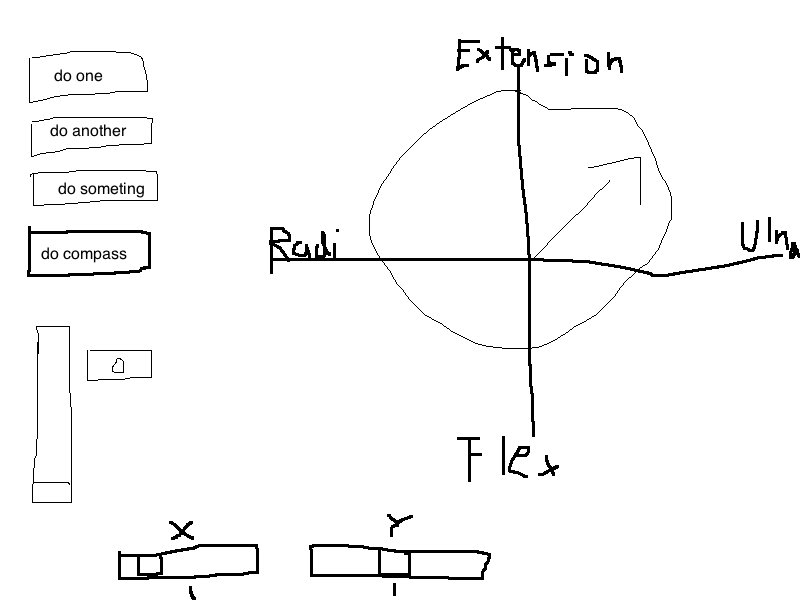
\includegraphics[width=.4\textwidth]{figures/GUI/GUI_test.png}  %<--but is not needed.
	\caption{The test GUI. The compass plot shows the movement and intensity of the EMG, as recognised by the regressor, by arrow direction and length. The test GUI is implemented in the same GUI as the training GUI and will change the plot type once the correct button is pressed.}
	\label{fig:testGUI}
\end{figure}

As seen in \figref{fig:testGUI} the test GUI consists of a compass-like plot with captions for the four movements in four different direction. The compass-plot will illustrate the performed movement by an arrow pointing in the direction of the movement with the intensity of the movement shown as the length of the arrow. The compass-plot have been made so the directions are intuitive in relation to performed movements of the hand, with the palm of the hand facing down as starting point. This is not necessary according to Ison et al. \cite{Ison2016}, as non-intuitive control schemes are not a barrier in learning proper control of prosthetics. The control scheme might change when adapting to system for control of the JACO robotic arm. Sensitivity sliders are implemented in the GUI to enable fine tuning of the intensity to make valid plotting of the arrow in the (X,Y) directions, in case the regressor values are too small to make a proper plot. 
The compass plot will continuously update to plot the direction of the movement and intensity. 
%\section{Fitts' Law}

Fitts' Law will be used to quantify the versatility of the regressors. Fitts' Law is a predictive model describing the relation that the time it takes to do a rapid movement to reach a target area, is dependent on the distance to the target area, and the size of the target area. The law demonstrates that the information of any human motor tasks, is finite and only limited by the capabilities of the control system. The control exhibit a negative correlation between speed and accuracy. \cite{Kamavuako2014}
Fitts' Law calculates an \textit{Index of Difficulty} (ID) by \eqref{eq:Fitts}

\begin{equation} \label{eq:Fitts}
$ID = log_{2} * (\frac{2D}{W}) \ \ \ \ \ , where ID is Index of Difficulty, D is distance to targes, W is width of target area.
\end{equation}

To calculate the performance of the human interacting with the control system, the \textit{throughput} (TP) was introduced. IP is calculated by \eqref{eq:TP}.

\begin{equation} \label{eq:TP}
$TP = \frac{ID}{MT} \ \ \ \ \ , where ID is Index of Difficulty, MT is movement time.
\end{equation}

MT is the time it would take a subject to move a pointer from origin to the target area.

Fitts' Law will be implemented into the test GUI described in \secref{sec:testGUI}, where it will test the control systems ability to correctly convey the test subjects task of reaching points in the compass-plot. 



\chapter{Results}
\section{Separability of data}
%results PCA

PCA is performed on all feature data from each test subject for both MAV and logarithmic variance features. As described in \secref{sec:dataValidation} the PCA is only used as a tool to qualitatively evaluate the data. In \figref{fig:pcasubplotMAV} a PCA is shown from one test subject, performed with the MAV feature. 

\begin{figure}[H]
	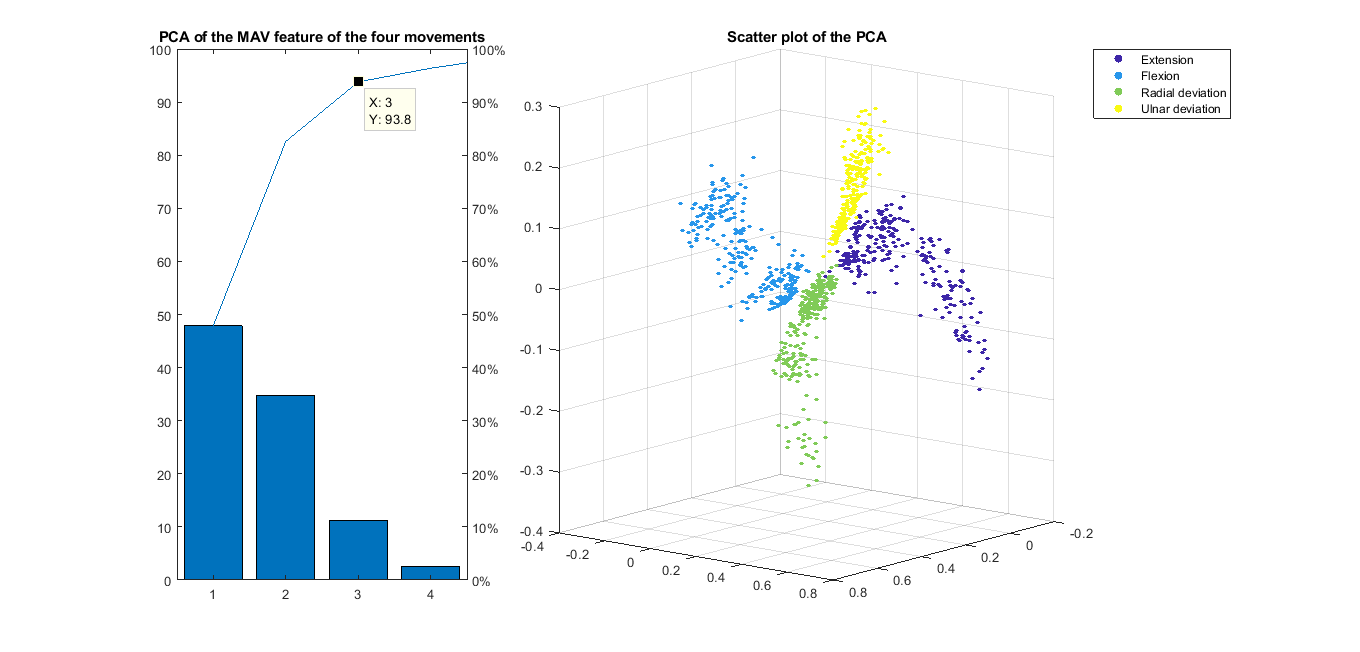
\includegraphics[height=0.2\textheight,width=1.1\textwidth]{figures/results/pcasubplotMAV.png} 
	\caption{Plot of PCA of MAV feature. To the left are the amount of data that the first four principal components describe expressed in percentage. The first three principal components account for describing $93.8\%$ of the data set. On the right are the data described by the first three principal components plotted for each movement. The clusters for each movement are distinguishable from each other and have no noteworthy outliers, so the data is considered of high quality.} 
	\label{fig:pcasubplotMAV}
\end{figure} 

\begin{figure}[H]
	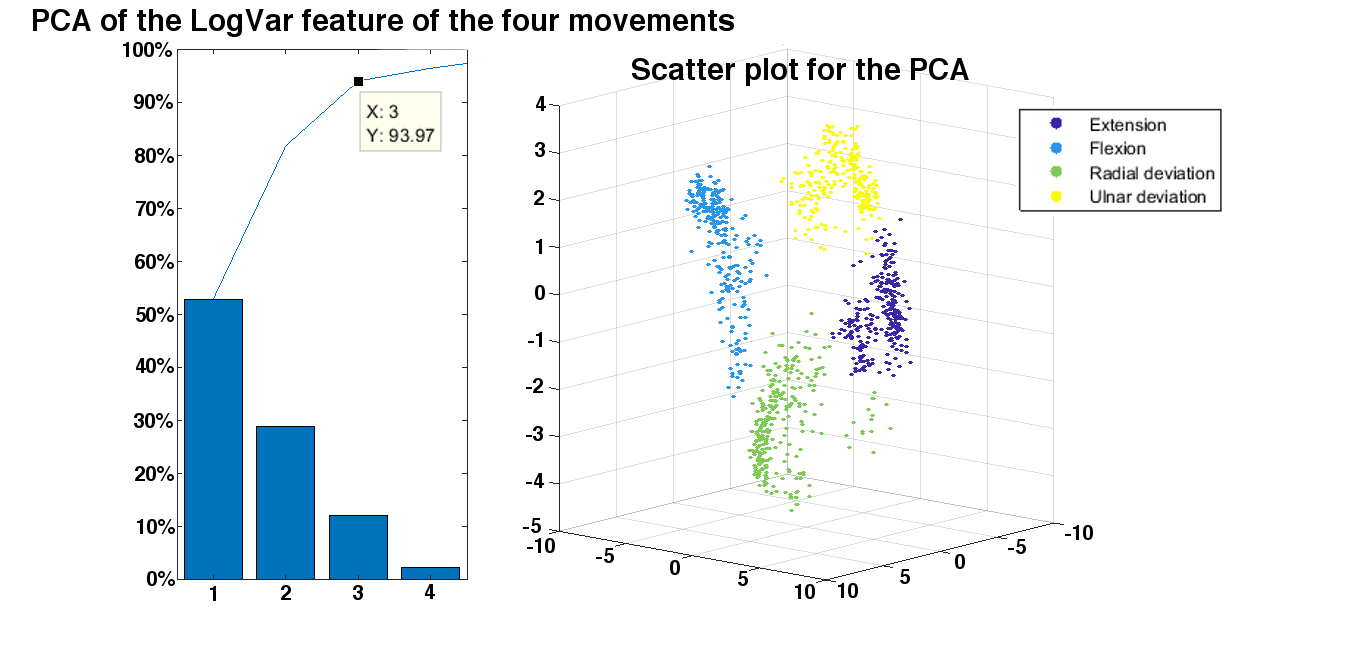
\includegraphics[height=0.2\textheight,width=1.1\textwidth]{figures/results/pcasubplotLogVar.png} 
	\caption{Plot of PCA of logarithmic variance feature. The first three principal components account for describing $93.97\%$ of the data set. Here the clusters for each movement are also distinguishable from each other and have no noteworthy outliers, so the data is considered of high quality.} 
	\label{fig:pcasubplotLogVar}
\end{figure}

The left plot of the principal components describe the importance of each identified components, and how much of the variance in the data that is described. For the MAV feature depicted in \figref{fig:pcasubplotMAV}, using only the first three components, $93.8\%$ of the full dataset can be described. Only these principal components are used in the plot to the right in both figures. The same is the case for the PCA of logarithmic variance shown in \figref{fig:pcasubplotLogVar}, where the first three PC's account for describing $93.97\%$ og the data. In both PCA's it can be seen that the clusters are easily distinguishable and have no remarkable outliers. Therefore the data is considered good and can be used in the training of the regressors.


%same with IMU data

\section{Regression accuracy}
This section includes an examination of the accuracy of the regressors. This will be examined through superimposition of the regressor outputs on the estimated data, and through RMSE plots. To evaluate how the regressors perform with new data, a test with new data of 50 $\%$ of the MVC of all movements in all limb positions will be fed the regressor and the above examination of accuracy will be performed. 

The plot in \figref{fig:SuperPositionTestDataLogVar} depicts the actual data superimposed on the estimated data from the regressors trained with the logarithmic variance features. 

\begin{figure}[H]
	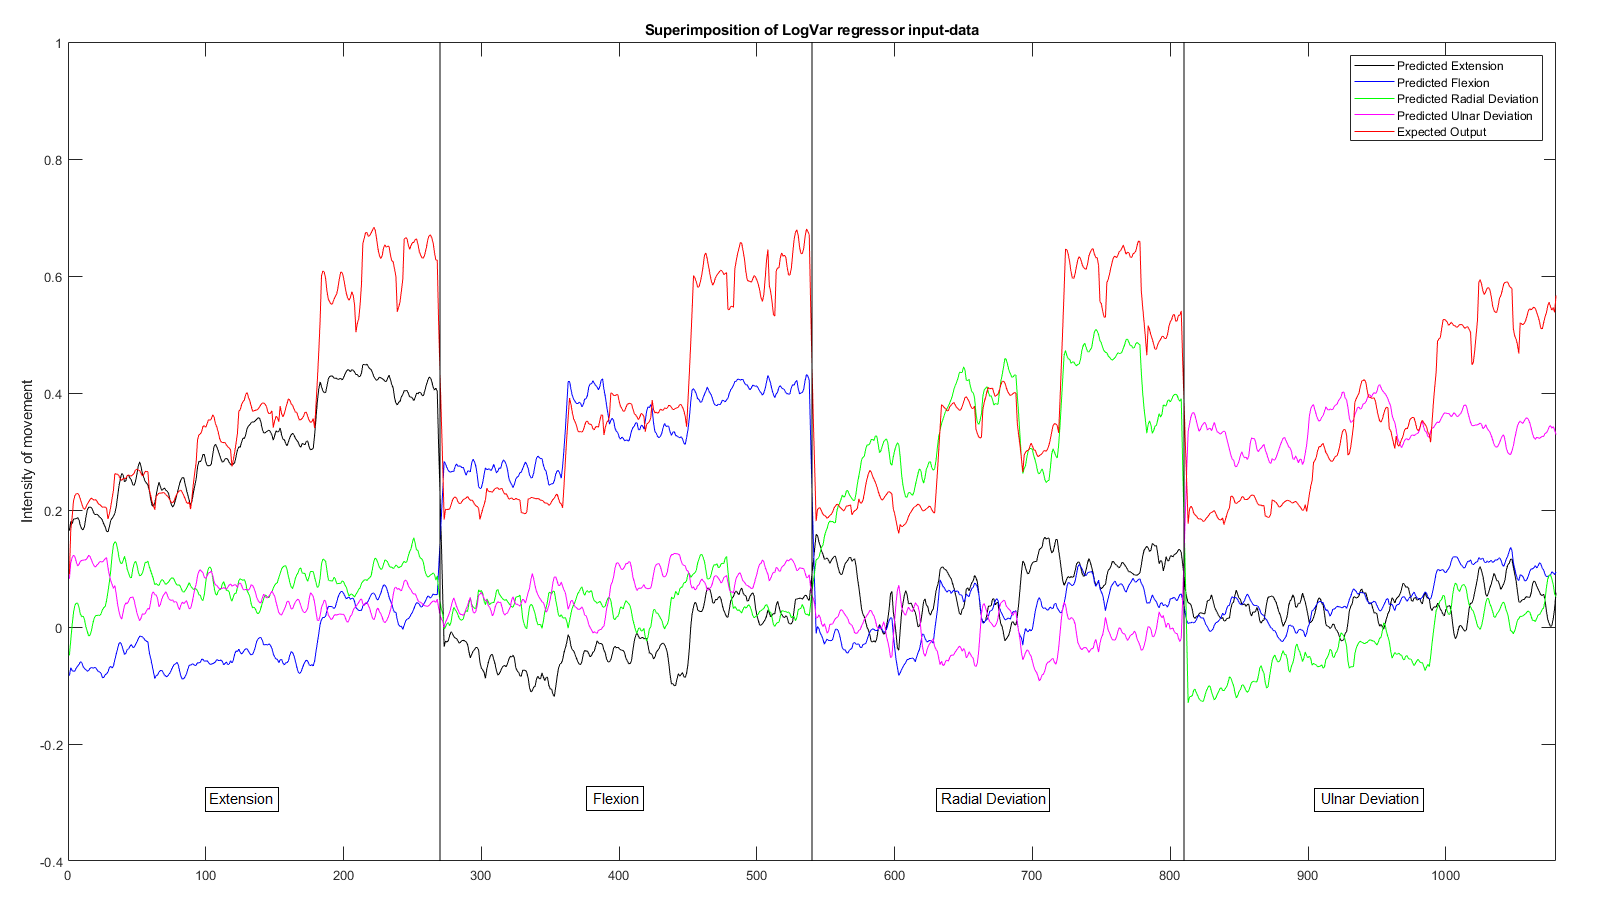
\includegraphics[width=0.7\textwidth]{figures/results/SuperPositionTestDataLogVar}  %<--but is not needed.
	\caption{Plot of the actual data, red plot, superimposed on the output of the regressors trained with the logarithmic variance features. The plot is divided into four segments, where each segment shows a different movement performed. Each segment has the same sample size.}
	\label{fig:SuperPositionTestDataLogVar}  %<--give the figure a label, so you can reference!
\end{figure}

The plot in \figref{fig:SuperPositionTestDataMAV} depicts the actual data superimposed on the estimated data from the regressors trained with the MAV features. 

\begin{figure}[H]
	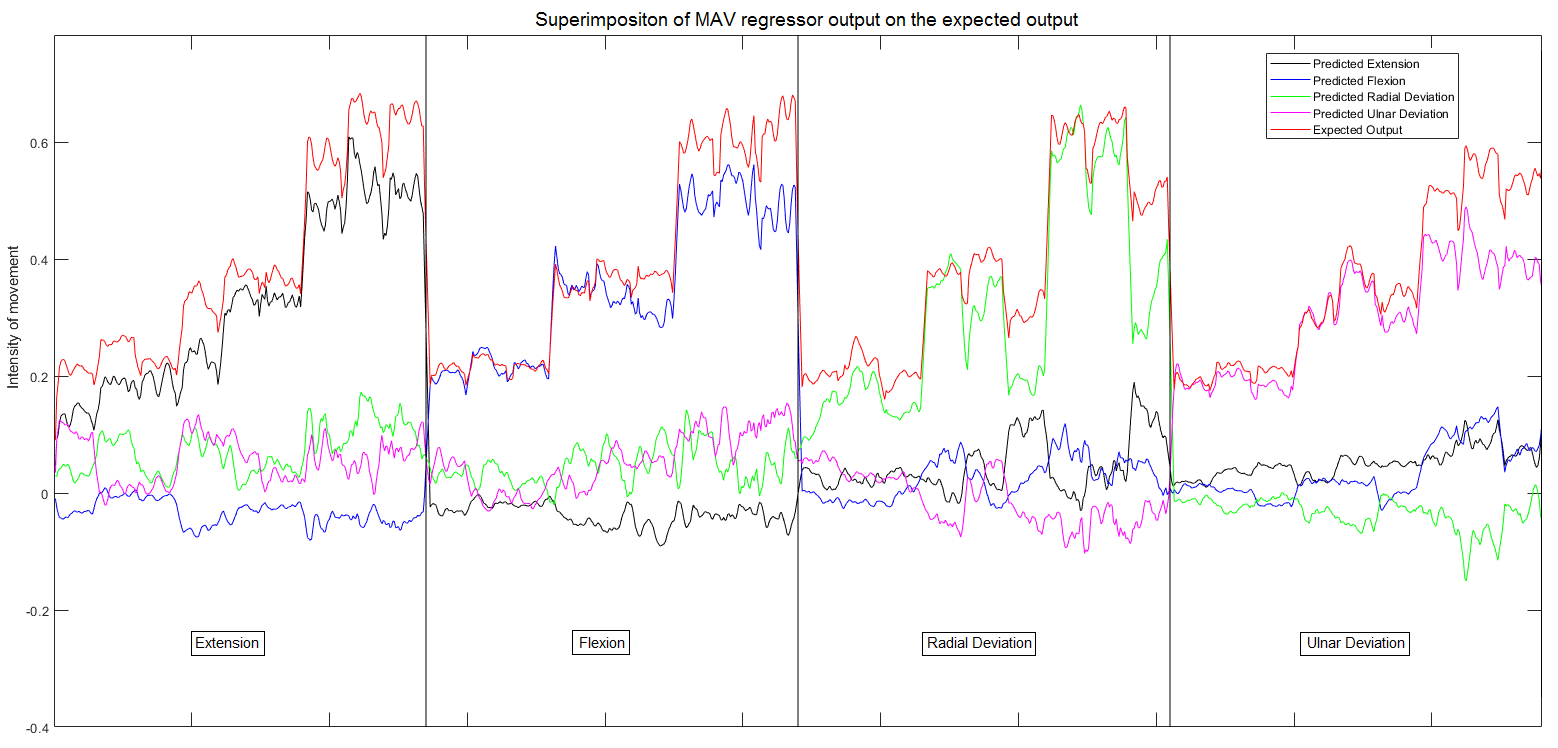
\includegraphics[width=0.7\textwidth]{figures/results/SuperPositionTestDataMAV}  %<--but is not needed.
	\caption{Plot of the actual data, red plot, superimposed on the output of the regressors trained with the MAV features. The plot is divided into four segments, where each segment shows a different movement performed. Each segment has the same sample size.}
	\label{fig:SuperPositionTestDataMAV}  %<--give the figure a label, so you can reference!
\end{figure}


A qualitative examination of the plots shows that each regressor reacts on the movement it is fitted for, and remains inactive when another movement is performed. This accounts for both features. Both regressors has a lower accuracy in the high intensities, especially for the regressors trained with logarithmic variance features. 
%regression on MAV features yields a more accurate output than regression on the logarithmic variance feature, whereas both estimates yield inaccurate fitting in the high intensities. However, both estimates yield inaccurate fitting in the high intensities compared to the lower intensities, especially in the ulnar deviation movement.
  


Calculating the RMSE of the regressors for the MAV and logarithmic variance features of the training data across all subjects, yields the results depicted in \figref{fig:gimmeThemRMSEBars}. 

\begin{figure}[H]
	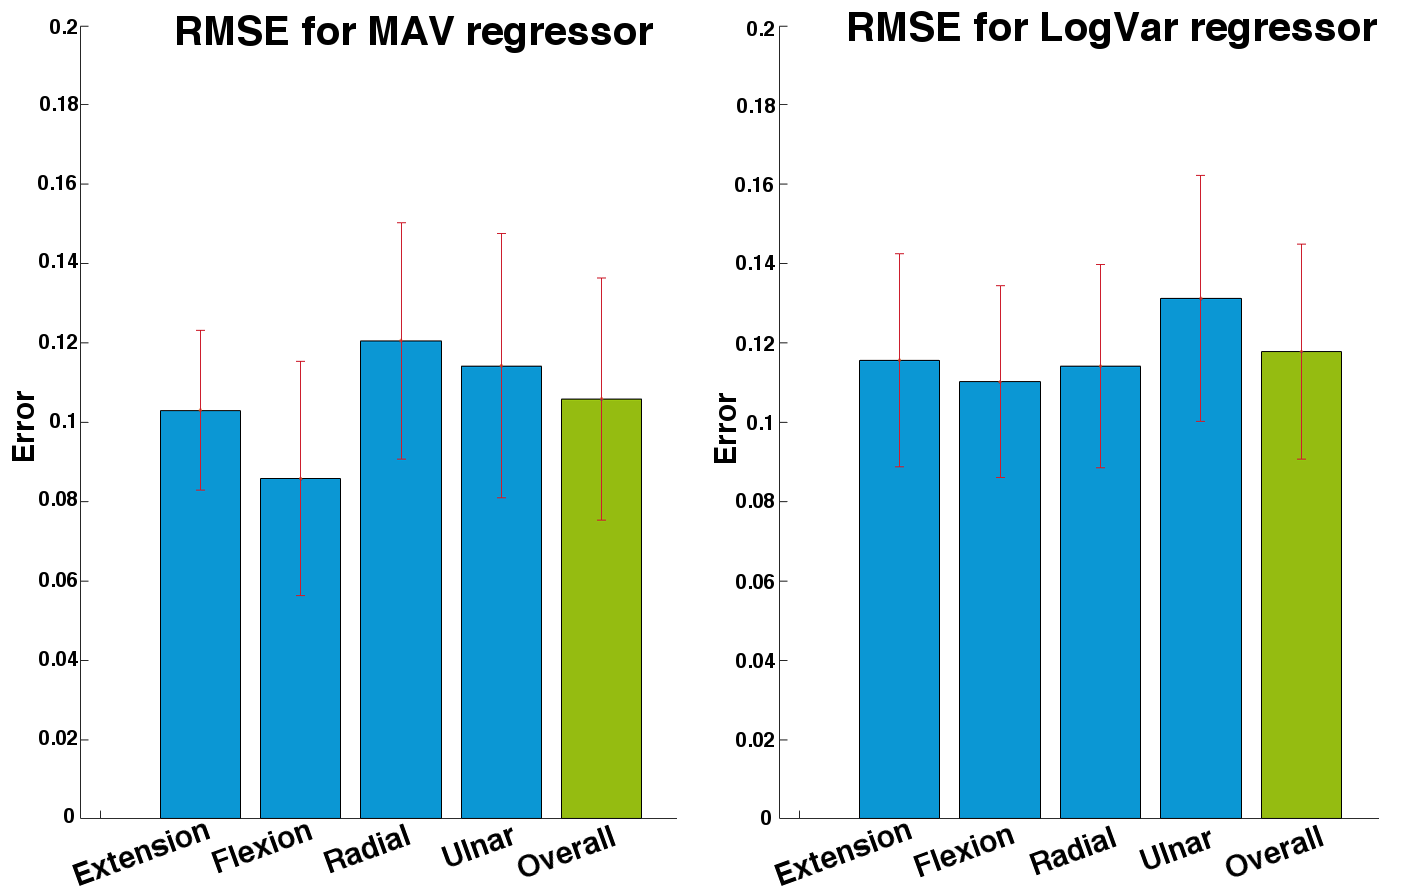
\includegraphics[width=.7\textwidth]{figures/results/gimmeThemRMSEBars}  %<--but is not needed.
	\caption{Bar plot of the error of MAV and the logarithmic variance features for the four hand gestures. The bar chart illustrates the mean error and the error bar illustrates the standard deviation}
	\label{fig:gimmeThemRMSEBars}  %<--give the figure a label, so you can reference!
\end{figure}

The overall mean of the RMSE of MAV is 0.0943 with a standard deviation of $\pm 0.0290$, where the highest mean of a regressor is 0.1088 and the highest standard deviation is $\pm 0.0366$. The overall mean of the RMSE of the logarithmic variance is 0.1107 with a standard deviation of $\pm 0.0298$, where the highest mean of a regressor is 0.1216 and the highest standard deviation is $\pm 0.0402$. MAV then yields a lower mean RMSE and a lower standard deviation than the logarithmic variance - both with the overall RMSE and for the movement with the highest RMSE. 

%%% testing data plot
\subsection{Accuracy of regressors with test data}
This section contains the superimposition of the expected output of the regressors on the output of the regressors fed with test data. The plot in \figref{fig:SuperPoisonLogVarNewData} depicts the superimposition the logarithmic variace trained regressors fed with the test data.

\begin{figure}[H]
	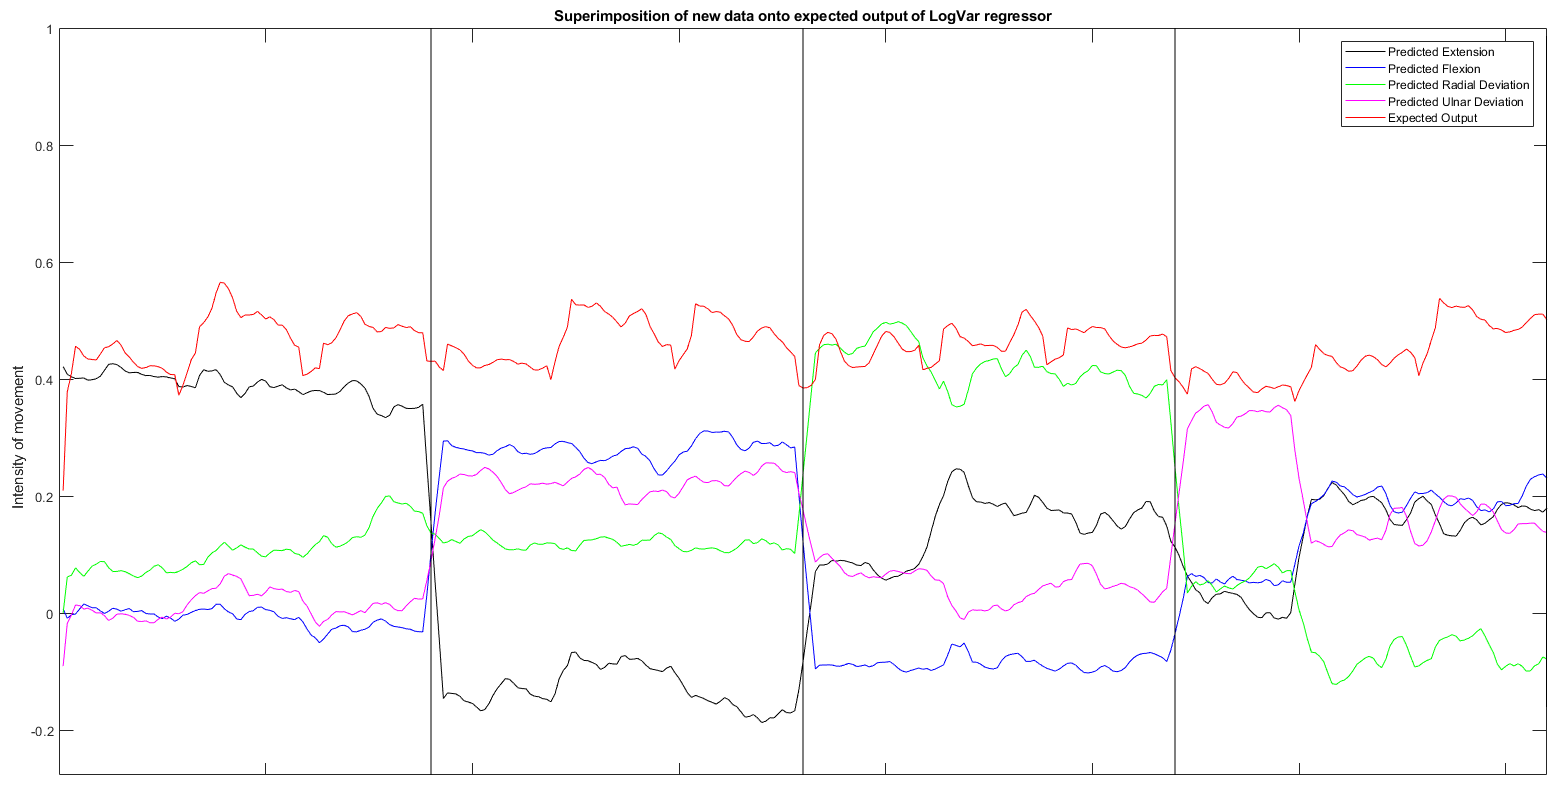
\includegraphics[width=0.7\textwidth]{figures/results/SuperPoisonLogVarNewData}  %<--but is not needed.
	\caption{}
	\label{fig:SuperPoisonLogVarNewData}  %<--give the figure a label, so you can reference!
\end{figure}

It is seen that regressors trained for different movements reacts on the same movement, especially for the flexion and ulnar deviation movement. However, the 

\begin{figure}[H]
	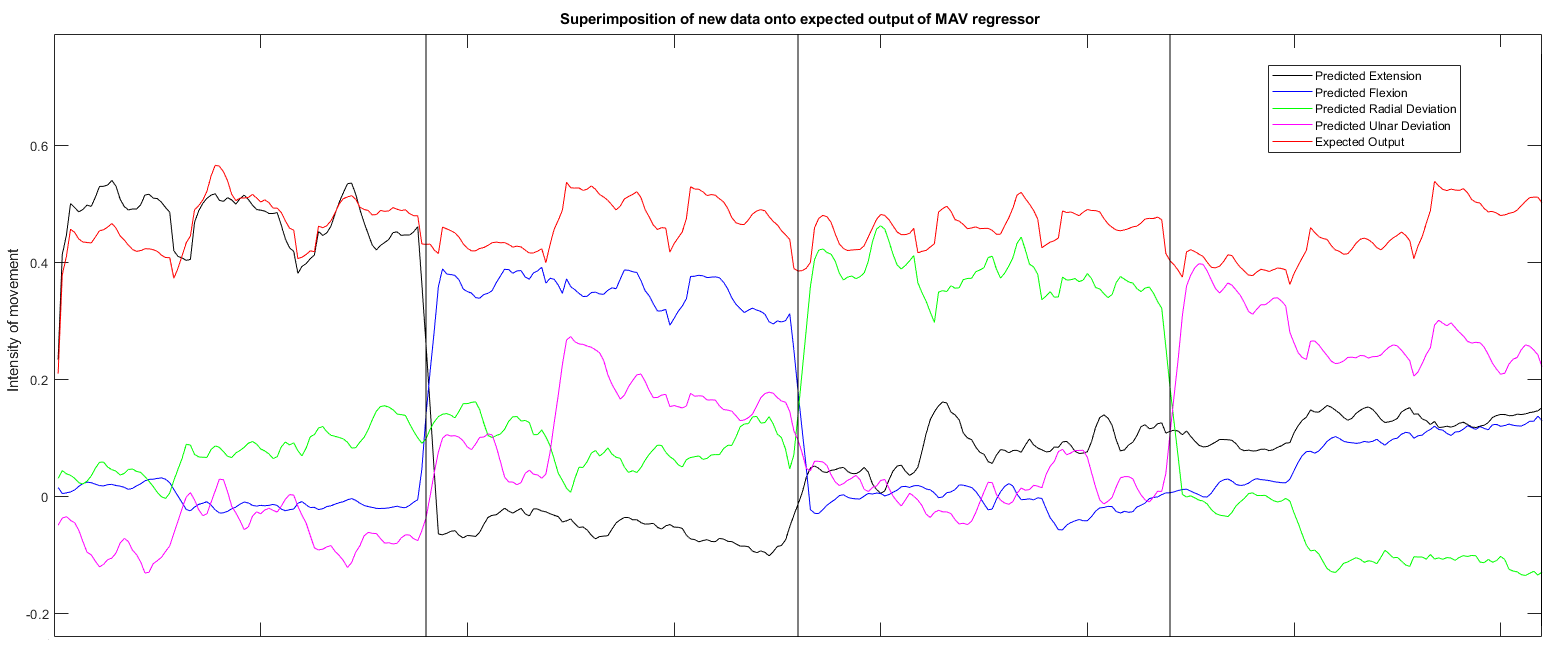
\includegraphics[width=0.7\textwidth]{figures/results/SuperPoisonMavNewData}  %<--but is not needed.
	\caption{}
	\label{fig:SuperPoisonMavNewData}  %<--give the figure a label, so you can reference!
\end{figure}


\begin{figure}[H]
	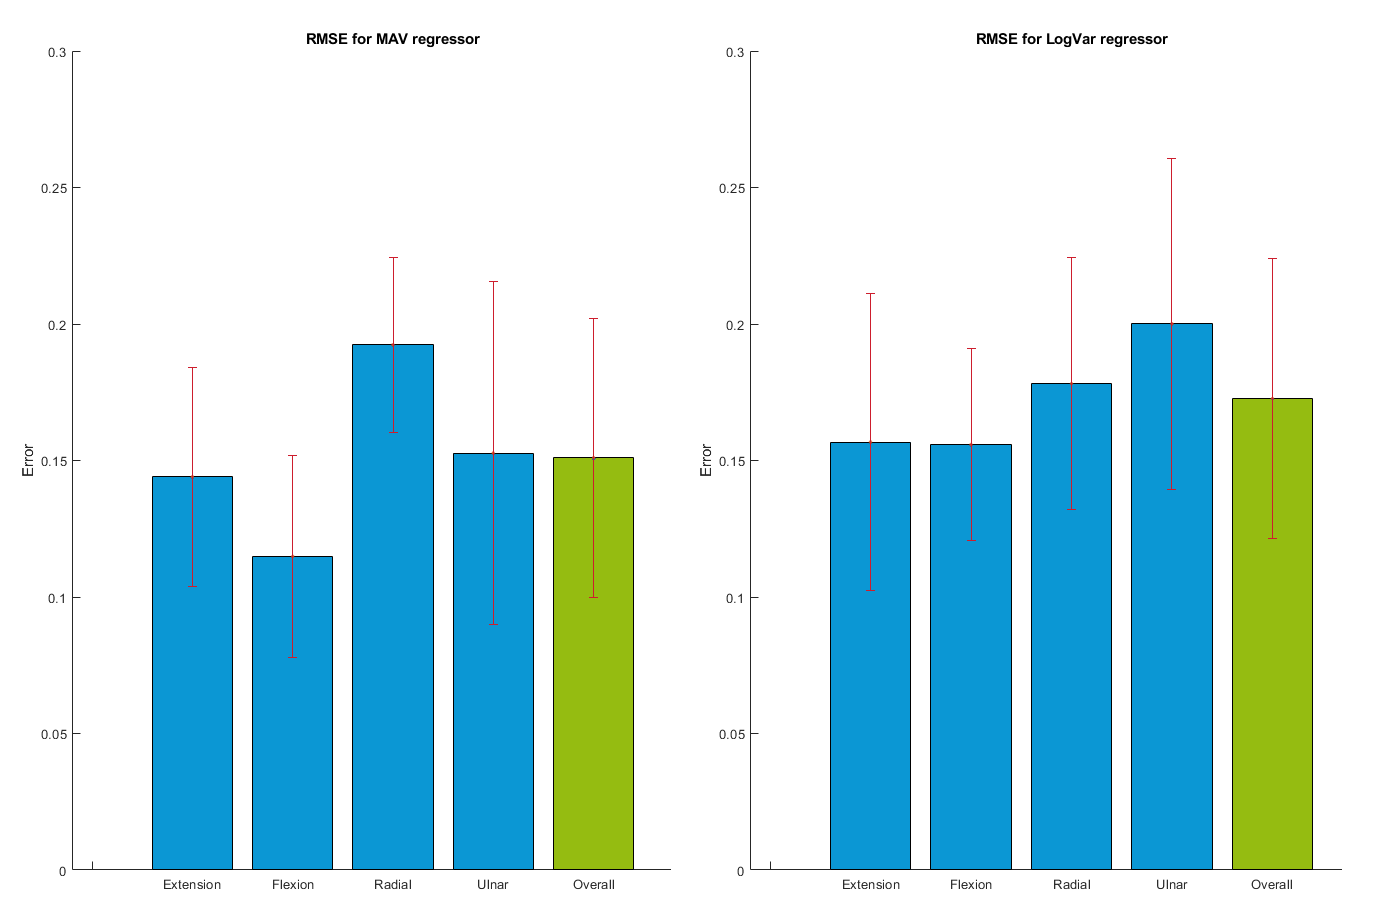
\includegraphics[width=0.7\textwidth]{figures/results/RMSEBarPlotNewData}  %<--but is not needed.
	\caption{}
	\label{fig:RMSEBarPlotNewData}  %<--give the figure a label, so you can reference!
\end{figure}

\begin{figure}[H]
	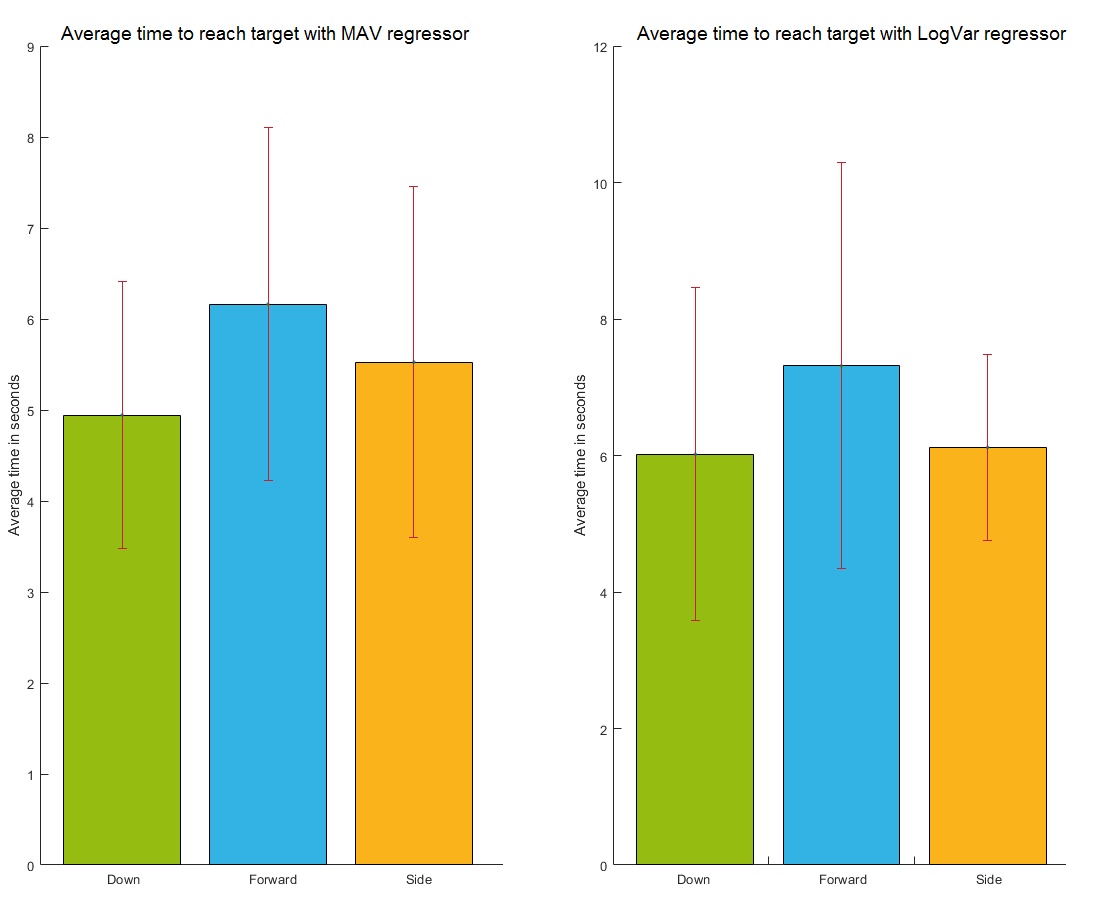
\includegraphics[width=0.7\textwidth]{figures/results/GotItTime}  %<--but is not needed.
	\caption{}
	\label{fig:GotItTime}  %<--give the figure a label, so you can reference!
\end{figure}

\begin{figure}[H]
	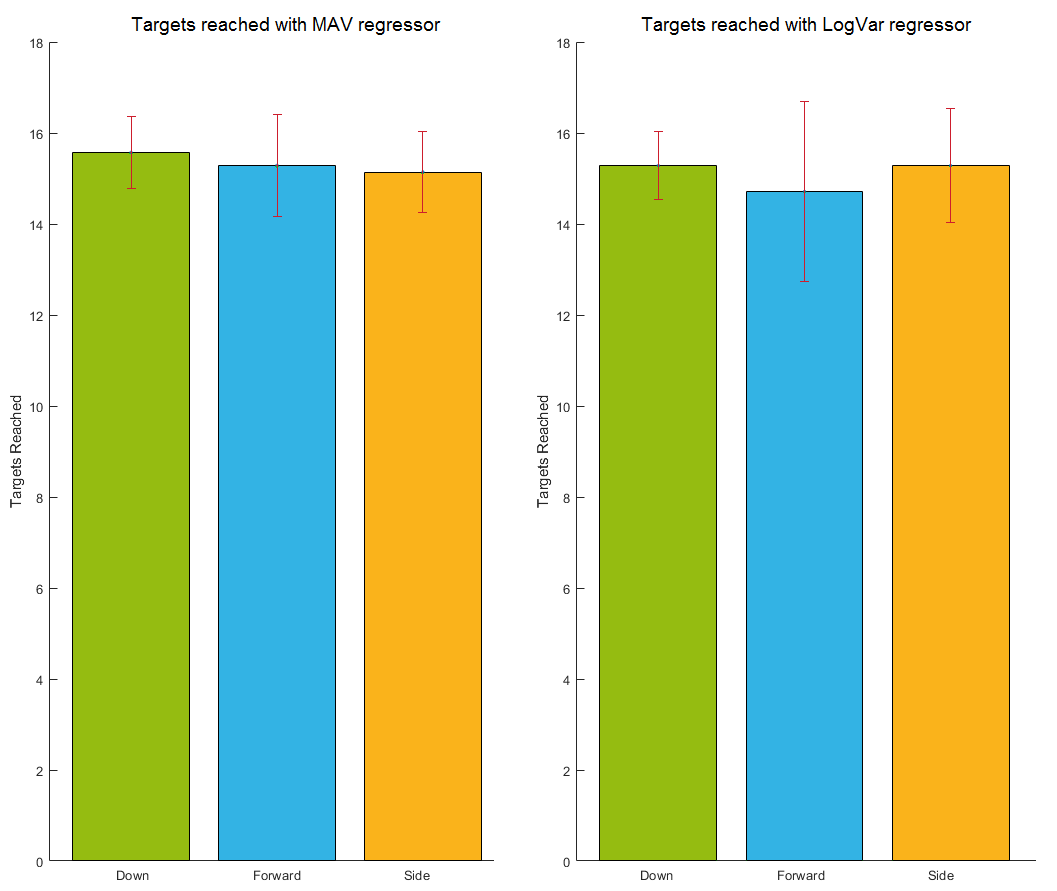
\includegraphics[width=0.7\textwidth]{figures/results/TargetsReached}  %<--but is not needed.
	\caption{}
	\label{fig:TargetsReached}  %<--give the figure a label, so you can reference!
\end{figure}
\section{Performance test}
This section contains the results from the performance test done by the subjects. First of the results from the regressor trained only with EMG data are presented, and afterwards compared to the regressor trained with inclusion of IMU data. The boxplot in \ref{fig:GotItTime} shows the test scores of all limb positions for both features.

\begin{figure}[H]
	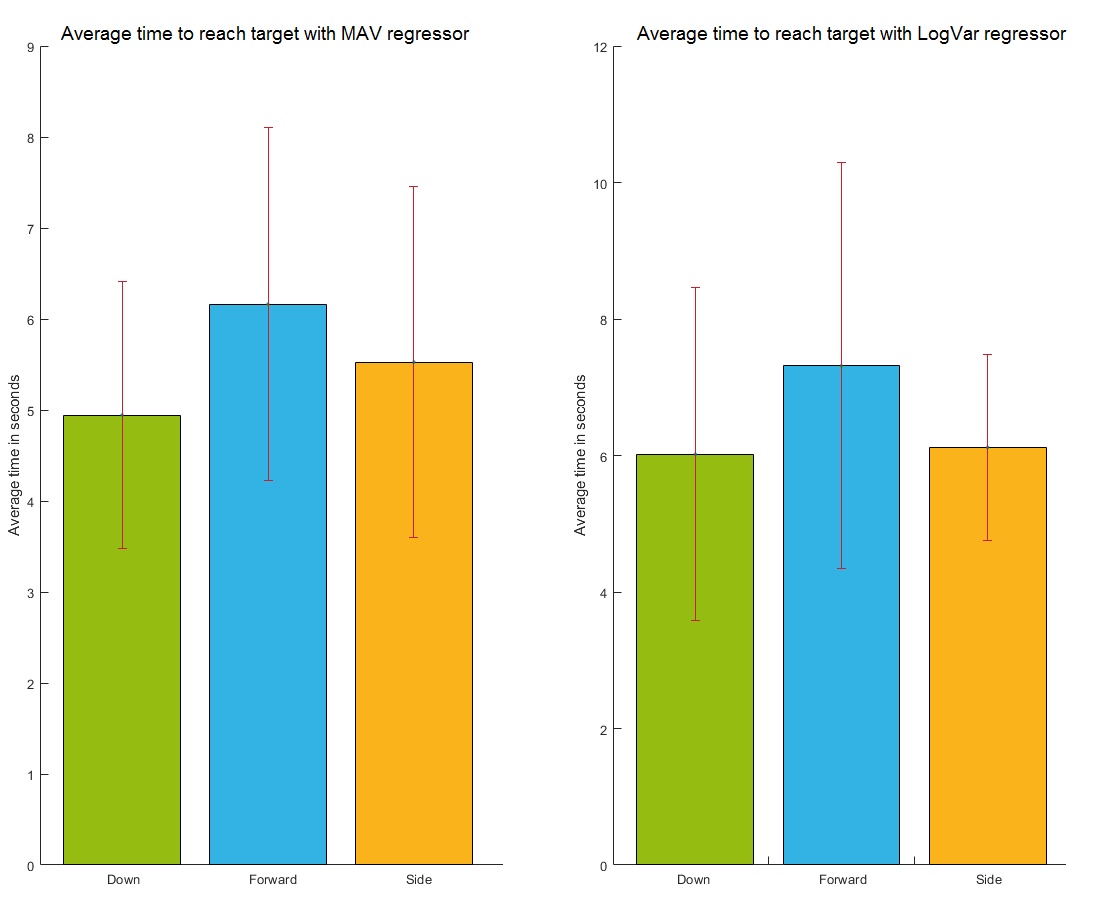
\includegraphics[width=0.7\textwidth]{figures/results/GotItTime}  %<--but is not needed.
	\caption{Calculated performance scores of the regressors. The bar chart illustrates the mean score across all subjects in the different limb positions, and the error bar illustrates the standard deviation}
	\label{fig:GotItTime}  %<--give the figure a label, so you can reference!
\end{figure}

	\begin{center}
		\begin{tabular}{l l l}
			\toprule
			\textbf{Limb position and feature} & \textbf{Overall mean error} & \textbf{Standard deviation}\\
			\midrule
			Down, MAV & 5.3377 & $\pm 1.5696$ \\
			Forward, MAV & 8.1791 & $\pm 4.7145$ \\
			Side, MAV & 6.0490 & $\pm 2.0490$ \\
			Down, LogVar & 6.5404 & $\pm 2.5315$ \\
			Forward, LogVar & 7.9123 & $\pm 3.4572$ \\
			Side, LogVar & 6.9325 & $\pm 2.3036$ \\
			\bottomrule
		\end{tabular}
		\captionof{table}{Test scores for the different limb for MAV and LogVar regressors}
	\end{center}
	
	\begin{center}
		\begin{tabular}{l l}
			\toprule
			\textbf{Feature} & \textbf{P-Value}\\
			\midrule
			MAV & 0.0319 \\
			LogVar & 0.4594 \\
			\bottomrule
		\end{tabular}
		\captionof{table}{P-Values for comparison of the score in different limb positions with MAV and LogVar}
	\end{center}

A one-sample Kolmogorov-Smirnov test was done on the scores from the MAV and LogVar respectively and showed no normality in both score sets(p = $7 * 10^{-20}$, $8 * 10^{-20}$ ). A Friedman's test was therefore applied for statistical analysis. The performance scores between the three limb positions prove not to be significantly different (p = 0.4594), when applying the LogVar trained regressors in the online test. For the MAV trained regressors the performance score between all limb positions can be proven significantly different (p = 0.0319). 

\begin{figure}[H]
	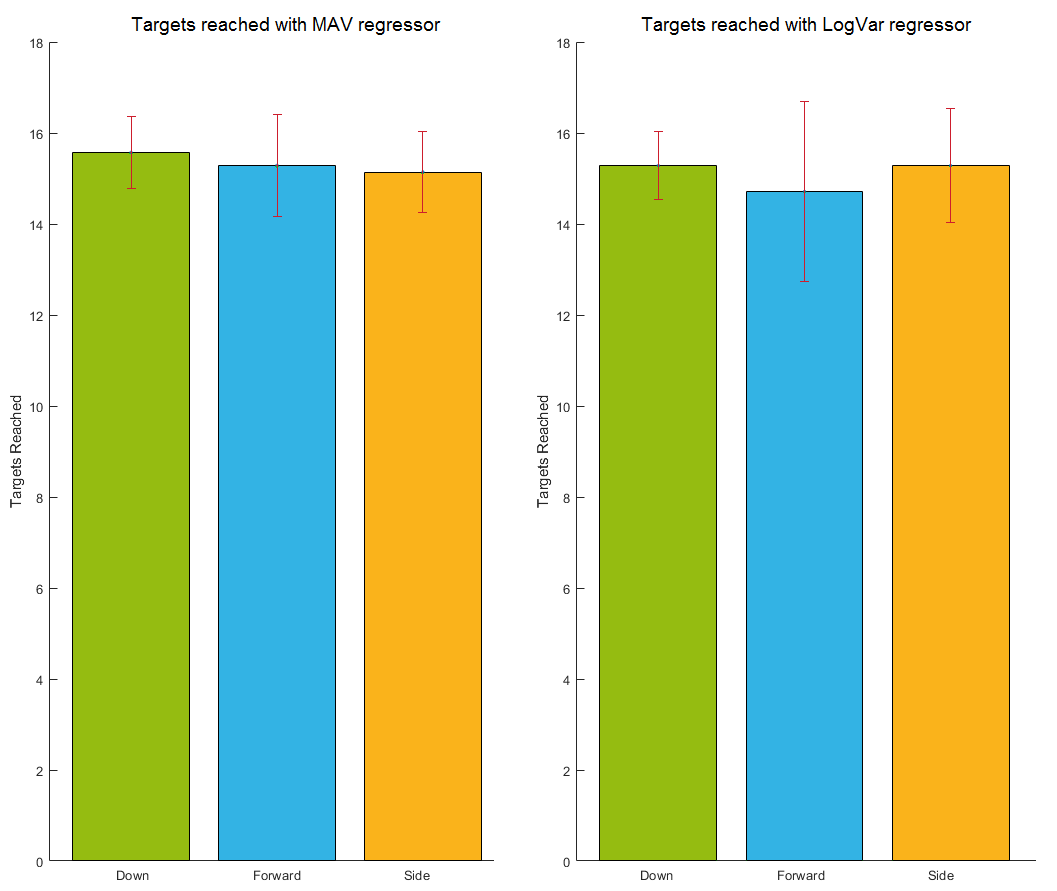
\includegraphics[width=0.7\textwidth]{figures/results/TargetsReached}  %<--but is not needed.
	\caption{The boxplot illustrates the amount of targets reached for the respective limb positions for both features.}
	\label{fig:TargetsReached}  %<--give the figure a label, so you can reference!
\end{figure}

	\begin{center}
		\begin{tabular}{l l l}
			\toprule
			\textbf{Limb position and feature} & \textbf{Overall mean error} & \textbf{Standard deviation}\\
			\midrule
			Down, MAV & 15.5556 & $\pm 0.7265$ \\
			Forward, MAV & 15.1111 & $\pm 1.0541$ \\
			Side, MAV & 15.2222 & $\pm 0.8333$ \\
			Down, LogVar & 15.4444 & $\pm 0.7265$ \\
			Forward, LogVar & 15 & $\pm 1.8020$ \\
			Side, LogVar & 15.3333 & $\pm 1.1180$ \\
			\bottomrule
		\end{tabular}
		\captionof{table}{Targets reached in the target test with the MAV and LogVar regressors.}
	\end{center}

	\begin{center}
		\begin{tabular}{l l}
			\toprule
			\textbf{Feature} & \textbf{P-Value}\\
			\midrule
			MAV & 0.2285 \\
			LogVar & 0.7788 \\
			\bottomrule
		\end{tabular}
		\captionof{table}{P-Values for comparison of the number of reached targets across different limb positions with MAV and LogVar}
	\end{center}
	
The Friedman's statistical test shows no significant difference (p = 0.2285) between the number of targets reached in the different limb positions for the MAV regressor. There was no significant difference (p = 0.7788) between the limb positions for the LogVar regressor either.

%A qualitative examination of the box plot in \ref{fig:TargetsReached} shows no significant difference in targets reached between limb positions and between all limb positions for the two features, which is similar to the Friedman's test results for the time per reached target.

\begin{figure}[H]
	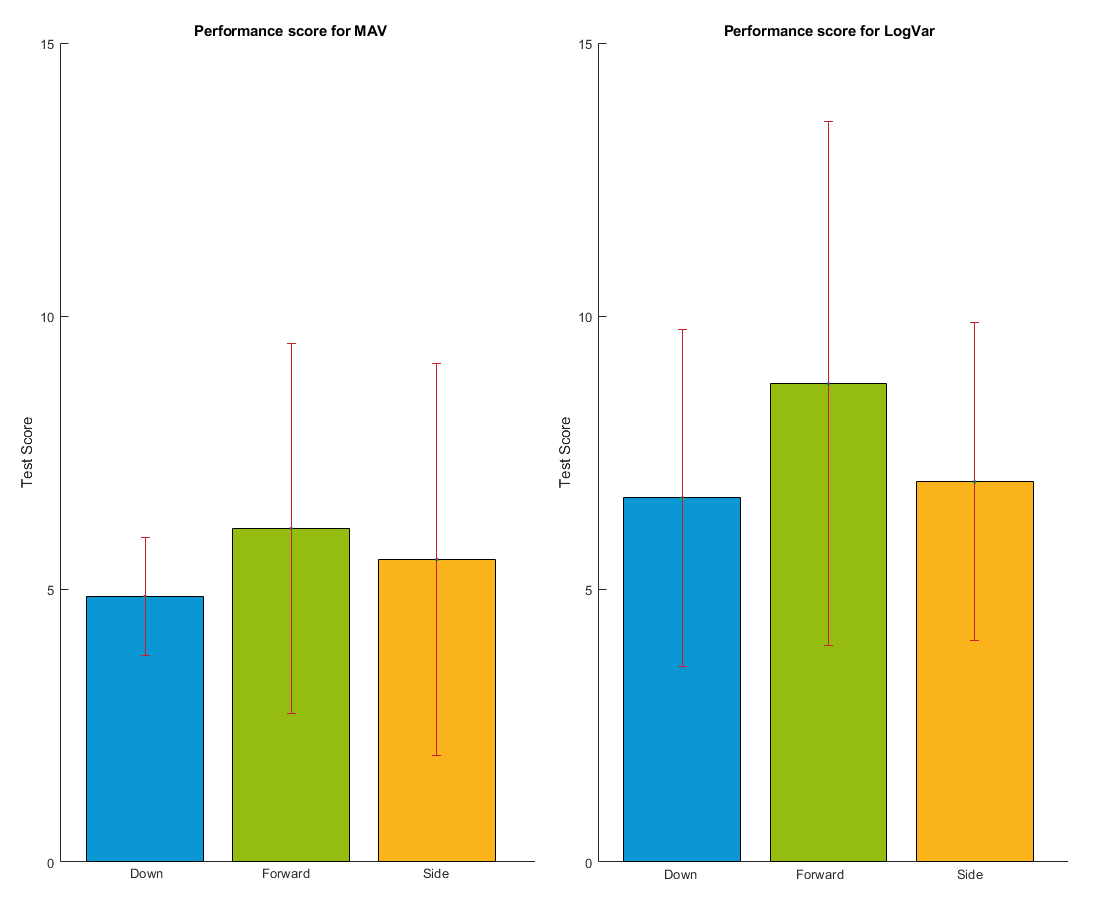
\includegraphics[width=0.7\textwidth]{figures/results/GotItTimeIMU}  %<--but is not needed.
	\caption{Calculated performance scores of the regressors with IMU data included. The bar chart illustrates the mean score across all subjects in the different limb positions, and the error bar illustrates the standard deviation}
	\label{fig:gotItTimeIMU}  %<--give the figure a label, so you can reference!
\end{figure}

	\begin{center}
		\begin{tabular}{l l l}
			\toprule
			\textbf{Limb position and feature} & \textbf{Overall mean error} & \textbf{Standard deviation}\\
			\midrule
			Down, MAV & 4.8661 & $\pm 1.0839$ \\
			Forward, MAV & 6.1094 & $\pm 3.3852$ \\
			Side, MAV & 5.5442 & $\pm 3.5847$ \\
			Down, LogVar & 6.6691 & $\pm 3.0798$ \\
			Forward, LogVar & 8.7595 & $\pm 4.7969$ \\
			Side, LogVar & 6.9652 & $\pm 2.9144$ \\
			\bottomrule
		\end{tabular}
		\captionof{table}{Test scores for the different limb for MAV and LogVar regressors with IMU included.}
	\end{center}
	
		\begin{center}
			\begin{tabular}{l l}
				\toprule
				\textbf{Feature} & \textbf{P-Value}\\
				\midrule
				MAV & 0.8948 \\
				LogVar & 0.2359 \\
				\bottomrule
			\end{tabular}
			\captionof{table}{P-Values for comparison of the score in different limb positions with MAV and LogVar with IMU data included}
		\end{center}

The test with IMU data included shows no significant difference (p = 0.8948) between the test score in different limb positions for the MAV regressor. No difference was proven in the LogVar test (p = 0.2359) either.

\begin{figure}[H]
	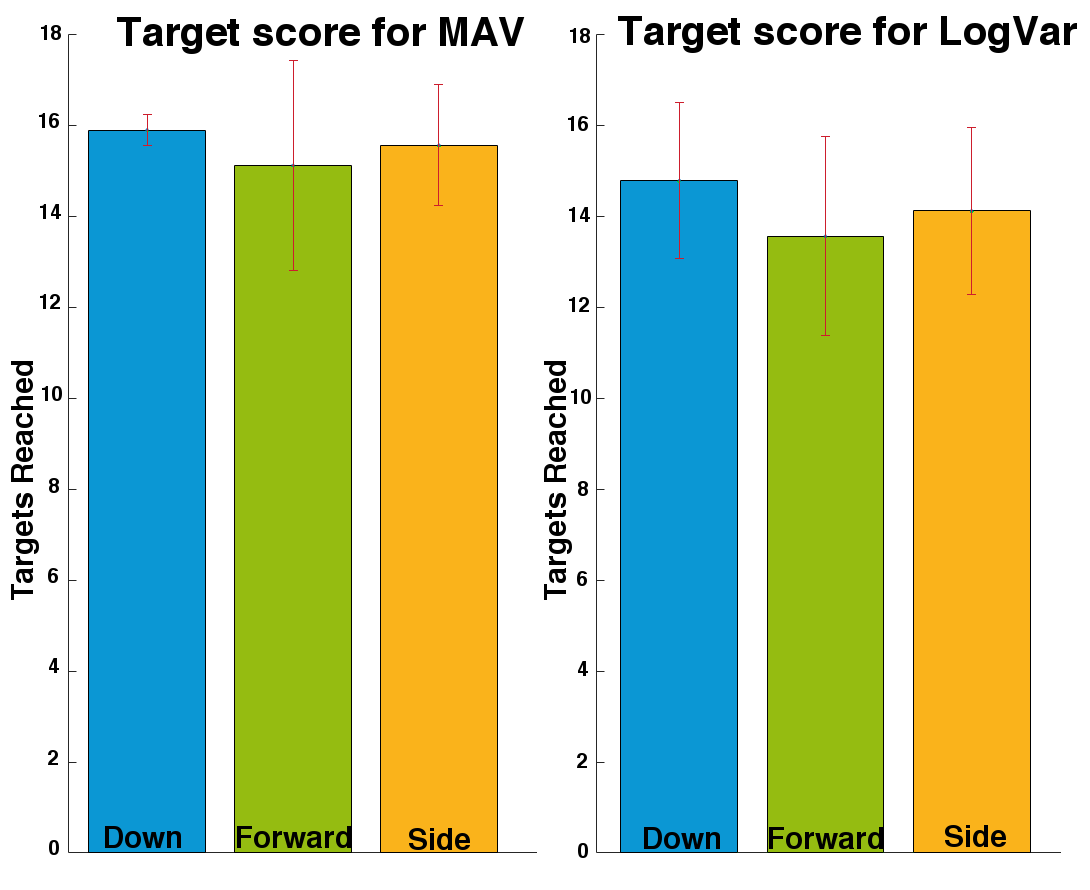
\includegraphics[width=0.7\textwidth]{figures/results/TargetsReachedIMU}  %<--but is not needed.
	\caption{The boxplot illustrates the amount of targets reached for the respective limb positions for both features with IMU data included.}
	\label{fig:TargetsReachedIMU}  %<--give the figure a label, so you can reference!
\end{figure}

	\begin{center}
		\begin{tabular}{l l l}
			\toprule
			\textbf{Limb position and feature} & \textbf{Overall mean error} & \textbf{Standard deviation}\\
			\midrule
			Down, MAV & 15.8889 & $\pm 0.3333$ \\
			Forward, MAV & 15.1111 & $\pm 2.3154$ \\
			Side, MAV & 15.5556 & $\pm 1.3333$ \\
			Down, LogVar & 14.7778 & $\pm 1.7159$ \\
			Forward, LogVar & 13.5556 & $\pm 2.1858$ \\
			Side, LogVar & 14.1111 & $\pm 1.8333$ \\
			\bottomrule
		\end{tabular}
		\captionof{table}{RMSE for the implemented LogVar regressor}
	\end{center}
	
	\begin{center}
		\begin{tabular}{l l}
			\toprule
			\textbf{Compared Features} & \textbf{P-Value}\\
			\midrule
			MAV & 0.4966 \\
			LogVar & 0.0957 \\
			\bottomrule
		\end{tabular}
		\captionof{table}{P-Values for comparison of the number of targets reached in different limb positions with MAV and LogVar with IMU data included}
	\end{center}
	
The number of targets reached in the different limb positions can be proven to be significantly different (p = 0.0957) for the LogVar feature with IMU data included, where the lowest number of targets reached (mean = 13.5556) was found when the subjects pointed their arm forward. There was no significant difference found for the MAV regressor with IMU data included (p = 0.4966).
	
\subsection{Comparison of regressors with and without IMU data}

\begin{figure}[H]
	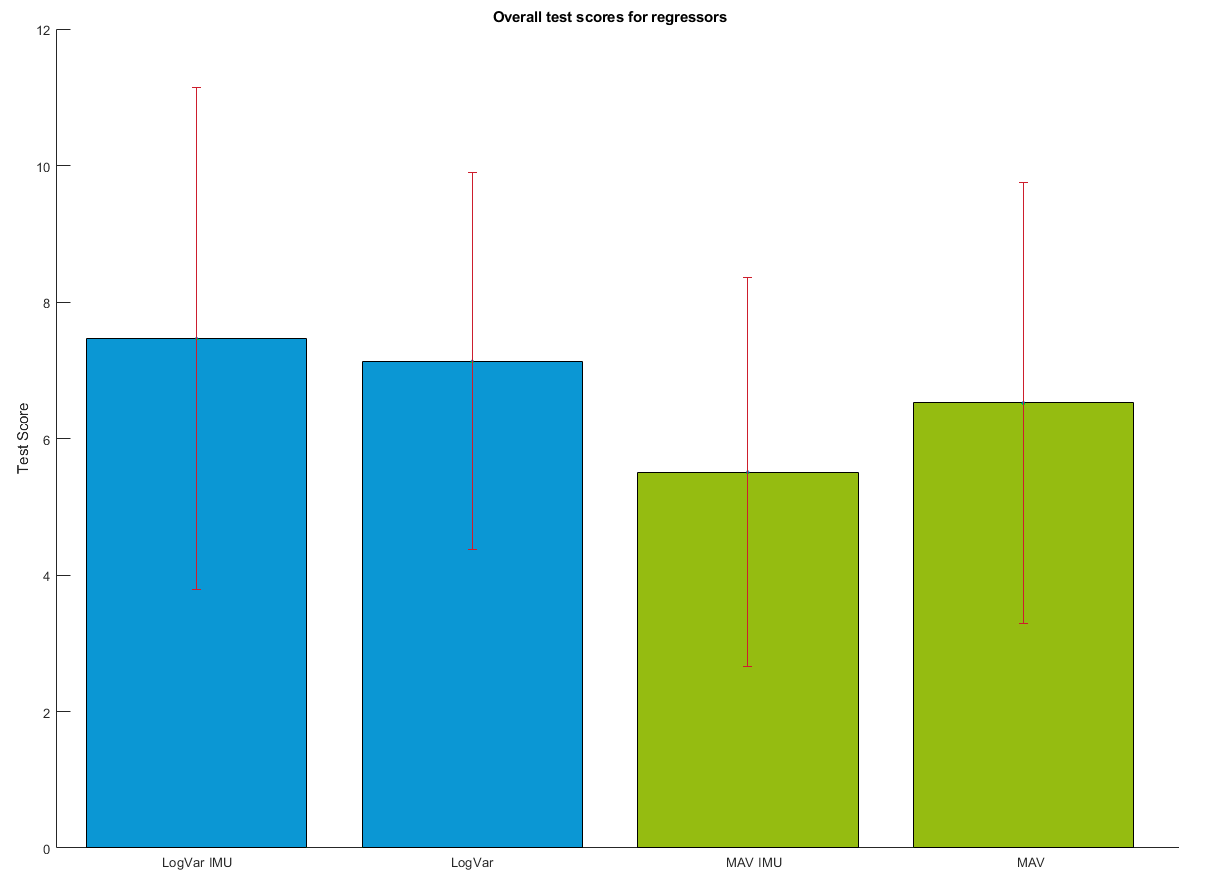
\includegraphics[width=0.7\textwidth]{figures/results/allRegressorBarzTimeScoreForTargetTest}  %<--but is not needed.
	\caption{Calculated overall performance scores of the regressors with and without IMU data included. The bar chart illustrates the mean score across all subjects, and the error bar illustrates the standard deviation}
	\label{fig:gotItTimeOverall}  %<--give the figure a label, so you can reference!
\end{figure}

\begin{center}
	\begin{tabular}{l l l}
		\toprule
		\textbf{Feature} & \textbf{Mean score} & \textbf{Standard deviation}\\
		\midrule
		MAV & 6.5219 & $\pm 3.2253$ \\
		MAV w. IMU & 5.5066 & $\pm 2.8477$ \\
		LogVar & 7.1284 & $\pm 2.7619$ \\
		LogVar w. IMU & 7.4646 & $\pm 3.6740$ \\
		\bottomrule
	\end{tabular}
	\captionof{table}{Average score of the target test for the four regressor designs}
\end{center}

\begin{center}
	\begin{tabular}{l l}
		\toprule
		\textbf{Compared features} & \textbf{P-Value}\\
		\midrule
		LogVar w. IMU, MAV w. IMU & 0.5637 \\
		LogVar, MAV & 0.0833 \\
		LogVar w. IMU, LogVar & 0.5637 \\
		MAV w. IMU, MAV & 0.1779 \\
		\bottomrule
	\end{tabular}
	\captionof{table}{P-Values for comparison of the overall scores of the target tests}
\end{center}

When comparing all performance scores from the two feature trained regression control schemes without IMU, the Friedman's test proves no significant difference (LogVar: 7.1284 s, MAV: 6.5219 s; p = 0.0833). There is no significant difference to be found between LogVar and MAV with IMU data included (LogVar w. IMU: 7.4646, MAV w. IMU: 5.5066, p = 0.5637), and no difference was found between features with and without IMU for either MAV (wo. IMU: 6.5219, w. IMU: 5.5066, p = 0.1779) or LogVar (wo. IMU: 7.1284, w. IMU: 7.4646, p = 0.5637).


\begin{figure}[H]
	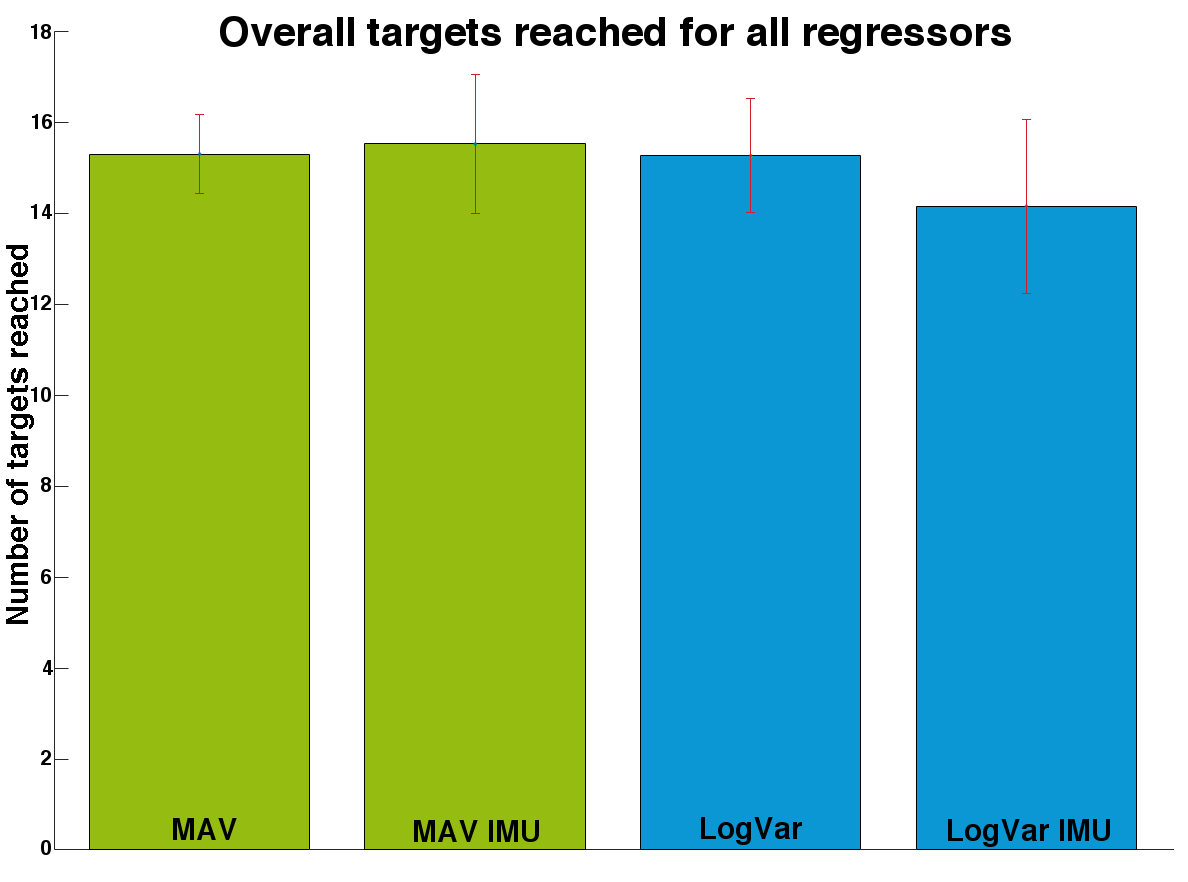
\includegraphics[width=0.7\textwidth]{figures/results/sumMoreBarsWithTargetsReachedForAllRegressors}  %<--but is not needed.
	\caption{The boxplot illustrates the amount of targets reached for all limb positions for the two features with and without IMU data included.}
	\label{fig:TargetsReachedOverall}  %<--give the figure a label, so you can reference!
\end{figure}

\begin{center}
	\begin{tabular}{l l l}
		\toprule
		\textbf{Feature} & \textbf{Overall mean error} & \textbf{Standard deviation}\\
		\midrule
		MAV & 15.2963 & $\pm 0.8689$ \\
		MAV w. IMU & 15.5185 & $\pm 1.5285$ \\
		LogVar & 15.2593 & $\pm 1.2586$ \\
		LogVar w. IMU & 14.1481 & $\pm 1.9156$ \\
		\bottomrule
	\end{tabular}
	\captionof{table}{Average number of targets reached in the target test for the four regressor designs}
\end{center}

		
\begin{center}
	\begin{tabular}{l l}
		\toprule
		\textbf{Compared Features} & \textbf{P-Value}\\
		\midrule
		LogVar w. IMU, MAV w. IMU & 0.0017 \\
		LogVar, MAV & 1 \\
		LogVar w. IMU, LogVar & 0.0016 \\
		MAV w. IMU, MAV & 0.0124 \\
		\bottomrule
	\end{tabular}
	\captionof{table}{P-Values for comparison targets reached in the target tests}
\end{center}

A significant difference was found between LogVar and MAV when IMU was included (LogVar w. IMU: 14.1481, MAV w. IMU: 15.5185, p = 0.0017), and the same was found when including IMU data for both MAV (wo. IMU: 15.2963, w. IMU: 15.5185, p = 0.0124) and LogVar (wo. IMU: 15.2593, w. IMU: 14.1481, p = 0.0016). The performance was similar when comparing the overall number of targets reached for LogVar and MAV (p = 1).

\chapter{Discussion}
\input{contents/yzDiscussion/Discussion.tex}

\chapter{Conclusion}
\section{Conclusion}

This study found that linear regression yields simultaneous and proportional control of multiple degrees of freedom in a stable way independent of limb positions, as it was found that the precision of the regression models enabled the test subjects to perform a target test with similar results independent of the positioning of the arm. Linear regression should be investigated further, as a control scheme with precise, simultaneous and proportional control in more than one limb position. Regression based control schemes could have the potential to be implemented in myoelectric prosthetic devices to improve the functionality, and thereby improving life quality for amputees.


	
\urlstyle{same}
\printbibliography
\cleardoublepage


%% BILAG
%\begin{appendices}
%	
%\end{appendices}


\end{document}
